%\documentclass{cslthse-msc} %% Lund
\documentclass[pregrado]{tesis-usb} %% USB
\usepackage[utf8]{inputenc}
\usepackage{amsmath}
\usepackage{amsfonts}
\usepackage{amssymb}
\usepackage{amsthm}
\usepackage{amsmath}
\usepackage{mathtools}
%%\usepackage{makeidx}
\usepackage{graphicx}

\usepackage{acronym}
\usepackage{amsmath}
\usepackage{amsfonts}
\usepackage{amssymb}



%\usepackage{hyperref}

\usepackage{diagbox}
\usepackage{float}
\usepackage{booktabs}
\usepackage{makecell}


\DeclarePairedDelimiter\abs{\lvert}{\rvert}%
\DeclarePairedDelimiter\norm{\lVert}{\rVert}%

%\geometry{showframe}

% Spanish Changes
%\addto\captionsspanish{% Replace "english" with the language you use
%	\renewcommand{\contentsname}%
%	{Tabla de Contenidos}%
%}

%\author{
%	Christian Alexander Oliveros Labrador \\
%	{\normalsize \href{mailto:christianol_01@hotmail.com}{\texttt{christianol\_01@hotmail.com}}}
%	%\and
%	%Camilla Lekebjer \\
%	%{\normalsize \href{mailto:Camilla.Lekebjer@cs.lth.se}{\texttt{Camilla.Lekebjer@cs.lth.se}}}
%}

%\title{Muestreo Mejorado\\para \\Temporal Anti-Aliasing}
%\subtitle{Un Temporal Anti-Aliasing Mejorado con Sobel}
%%\company{The Corporation AB LTD Inc}
%\supervisors{Ángela Di Serio, \href{mailto:adiserio@ldc.usb.ve }{\texttt{adiserio@ldc.usb.ve}}}{Michael Doggett, \href{mailto:michael.doggett@cs.lth.se}{\texttt{michael.doggett@cs.lth.se}}}
%%\supervisor{John Deer, \href{mailto:jdeer@company.com}{\texttt{jdeer@company.com}}}
%\examiner{Flavius Gruian, \href{mailto:Flavius.Gruian@cs.lth.se}{\texttt{Flavius.Gruian@cs.lth.se}}}

%\date{\today}
%%\date{January 16, 2015}

% estilo de las referencias
\bibliographystyle{plain}

\autor{Oliveros Labrador/Christian Alexander}
\autori{C. A. Oliveros Labrador}
\usbid{13-11000}
\titulo{Muestreo Mejorado para Temporal Anti-Aliasing}
\fecha{Julio~de~2018}\usarcotutor
\agno{2018}
\fechadefensa{\today}
\tutor{Ángela Di Serio}
\usarcotutor
\cotutor{Michael Doggett \mbox{(Lund)}} 
\trabajo{Trabajo de Grado}
\coord{Ingeniería de Computación} %Coloca la coordinación
\grado{Ineniero en Compuatación} %coloca el postgrado
\carrera{Carrera}
\programa{Ingeniería de Computación}
%\juradouno{Ren\'e Escalante}
%\juradodos{Johana Figueroa \mbox{(UC)}}
%\juradotres{Irene Garc\'ia}
%\juradocuatro{José Luis Palacios}

\begin{document}
\selectlanguage{spanish}
\frontmatter
\maketitle
\chapter*{Dedicatoria}

Debe ser elaborada bajo las mismas normas del desarrollo del trabajo y mismo tipo de letra seleccionado (tama\~no 12).

\par Dedicado a la Universidad Sim\'on Bol\'ivar y a su comunidad universidad.

\chapter*{Agradecimientos}

\emph{“El día que dejemos de explorar será el día en que nos comprometemos a vivir en un mundo estancado, desprovisto de curiosidad, vacío de sueños”.}
– Neil deGrasse Tyson

Tengo muchas personas para agradecer por esta increíble aventura. Viniendo de Venezuela, a más de 8000 km de distancia de Suecia, siendo la primera vez que estoy fuera de casa por tanto tiempo, la primera vez que tomo clases sólo en inglés y ser el primer estudiante de intercambio en realizar una Tesis de Maestría en el Departamento de Ciencias de la Computación de la Universidad de Lund, ha sido una experiencia que me cambió la vida.

Me gustaría agradecer a toda mi familia, especialmente a mi papá, Wilmer Oliveros; mi mamá, Raixa Labrador; y mi hermano, Jean Pierre Oliveros, por toda su ayuda y apoyo durante este viaje. Además, me gustaría agradecer a mis amigos de todo el mundo. Gracias por ayudarme a ser lo que soy en este momento y por estar conmigo todo este tiempo.

Me gustaría agradecer a mi supervisor de la Universidad de Lund, el profesor Michael Doggett, por darme esta increíble oportunidad y por ayudarme durante su transcurso. Además, me gustaría agradecer a Pierre Moreau por ayudarme en las veces que estuve estancado.
Además, me gustaría agradecer a mi supervisora de la Universidad Simón Bolívar, la profesora Angela Di Serio; y mi Coordinadora de Ingeniería de la Computación, la profesora Marlene Goncalves, por ayudarme y apoyarme en este increíble viaje.

Finalmente, me gustaría agradecer a la Universidad Lund y la Universidad Simón Bolívar, con un agradecimiento especial a la Oficina Internacional LTH; el Departamento de Ciencias de la Computación de la Universidad de Lund, la Coordinación de Ingeniería de la Computación de la Universidad Simón Bolívar; y la Dirección de Relaciones Internacionales y Cooperación de la Universidad Simón Bolívar, por permitir que los estudiantes aprovechemos estas oportunidades de desarrollo académico y de auto crecimiento.

\begin{figure}[!hbt]
	\centering
	
\includegraphics[scale=0.3]{images/univ_logotypes.png}
\end{figure}

\begin{resumen}
	\textit{Anti-aliasing} es un componente clave de los sistemas modernos de computación gráfica 3D. Para la generación de imágenes en tiempo real en aplicaciones como juegos, es importante aumentar la tasa de muestreo por píxel para mejorar la calidad general de la imagen. Pero aumentar el muestreo puede ser costoso, especialmente para las arquitecturas actuales de \textit{Shading} Diferido. Una solución innovadora a este problema es la técnica de \textit{Temporal Anti-Aliasing} (TAA), que combina muestras de cuadros previos con las muestras del cuadro actual para aumentar efectivamente la tasa de muestreo. En esta tesis, exploraremos métodos para mejorar la calidad del TAA mediante el uso de detección de bordes, tanto de color como de profundidad, y la indexación de triángulos para asegurar que sólo las muestras pertenecientes a los píxeles del cuadro actual se combinen. Nuestro objetivo es reducir el efecto de ghosting y otros artefactos creados con las implementaciones actuales de TAA. La mejora de la calidad se evaluará comparando las imágenes generadas por TAA con las imágenes base (ground truth) generadas mediante el uso de tasas de muestreo mucho más altas, que no serían prácticas en tiempo real. El TAA mejorado se probó utilizando métricas de imágenes, en particular, MSE, PSNR y SSIM, para comparar con la implementación de TAA original y otras técnicas actuales de Anti-Aliasing. Los resultados obtenidos mostraron que las mejoras aplicadas a TAA enriquecieron la calidad de la imagen por encima de las técnicas existentes, con valores de PSNR en torno a 39 y valores de SSIM por encima de 0,99. \\
	\vspace{2cm}\par\noindent {\small{\bf Palabras Clave\/}: TAA, Sobel, Anti-Aliasing, Triangle Indexing, TRAA.}
\end{resumen}

\tableofcontents
\listoffigures
\listoftables

\chapter*{Lista de Acrónimos}
\begin{acronym}
	\acro{USB}[USB]{Universidad Sim\'on Bol\'ivar}
	\acro{DEP}[DEP]{Decanato de Estudios Profesionales}
	\acro{PDF}[PDF]{\textit{Portable Document Format}, Documento en Formato Portable\copyright}
	\acro{PNG}[PNG]{\textit{Portable Network Graphics}, Gráficos de Red Portátiles}
	\acro{2D}[2D]{\textit{Two Dimensions}, Dos Dimensiones}
	\acro{3D}[3D]{\textit{Three Dimensions}, Tres Dimensiones}
	\acro{TAA}[TAA]{\textit{Temporal Anti-Aliasing}}
	\acro{TXAA}[TXAA]{\textit{Temporal X Anti-Aliasing}, donde la X representa alguna versión de TAA}
	\acro{TRAA}[TRAA]{\textit{Temporal Reprojection Anti-Aliasing}, TAA utilizando reproyección (técnica base de TAA)}
	\acro{SSAA}[SSAA]{\textit{Super Sampling Anti-Aliasing}, Anti-Aliasing con Super Muestreo}
	\acro{MSAA}[MSAA]{\textit{Multi Sample Anti-Aliasing}, Anti-Aliasing Multi Muestra}
	\acro{FXAA}[FXAA]{\textit{Fast Approximate Anti-Aliasing}, Anti-Aliasing Aproximado Rápido}
	\acro{SMAA}[SMAA]{\textit{Enhanced Subpixel Morphological Anti-Aliasing}, Anti-Aliasing de Mejora Morfológica de Subpíxeles}
	\acro{AA}[AA]{\textit{Anti-Aliasing}}
	\acro{NOAA}[NOAA]{No \textit{Anti-Aliasing}}
	\acro{API}[API]{\textit{Application Programming Interface}, Interfaz de Programación de Aplicaciones}
	\acro{OpenGL}[OpenGL]{\textit{Open Graphics Library}, Librería Abierta de Gráficos}
	\acro{GPU}[GPU]{\textit{Graphics Processing Unit}, Unidad de Procesamiento de Gráficos}
	\acro{GLSL}[GLSL]{\textit{OpenGL Shading Language}, Lenguaje de Shading de OpenGL}
	\acro{MSE}[MSE]{\textit{Mean Square Error}, Error Cuadrado Medio}
	\acro{RMSD}[RMSD]{\textit{Root Mean Square Deviation}, Desviación de la Raíz Media Cuadrada}
	\acro{RMSE}[RMSE]{\textit{Root Mean Square Error}, Raíz del Error Cuadrado Medio}
	\acro{PSNR}[PSNR]{\textit{Peak Signal-To-Noise Ratio}, Relación Señal a Ruido de Pico}
	\acro{SNR}[SNR]{\textit{Signal-To-Noise Ratio}, Relación Señal a Ruido}
	\acro{SSIM}[SSIM]{\textit{Structural Similarity Index}, Relación Señal a Ruido}

\end{acronym}
\clearpage

\chapter*{Notación Matemática}
\begin{tabular}{ll}
	$\mathbb{R}$ & Conjunto de n\'umeros reales\\
	$M_{m,n}$ & Espacio de las matrices de tama\~no $m$ por $n$ con entradas reales\\
	$\mathcal{L}$ & Operador de Laplace\\
	$\emptyset$ & Conjunto vac\'io
\end{tabular}

\mainmatter

\chapter[Introducción]{Introducción}
La Computación Gráfica moderna se basa en la presentación de escenas hechas de objetos representados como modelos compuestos de polígonos primitivos, siendo el triángulo el más utilizado. Esto para aprovechar su simplicidad y propiedades geométricas para crear algoritmos óptimos que manejen su renderizado (\textit{rendering}). Los triángulos están compuestos por tres vértices, cada uno de los cuales consiste en una posición y otros parámetros asociados, por ejemplo, el color o las normales del triángulo, para la interpolación.

Cuando queremos renderizar los objetos en una escena, tomamos los vértices y los enviamos por el Canal de Renderizado (\textit{Rendering Pipeline}). Allí, son procesados y mapeados a los píxeles de la pantalla con su color respectivo.

Este proceso tiene dos usos principales: Aplicaciones fuera de línea (\textit{offline}), como películas; y aplicaciones en tiempo real (\textit{online}), como los videojuegos. Cada uno de estos usos tiene sus requisitos y limitaciones, pero, para este proyecto, sólo prestaremos atención a las aplicaciones en tiempo real.

El objetivo de este proyecto es mejorar el algoritmo de \textit{Temporal Anti-Aliasing}, técnica que aumenta la calidad de las imágenes, después del proceso de mapeo de triángulos a píxeles, al mezclar cuadros previamente renderizados con los actuales.

El principal requerimiento será lograr la representación de la escena con la mayor calidad posible, con dos restricciones principales: renderizar al menos treinta cuadros por segundo, sin causar una alta pérdida de cuadros por segundo; y trabajar con una cantidad limitada de memoria y ancho de banda, porque necesitamos poder ejecutarlo en una computadora promedio o un dispositivo móvil. \cite{Doggett2017EDAN35, Shreiner2011}


\section{Definición del Problema}
\textit{Temporal Anti-Aliasing} (TAA) es una técnica en tiempo real, relativamente nueva, que proporciona buenos resultados sin incurrir en gran consumo de memoria o costos de procesamiento de otras técnicas. Las técnicas de detección de bordes y de indexación de triángulos, parecen ser buenas candidatas para mejorar la calidad de TAA, al ayudar a reducir los efectos no deseados de \textit{ghosting} y desenfoque  (\textit{blurring}) creados por las implementaciones actuales de TAA.

El objetivo de esta tesis es mejorar la técnica de \textit{Temporal Anti-Aliasing} mediante el uso de detección de bordes, de color y profundidad, y técnicas de indexación de triángulos para reducir el efecto de desenfoque y \textit{ghosting}, sin disminuir la calidad de la imagen renderizada o incurrir en un gran consumo de memoria o alto costo de procesamiento.


\section{Trabajos Relacionados}
La técnica más simple de \textit{Anti-Aliasing} es \textit{Super Sampling Anti-Aliasing} (SSAA, \textit{Anti-Aliasing} con Super Muestreo), que consiste en renderizar a una resolución más alta y luego reducir la imagen a la resolución requerida. Otra técnica es \textit{Multi Sample Anti-Aliasing} (MSAA, \textit{Anti-Aliasing} Multi Muestra), que calcula el color para el píxel final solo una vez \cite{Doggett2017EDAN35}. Podemos conocer de lo que se convertiría en la base del \textit{Temporal Reprojection Anti-Aliasing}  (TAA o TRAA, \textit{Anti-Aliasing} de Reproyección Temporal) en los artículos Aceleración del \textit{Shading} en Tiempo Real con Caching de Reproducción Inversa por Nehab D., Sander PV, Lawrence J., Tatarchuk N., Isidoro JR \cite{Nehab2007}, en el que describen cómo se pueden usar los pixel shaders para guardar información de los píxeles del cuadro anterior y reproyectarla en el siguiente cuadro; y Supermuestreo Amortizado por Yang L., Nehab D., Sander PV, Sitthiamorn P., Lawrence J., Hoppe H. \cite{Yang2009} en el que describen cómo utilizar la reproyección de cuadros previos  en el actual, como método de \textit{Anti-Aliasing} en tiempo real.

A continuación, encontramos técnicas de Post-Procesamiento como \textit{Fast Approximate Anti-Aliasing} (FXAA, \textit{Anti-Aliasing} Aproximado Rápido) por Timothy Lottes \cite{Lottes2009} que usa una forma de detección de bordes para corregir el \textit{aliasing} mientras es compatible con la Arquitectura de \textit{Shading} Diferido (\textit{Deferred Shading Architecture}). También tenemos la implementación de Crytek del \textit{Temporal Anti-Aliasing} (TAA o TXAA) explicada por Tiago Sousa en su presentación Métodos de \textit{Anti-Aliasing} en CryENGINE 3 \cite{JIMENEZ2011_SIGGRAPH11}.

También disponemos de la técnica \textit{Enhanced Subpixel Morphological Anti-Aliasing} (SMAA, \textit{Anti-Aliasing} de Mejora Morfológica de Subpíxeles) de Jorge Jiménez, José I. Echeverría, Tiago Sousa y Diego Gutiérrez \cite{Jimenez2012} que utiliza una técnica de reconstrucción de bordes más compleja, al mismo tiempo que puede trabajar con SSAA, MSAA y una forma básica de TAA.

Finalmente, tenemos las implementaciones TRAA de Ke Xu para Uncharted 4 y Lasse Fuglsang para Inside, que implementan nuevos avances como el \textit{Color Clipping Box} (Caja de Recorte de Colores) y el Filtro de Nitidez (\textit{Sharpen Filter}). Estas dos últimas implementaciones se utilizan como base de esta tesis. \cite{Fuglsand2016, XU2016}


\section{Contribución}
Esta tesis mejora los últimos avances de Ke Xu y Lasse Fuglsang \cite{Fuglsand2016, XU2016}. Proponemos el uso del Operador de Sobel para realizar detecciones de bordes y técnicas de indexación de triángulos para detectar píxeles que se consideran con aliasing. Una vez tenemos estos píxeles detectados, usamos su información para cambiar la forma en la que se rechazan los colores de los cuadros anteriores, a fin de reducir los artefactos de \textit{ghosting} (\textit{ghosting artifacts})  y desenfoque que tiene \textit{Temporal Anti-Aliasing}.

\chapter{Marco Tecnológico}
En este capítulo, explicaremos qué herramientas se utilizaron en esta tesis y por qué.

\section{C++ y el Bonobo Framework}
Utilizamos C ++ y el \textit{Bonobo Framework} para implementar todas las mejoras realizadas en esta Tesis. C ++ es un lenguaje de programación de propósito general, compilado, con funciones imperativas, programación orientada a objetos y administración de memoria de bajo nivel. Lo usamos por su rendimiento, especialmente para aplicaciones de computación gráfica en tiempo real, y por su amplia base de conocimiento.

El \textit{Bonobo Framework} es la base de los cursos de laboratorio de Computación Gráfica (EDAF80) y Computación Gráfica de Alto Rendimiento (EDAN35) de la Universidad de Lund. Fue desarrollado en C ++ y proporciona un motor de renderizado que encontramos fácil de modificar y usar, especialmente, como la base en la que desarrollamos nuestras mejoras.


\section{OpenGL y GLSL}
Usamos esta \textit{Application Programming Interface} (API, Interfaz de Programación de Aplicaciones) porque es la base del sistema de renderización del Bonobo Framework, el cual modificamos para desarrollar nuestras mejoras, y por su compatibilidad multiplataforma. La \textit{Open Graphics Library} (OpenGL, Librería Abierta de Gráficos) es una API de computación gráfica de código abierto, multiplataforma, que maneja 2D y 3D, y permite abstraer al programador de interactuar directamente con la Unidad de Procesamiento de Gráficos (GPU) para lograr una renderización acelerada por hardware. Además, proporciona al programador un Canal de Renderizado de Gráficos (\textit{Rendering Pipeline}), que normalmente se implementa directamente en hardware.

Usamos el \textit{OpenGL Shading Language} (GLSL, Lenguaje de \textit{Shading} de OpenGL) para implementar TAA y nuestras mejoras, como es parte del estándar de OpenGL. GLSL es un lenguaje para \textit{shading} de alto nivel, que permite a los programadores un mayor control del Canal de Renderizado de Gráficos, sin requerir el uso del lenguaje ensamblador de OpenGL o lenguajes específicos de cada hardware.


\section{MATLAB}
Elegimos MATLAB como el entorno donde desarrollamos nuestro marco de pruebas debido a la alta calidad de sus herramientas, su amplia base de conocimientos y sus capacidades de creación rápida de prototipos.

MATLAB es un entorno de cómputo numérico multi-paradigma propietario. Comúnmente utilizado para ciencia, ingeniería y economía. Es popular para aplicaciones de procesamiento de imágenes debido a su amplia biblioteca de algoritmos para este propósito, incluidas las métricas de imágenes.



\chapter{Marco Teórico}
En este capítulo, explicaremos toda la información teórica que es la base de esta tesis, desde la teoría de base de Computación Gráfica hasta las Métricas de Imágenes utilizadas.

\section{Canal de Renderizado}
El Canal de Renderizado Gráfico actual se puede simplificar en tres etapas: \textit{Vertex Shader}, que procesa la geometría asociada con los vértices y los prepara para el siguiente paso; \textit{Rasterizer}, que mapea los triángulos a píxeles en la pantalla, calcula su visibilidad e interpola los parámetros de los vértices para cada píxel cubierto por el triángulo; y el \textit{Pixel Shader} (o \textit{Fragment Shader}) que toma los píxeles visibles del \textit{Rasterizer} y los colorea. La Figura \ref{fig:graphpipeline} es un ejemplo del Canal de Renderizado simplificado.

\begin{figure}[!hbt]
	\centering
	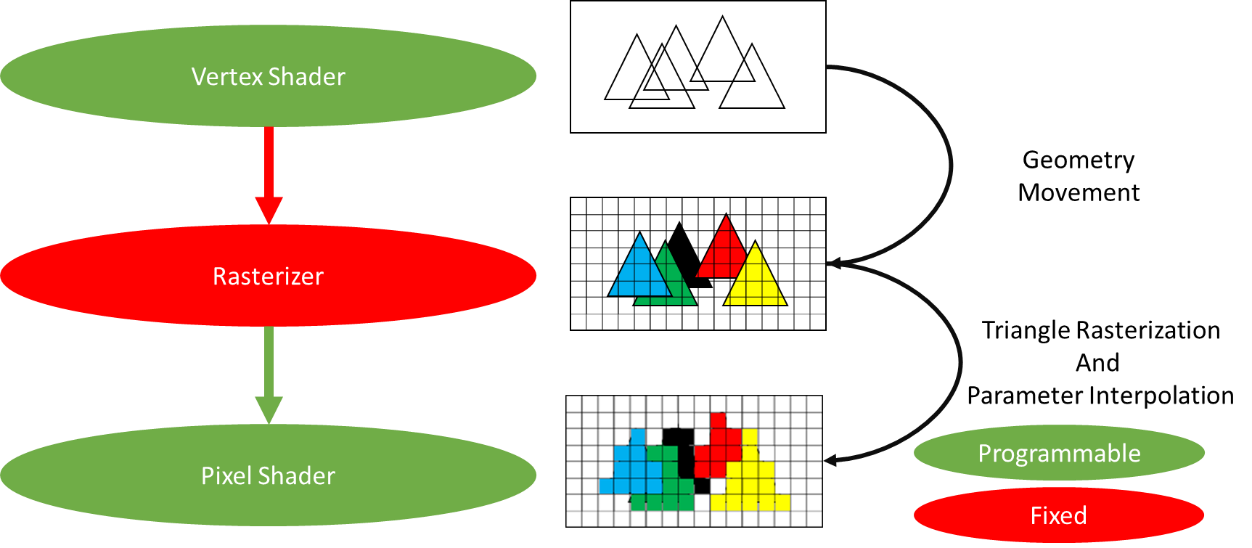
\includegraphics[scale=0.7]{images/graphics_pipeline.png} 
	\caption{Canal de Renderizado, basado en la 5ta clase de EDAF80.~\cite{Doggett2017EDAF80}}\label{fig:graphpipeline}
\end{figure}

Es importante tener en cuenta que las etapas de \textit{Vertex} y \textit{Pixel Shaders} son controlables por el programador usando programas especiales llamados \textit{Shaders}; estos proporcionan una forma para controlar el hardware de renderizado. Por el contrario, el Rasterizer no está controlado por el programador y se maneja por completo mediante una función fija de hardware. \cite{Doggett2017EDAF80}

Este proceso de rasterización es importante para nosotros porque de allí donde provienen algunos de los errores corregidos por \textit{Temporal Anti-Aliasing}.


\section{Proceso de Rasterización}
Durante el proceso de rasterización, a cada triángulo se le realiza una prueba para establecer qué píxeles está cubriendo. Mientras se hace, cada píxel se está probando para descubrir si está cubierto por otro triángulo.

En la Figura \ref{fig:rasterizationproc} tenemos un ejemplo del Proceso de Rasterización. En la imagen de la izquierda, tenemos los triángulos como superficies continuas antes de enviarlos al Rasterizer y, en la imagen de la derecha, tenemos triángulos mapeados a los píxeles en la pantalla después de pasar por el \textit{Rasterizer}.

\begin{figure}[!hbt]
	\centering
	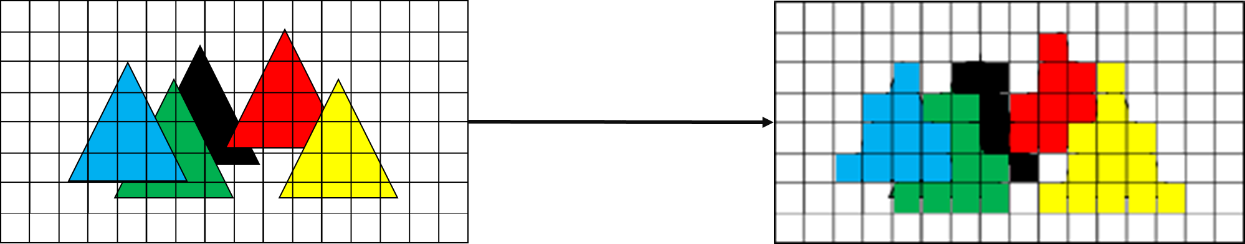
\includegraphics[scale=0.75]{images/rasterization_process.png} 
	\caption{Ejemplo de los resultados del Proceso de Rasterización.
		\emph{Nota}: se agregaron colores para diferenciar los triángulos, pero solo se agregarían en la etapa del \textit{Pixel Shader}.
	}\label{fig:rasterizationproc}
\end{figure}

Debido a que estamos mapeando un triángulo continuo a un número finito de píxeles, enfrentamos el problema de los píxeles parcialmente cubiertos y cómo determinar cuánto es suficiente para calificarlos como cubiertos, la Figura \ref{fig:partialcover} muestra ejemplos de este problema. Esto se resuelve calculando si el centro del píxel está cubierto por la geometría del triángulo. Este proceso es susceptible a errores debido a la precisión de la representación utilizada para los vértices.

\begin{figure}[!hbt]
	\centering
	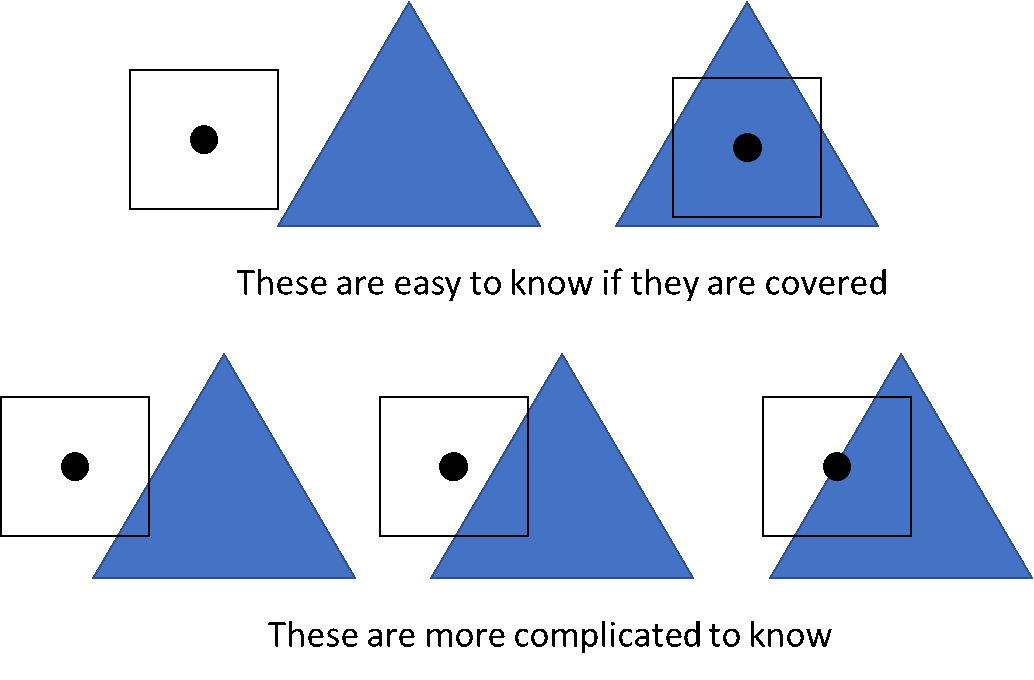
\includegraphics[scale=0.5]{images/edge_testing.png} 
	\caption{Ejemplo del problema de Cobertura Parcial, basado en la segunda clase de EDAN35. ~\cite{Doggett2017EDAN35}}\label{fig:partialcover}
\end{figure}

Este proceso nos muestra que lo que se renderiza en la pantalla, es una aproximación a lo que se representa en la escena, ya que los píxeles solo pueden ser cubiertos con un triángulo a la vez. \cite{Moller2007, Doggett2017EDAN35}


\section{El Problema del Aliasing}
Cuando mapeamos una representación continua en una finita, vamos a generar errores. Como explican Edward Angel y Dave Shreiner en su libro (página 413) \cite{Shreiner2011}, podemos interpretar el proceso de renderización como el muestreo de una función continua $f(x, y)$, que representa el color de la escena en ese punto, a una cuadrícula de píxeles $n\times m$ en la que suponemos que el punto $f_{ij}$ es el valor de $f$ sobre un área pequeña; reconstruyendo la función $f$, para mostrar la imagen en la pantalla, usando solo lo que sabemos de las muestras finitas. La herramienta matemática utilizada para evaluar los problemas de este proceso es el Análisis de Fourier, que establece que una función se puede descomponer en un conjunto de sinusoides, posiblemente en un número infinito de frecuencias. Para el análisis de imágenes bidimensionales, podemos pensar en la función $f$ como un conjunto de sinusoides en dos frecuencias espaciales.

Para esta tesis, usaremos la primera parte del Teorema de Muestreo de Nyquist, como una herramienta para ilustrar por qué aparecen problemas de aliasing y se relacionan con problemas de muestreo. \\

\emph{'' Teorema de Muestreo de Nyquist (Parte 1): Las muestras ideales de una función continua contienen toda la información de la función original si y solo si la función continua se muestrea a una frecuencia mayor que el doble de la frecuencia más alta en la función. }

\emph{La Frecuencia de Nyquist se define como la mitad de la frecuencia de muestreo, que es la frecuencia más baja que no puede estar en los datos para evitar el \textit{aliasing} ''.
} 


Tomado de la página 415 del libro de Edward Angel y Dave Shreiner. \cite{Shreiner2011} \\

Como explican Edward Angel y Dave Shreiner, este muestreo idealizado supone que podemos tomar un número infinito de muestras por frecuencia de muestreo, que no podemos hacer en la práctica. El Problema de \textit{Aliasing} que se experimenta en la Computación Gráfica, proviene de no poder tomar muestras según lo requerido por el Teorema de Muestreo de Nyquist, creando bordes desiguales que aparecen en el proceso de rasterización (\textit{Aliasing} Espacial) y saltos entre objetos en movimiento (\textit{Aliasing} Temporal), de acuerdo con Doggett y Wronski ~\cite{Doggett2017EDAN35, Wronski2014}. La Figura \ref{fig:aliasingexample} muestra un ejemplo de Aliasing Espacial. Se han propuesto y utilizado muchas soluciones para resolver el problema de \textit{Aliasing}, como por ejemplo la familia de soluciones \textit{Super Sampling Anti-Aliasing} (SSAA), que trabaja con frecuencias más altas que las requeridas a costa de mayores requerimientos de espacio.

\begin{figure}[!hbt]
	\centering
	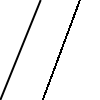
\includegraphics[scale=0.6]{images/aliasing_example.png} 
	\caption{Imagen Base de una línea frente a su Aproximación con \textit{Aliasing}.}\label{fig:aliasingexample}
\end{figure}

\section[Mapeado de Sombras y la Arquitectura de Shading Diferido]{Mapeado de Sombras y \\ la Arquitectura de Shading Diferido}

Como humanos, esperamos que los objetos reaccionen de cierta forma a las luces de una escena, tomando en cuenta la geometría de los objetos, porque las luces y sombras contribuyen con la información espacial a una imagen. En especial, las sombras nos dan una sensación de tamaño y distancia.

Según lo explicado por Doggett \cite{Doggett2017EDAN35}, bajo de la Canal de Renderizado Gráfico basado en el Rasterizer , el proceso de cálculo de la sombra es difícil de realizar. El \textit{Rasterizer} no sabe si los objetos están cubiertos o no por una fuente de luz, por lo que debemos encontrar un método para calcular si un objeto está en la sombra. Este proceso se denomina Mapeado de Sombras, consiste en representar la escena a través de la perspectiva de cada  fuente de luz y luego realizar pruebas en la perspectiva de la cámara, para establecer si el objeto se ve afectado por la luz o si está en sombras.

Pero, como es de esperar, renderizar la escena varias veces es costoso y necesitamos una forma de reducir el costo tanto como podamos. La Arquitectura de \textit{Shading} Diferido proporciona esa solución para realizar el \textit{Shading}, utilizando una operación que podría ser costosa, a solo píxeles visibles y así evitar desperdiciar recursos realizando el \textit{Shading} a píxeles de geometrías que están cubiertas por otros objetos. Esta arquitectura funciona renderizando primero la escena, sin cálculos de \textit{Shading}, en un buffer llamado Buffer de Geometría (\textit{Geometry Buffer}). Allí, se guarda información sobre colores, normales, profundidades, información específica del objeto para interactuar con luces, etc. para uso futuro. 

Después de llenar el Buffer de Geometría, llevamos a cabo la técnica de Mapeado de Sombras, que aprovecha la Arquitectura de \textit{Shading} Diferido para calcular la forma en que las luces afectan sólo a los píxeles visibles; calculamos el Mapa de Sombreado de cada fuente de luz realizando cálculos de profundidad únicamente. Posteriormente, calculamos y guardamos el efecto de cada luz usando los Mapas de  Sombreado.

Al final, tomamos la información de las luces, sombras y el Buffer de Geometría para renderizar la escena con iluminación.


\section{Anti-Aliasing}
Como hemos explicado, hay dos tipos principales de \textit{Aliasing}, Espacial y Temporal. Las soluciones \textit{Anti-Aliasing} proporcionan mejoras contra los artefactos creados por cualquiera de esos tipos a costa de un mayor tiempo de renderizado. Para aplicaciones en tiempo real, este aumento del tiempo de renderización limita qué soluciones Anti-Aliasing son factibles de aplicar.

Otro factor importante para decidir qué técnica \textit{Anti-Aliasing} utilizar,  es cómo se comporta con las arquitecturas actuales. Por ejemplo, las primeras  soluciones Anti-Aliasing no funcionan con el \textit{Shading} Diferido.


\subsection{Super Sampling Anti-Aliasing (SSAA)}
Esta técnica consiste en renderizar la escena a $4$ veces el tamaño de la pantalla y luego promediar el área $4\times 4$ alrededor de cada pixel para calcular el resultado \cite{Doggett2017EDAN35}. Proporciona buenos resultados, pero requiere más tiempo de renderizado y un gran uso de memoria.

\subsection{Multi Sample Anti-Aliasing (MSAA)}
MSAA consiste en tomar varias muestras por píxel; en cada muestra, se calculan los valores de profundidad, pero solo se computa un color para el triángulo rasterizado. Esta solución proporciona buenos resultados a costa de un mayor uso de memoria para cálculos de profundidad.

El mayor problema que tiene esta técnica es que no funciona correctamente con el \textit{Shading} Diferido \cite{Doggett2017EDAN35}. Esto hace que sea complicado de utilizar con los Canales de Renderización actuales, que normalmente requieren otras correcciones para reducir los artefactos creados cuando se aplica con \textit{Shading} Diferido.


\subsection{Fast Approximate Anti-Aliasing (FXAA)}
FXAA es una técnica de \textit{Anti-Aliasing} que se utiliza durante el posprocesamiento. Esta funciona al detectar bordes en las imágenes renderizadas, para luego suavizarlos. \cite{Lottes2009}

Es relativamente barata en comparación con MSAA y proporciona resultados relativamente buenos, sus capacidades de suavizado están limitadas por la cantidad de información que la detección de bordes puede obtener en una sola pasada y proporciona resultados relativamente buenos para el \textit{Aliasing} Temporal.

\subsection{Enhanced Subpixel Morphological Antialiasing (SMAA)}
SMAA es una técnica de post-procesamiento basada en \textit{Morphological Anti-Aliasing} (Anti-Aliasing Morfológico). Funciona mediante la reconstrucción de bordes y sus alrededores para regenerar la información de subpíxel perdida por aliasing. \cite{Jimenez2012}

\section{Temporal Anti-Aliasing}
Como explicaron Ke Xu y Lasse Fuglsang en sus respectivas presentaciones ~ \cite{XU2016, Fuglsand2016}, el principio básico del \textit{Temporal Anti-Aliasing} es mezclar el cuadro que actualmente está siendo renderizado con cuadros del pasado. Esto se hace para aumentar el número de muestras a través del tiempo en lugar de solo usar muestras del mismo cuadro.

Una de esas técnicas es \textit{Temporal Reprojection Anti-Aliasing}  (TRAA, \textit{Anti-Aliasing} de Reproyección Temporal), que funciona guardando los cuadros pasados en un Buffer de Historia para luego reproyectarlos a la escena actual y mezclarlos con el cuadro actual que se está procesando. Para lograrlo, tomamos el cuadro actual y buscamos el color que debería tener en el Buffer de Historia; este paso se llama \textit{Reprojection} (Reproyección).

Para que TRAA funcione, debemos implementar otras técnicas comunes de computación gráfica para que sirvan de base. Necesitamos de \textit{Camera Jittering} (Agitamiento de Cámara) para poder reconstruir la información de píxeles alrededor de los bordes. Un Buffer de Velocidad para determinar las posiciones de los píxeles en el último cuadro, si se movían. Un Buffer de Historia de cuadros donde recopilar los pixeles anteriores para realizar las reproyecciones en el siguiente cuadro. Un \textit{Color Clipping Box} (Caja de Recorte de Colores) para restringir el Buffer de Historia y evitar que aparezca ruido o colores incorrectos. Un Filtro de Nitidez (\textit{Sharpen Filter}) para reducir parte del desenfoque creado. Y \textit{Motion Blur} (Desenfoque por Movimiento) para corregir los efectos de objetos que se mueven demasiado rápido para el cuadro de recorte de colores.


\subsection{Camera Jittering}
\textit{Camera Jittering} (Agitamiento de Cámara) consiste en mover la cámara vertical y horizontalmente utilizando una traslación de subpíxeles, la Figura \ref{fig:camerajittering} es un ejemplo de la traslación horizontal. Se aplica en cada cuadro para conservar información de fragmentos de regiones locales de superficies en la escena. Si el cuadro actual se deja estático en relación con los pasados, es decir, es idéntico a los cuadros anteriores, se pierde información subpíxel alrededor de los bordes que podría usarse para refinar la imágen final.  ~\cite{Fuglsand2016, XU2016}

\begin{figure}[!hbt]
	\centering
	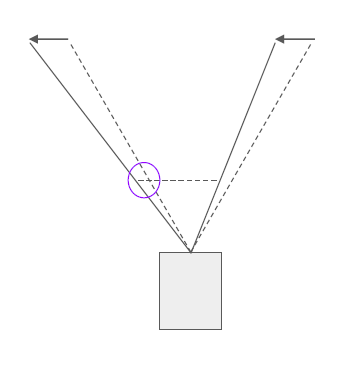
\includegraphics[scale=0.3]{images/camera_jitter.png}
	\caption{Proceso de \textit{Jittering} sobre la proyección de la cámara. Imagen tomada de la presentación de Fuglsand. \protect\cite{Fuglsand2016}}\label{fig:camerajittering}
\end{figure}

El \textit{Jittering} se aplica como una traslación a la matriz de proyección de la cámara usando la $Halton Sequence (2,3)$ (Secuencia de Halton) como los vectores de traslación. Esta secuencia se usa porque genera un patrón irregular para las traslaciones, que ayuda a conservar más información que un patrón regular y porque la Secuencia de Halton, proporciona un generador económico de patrones pseudoaleatorios. ~\cite{Fuglsand2016, XU2016}

\begin{figure}[!hbt]
	\centering
	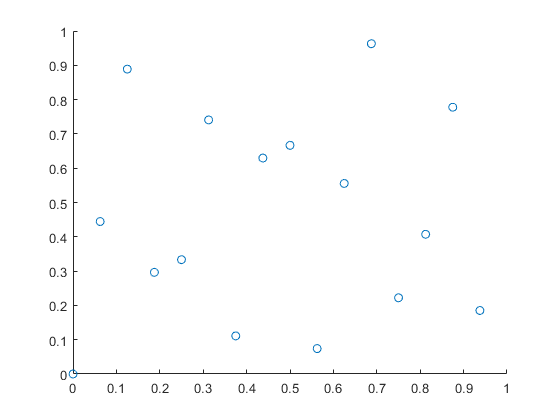
\includegraphics[scale=0.5]{images/halton_16.png}
	\caption{Valores usados de la $Halton Sequence (2,3)$ (Secuencia de Halton).}\label{fig:halton16}
\end{figure}

La Figura ~\ref{fig:halton16} muestra la representación de los 16 puntos utilizados para trasladar la proyección en la implementación actual de la tesis, tal como lo propusieron Fuglsand ~\cite{Fuglsand2016}. Los puntos se generaron usando MATLAB y luego se codificaron para mejorar su aleatoriedad usando reverse-radix scrambling.

\subsection{Buffer de Velocidad}
El algoritmo de Buffer de Velocidad (Velocity Buffer) utilizado en esta implementación es el propuesto por Chapman ~\cite{Chapman2012}, el cual es calculado restando la posición actual del píxel de su posición en el cuadro pasado. Esto es posible ya que guardamos la matriz que representa cada objeto en la escena y la utilizamos en el siguiente cuadro para calcular los píxeles del Buffer de Velocidad. Además, cancelamos matemáticamente el Cámara Jittering antes de calcular las velocidades, para evitar el ruido que crea, como lo sugiere Xu. ~\cite{XU2016}


\subsection{Buffer de Historia}
Para cada fragmento en el marco actual, buscamos en la vecindad de $3\times 3$ y en la vecindad del patrón Cruz $(+)$ alrededor de cada píxel (Ver figura ~\ref{fig:samplingpattern}). Buscamos en ambos patrones para el mínimo y el máximo de colores del cuadro actual, luego los promediamos y los usamos para construir parte del Color Clipping Box restringiendo los píxeles del Buffer de Historia. ~\cite{Fuglsand2016}
\begin{figure}[!hbt]
	\centering
	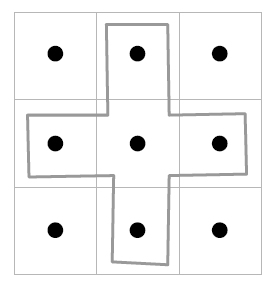
\includegraphics[scale=0.8]{images/sampling_pattern.png}
	\caption{Patrón de Muestreo utilizado. Imagen tomada de la presentación de Fuglsand. \protect\cite{Fuglsand2016}}\label{fig:samplingpattern}
\end{figure}

En la vecindad $3\times 3$ buscamos la velocidad del píxel con la profundidad más cercana a la cámara, esto es para obtener mejores bordes en movimiento para los píxeles que están ocultos detrás de otros ~\cite{Fuglsand2016}. Usamos esta velocidad para reproyectar la posición del píxel del cuadro actual en el Buffer de Historia. ~\cite{Fuglsand2016, XU2016}

Después de tener los píxeles en el Buffer de Historia, lo restringimos (explicación en la siguiente subsección) y lo interpolamos linealmente con el cuadro actual (Ver la Figura \ref{fig:samplingprocess} para obtener una representación visual del proceso completo). Interpolamos linealmente los píxeles del Buffer de Historia y el cuadro actual usando un valor de retroalimentación que se calcula por la diferencia de luminancia entre los colores del Buffer de Historia restringido y el cuadro actual. Este valor de retroalimentación es sesgado a favor de mantener el color del Buffer de Historia del píxel sobre el color del cuadro actual, esto se hace para agregar información del cuadro actual mientras se mantiene la mayor parte de la historia del píxel. Esta interpolación lineal estabiliza la imagen, eliminando el \textit{Jittering} y suavizando los bordes ~\cite{Fuglsand2016, XU2016}. Dado que el historial de cada píxel se acumula en el Buffer de Historia, obtenemos el efecto que el historial de píxeles de los cuadros anteriores pese menos cuanto más tiempo sea mantenido el historial del píxel dentro Buffer de Historia. ~\cite{Fuglsand2016}

\begin{figure}[H]
	\centering
	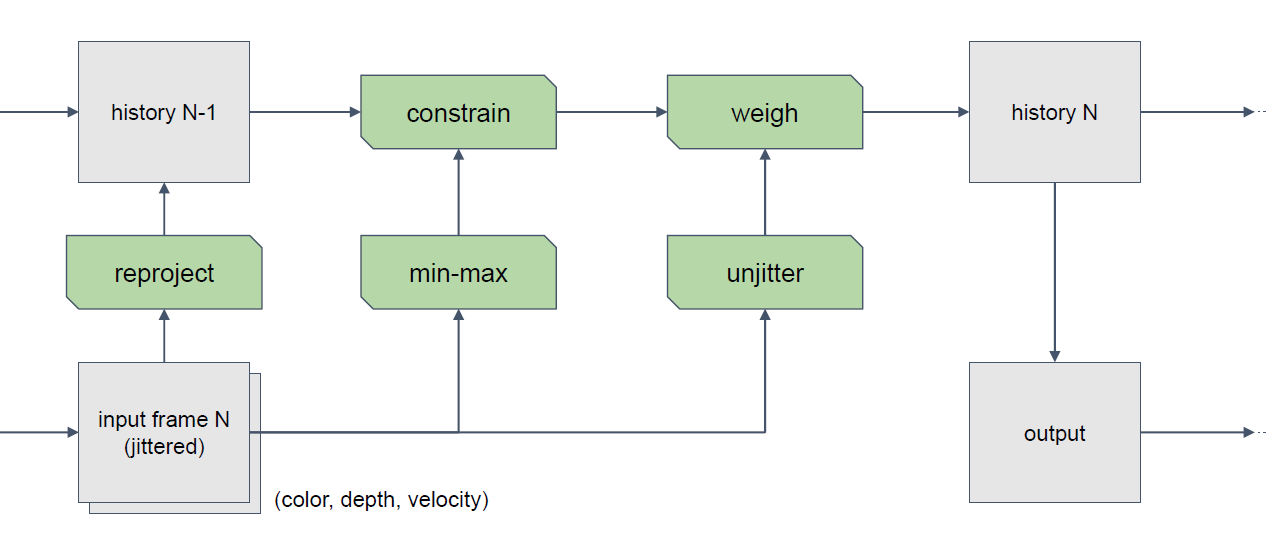
\includegraphics[scale=0.4]{images/sampling_process.png}
	\caption{Proceso de \textit{Temporal Reprojection Anti-Aliasing}. Imagen tomada de la presentación de Fuglsand \protect\cite{Fuglsand2016}}\label{fig:samplingprocess}
\end{figure}

\subsection{Clipping Color Box} 
La \textit{Clipping Color Box} (Caja de Recorte de Colores) a es una caja 3D construida utilizando el color de píxel actual como el centro y el color mínimo y máximo calculado en la última subsección como los límites. Se utiliza para manejar el rechazo de la historia, cuando el color del píxel en el Buffer de Historia está muy alejado del color actual. Tomamos el color de la historia como un vector y luego lo proyectamos contra los bordes de la caja; si se encuentra fuera del borde de la caja, mantenemos la proyección; de lo contrario, el color de la historia quedará intacto. El uso del Clipping Color Box evita la agrupación de colores en las esquinas que ocurriría si se aplicara \textit{clamping} (Ver Figura ~\ref{fig:clippingbox}). ~\cite{Fuglsand2016}.

\begin{figure}[!hbt]
	\centering
	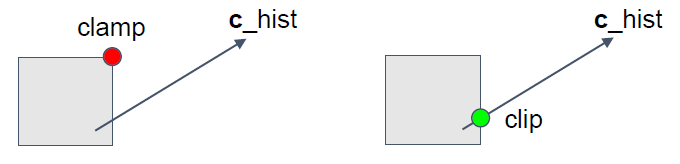
\includegraphics[scale=0.4]{images/clipping_box.png}
	\caption{\textit{Color Clamping} versus \textit{Color Clipping}. Imagen tomada del \textit{paper} de Fuglsand. \protect\cite{Fuglsand2016}}\label{fig:clippingbox}
\end{figure}


\subsection{Filtro de Nitidez} 
El Proceso de Reproyección y el \textit{Clipping} de Colores crean imágenes borrosas, por lo que se requiere un Filtro de Nitidez. Usamos el filtro propuesto por Xu. ~\cite{XU2016}

\begin{equation} \label{eq:sharpen}
\begin{bmatrix*}[r]
0 & -1 &  0 \\
-1 &  5 & -1 \\
0 & -1 &  0
\end{bmatrix*}
\end{equation}

La Ecuación \ref{eq:sharpen} representa la matriz de convolución utilizada como Filtro de Nitidez en el \textit{paper} de Xu. \protect\cite{XU2016}

\subsection{Motion Blur}
Debido a la naturaleza del Buffer de Historia, algo de \textit{ghosting} es creado por algunos fragmentos de objetos que se mueven más rápido que el tiempo que tarda el \textit{Clipping Color Box} para rechazar el color de píxeles antiguos, esto es especialmente notable bajo condiciones especiales de luz y fondo. Fuglsand y Xu ~\cite{Fuglsand2016, XU2016} propusieron usar soluciones como \textit{Motion Blur} para ocultar estos artefactos.

El \textit{Motion Blur} utilizado es el propuesto por Chapman ~\cite{Chapman2012}. Intenta comportarse como una cámara real, escalando la velocidad de cada píxel mediante la división de los cuadros actuales por segundo (FPS) a la velocidad deseada, simulando así la velocidad de obturación. Luego, mezcla los colores de los píxeles que se muestrean al seguir la dirección del vector del Buffer de Velocidad.


\subsection{Problemas}
Temporal Anti-Aliasing tiene dos inconvenientes principales, el efecto de Ghosting de los objetos en movimiento y el Desenfoque proveniente de la forma en que funciona el Clipping Color Box. Esta tesis pretende ayudar a reducir los efectos de estos dos inconvenientes utilizando nuevos enfoques. Por completitud, presentamos algunas de las soluciones actuales disponibles.

\subsubsection{Desenfoque} 
Las implementaciones actuales de TAA generan un desenfoque muy agresivo debido a la forma en que mezclan los colores del cuadro actual y el historial; el uso de áreas más grandes que el píxel aumenta los errores generados, por lo tanto, se requiere un Filtro de Nitidez. El filtro aplicado en la implementación es el utilizado por Xu ~\cite{XU2016}, que resuelve el desenfoque razonablemente bien, pero no logra eliminar algunos artefactos. 

\subsubsection{Ghosting} 
Algo de \textit{Ghosting} se crean cuando los objetos se mueven, especialmente bajo condiciones particulares de luz y fondo que hacen que el primer plano y el fondo se vean de manera similar. Esto se corrige parcialmente con \textit{Motion Blur}, sin embargo, parte de él permanece cerca de objetos que se mueven lo suficientemente rápido como para crear algo de \textit{Ghosting} pero lo suficientemente lentos como para evitar el \textit{Motion Blur}. Xu propone el uso de \textit{Motion Blur} y aumentar el tamaño de todo utilizando una técnica \textit{Stencil} y el etiquetado manual de objetos ~\cite{XU2016}, pero nuestro objetivo es evitar que los artistas etiqueten manualmente y prueben objetos por sus comportamientos bajo \textit{Ghosting}. La implementación de Pederson permite el \textit{Jittering} en los cálculos del Buffer de Velocidad para evitar \textit{Ghosting} en las imágenes, pero crea desenfoque no deseado. ~\cite{Fuglsand2016}. 

\section{Buffer de Acumulación}
El Buffer de Acumulación es una técnica de \textit{Anti-Aliasing} que consiste, según Paul Haeberli y Kurt Akeley \cite{Haeberli1990}, en renderizar la escena varias veces aplicando \textit{Jittering} a la cámara y luego realizar una suma ponderada a escala de las renderizaciones para generar el cuadro actual.

Este es un proceso que aumenta el muestreo por píxel y reduce los efectos de \textit{aliasing}, lo que produce una imagen de alta calidad a costa de procesar todo varias veces por cuadro.


\section{Operador de Sobel}
El Operador Sobel es un operador de gradiente isotrópico $3\times 3$ eficientemente computable, como lo explica Irwin Sobel \cite{Sobel2014}. Usamos este operador para detectar bordes en las imágenes renderizadas y marcarlos como posibles lugares con aliasing. Esto es porque son un lugar común para que aparezcan los artefactos de aliasing. 

Funciona al tomar las cuatro estimaciones de gradiente simple central posibles en un vecindario de $3\times 3$ y sumarlas. La función de imagen se toma como una función de densidad / intensidad y las cuatro posibles estimaciones como vectores ortogonales que son derivadas direccionales multiplicadas por un vector unitario que especifica la dirección de la derivada. La suma de las cuatro estimaciones posibles de gradiente simple central es equivalente a la suma vectorial de los ocho vectores derivativos direccionales.

\begin{equation}
\begin{bmatrix*}[r]\label{eq:sobel_neighborhood}
a & b & c \\
d & e & f \\
g & h & i
\end{bmatrix*}
\end{equation}

Sea la Matriz \ref{eq:sobel_neighborhood} sea Vecindario $3\times 3$ y $\abs*{G}$ la magnitud de la estimación derivada direccional del vecindario.

La dirección de $G$ estará dada por el vector unitario asociado al vecino apropiado. La suma vectorial hace que se cancelen todos los valores de $e$ (centro del  Vecindario $3\times 3$) dejando solo la siguiente expresión \ref{eq:sobel_simplification}:
\begin{equation}\label{eq:sobel_simplification}
\begin{split}
	G & =\frac{c-g}{4}*\begin{bmatrix*}1 & 1\end{bmatrix*}+\frac{a-i}{4}*\begin{bmatrix*}-1 & 1\end{bmatrix*}+\frac{b-h}{2}*\begin{bmatrix*}0 & 1\end{bmatrix*}+\frac{f-d}{2}*\begin{bmatrix*}1 & 0\end{bmatrix*} \\ & =\begin{bmatrix*}\frac{c-g-a+i}{4}+\frac{f-d}{2} & \frac{c-g+a-i}{4}+\frac{b-h}{2}\end{bmatrix*}
\end{split}
\end{equation}

Luego multiplicamos por $4$ para aproximar el valor y asegurarnos de que no perdamos precisión si lo realizamos con enteros pequeños de punto fijo. La magnitud recién calculada es dieciséis veces más grande que el gradiente promedio original.

\begin{equation}\label{eq:sobel_approximation}
\begin{split}
G' = 4 * G =\begin{bmatrix*}(c-g-a+i)+(f-d)*2 & (c-g+a-i)*4+(b-h)*2\end{bmatrix*}
\end{split}
\end{equation}

La Ecuación \ref{eq:sobel_approximation} se puede expresar en dos matrices de ponderación. Usamos la Matriz \ref{eq:sobel_x} para el componente $x$ y la Matriz \ref{eq:sobel_y} para el componente $y$.

\begin{equation}
\begin{bmatrix*}[r]\label{eq:sobel_x}
-1 &  0 & +1 \\
-2 &  0 & +2 \\
-1 &  0 & +1
\end{bmatrix*}
\end{equation}

\begin{equation}
\begin{bmatrix*}[r]\label{eq:sobel_y}
+1 & +2 & +1 \\
 0 &  0 &  0 \\
-1 & -2 & -1
\end{bmatrix*}
\end{equation}

Para la detección de bordes, lo que se hace comúnmente es comparar la magnitud de $G$ contra un umbral numérico para marcar píxels como bordes.

\section{Métricas de Imagen}
El proceso de medir la calidad de una imagen es complicado. Como explican Al-Najjar y Soong \cite{Yusra2012}, podemos seguir dos tipos métodos principales: subjetivo u objetivo. Los métodos subjetivos se basan en opiniones recogidas de humanos y, como cabría esperar, se consideran costosos, difíciles de implementar y llevan mucho tiempo. El segundo tipo de métodos, los objetivos, se basan en fórmulas matemáticas y algoritmos para medir la calidad de la imagen sin intervención humana. Para esta tesis, usamos métodos objetivos.

Los métodos de objetivos se pueden categorizar en tres grupos, como describen Al-Najjar y Soong \cite{Yusra2012}:

\begin{itemize}
	\item \textbf{Sin-Referencia:} En el cual no tenemos una imagen de referencia para comparar.
	\item \textbf{Referencia-Reducida:} Donde tenemos parte de una imagen de referencia.
	\item \textbf{Referencia-Completa:} Tenemos la imagen de referencia completa.
\end{itemize}


Para la computación gráfica, los métodos preferidos son los de Referencia-Completa porque las imágenes de referencia se pueden generar utilizando algoritmos de mayor calidad pero con mal rendimiento para representarlos. Las métricas más comunes utilizadas, y las utilizadas en esta tesis, son: Error Cuadrado Medio (MSE, \textit{Mean Square Error}); Relación Señal a Ruido de Pico (PSNR, \textit{Peak Signal-to-Noise Ratio}); y el Índice de Similitud Estructural  (SSIM, \textit{Structural Similarity Index}).

\subsection{Error Cuadrado Medio (MSE)}
Basada en el promedio del error cuadrado entre los píxeles de la imagen y la referencia. 

\begin{equation}\label{eq:mse}
	MSE=\frac{1}{N*M}\sum\limits_{i=0}^{N-1}\sum\limits_{j=0}^{M-1}(Im(i,j)-Ref(i,j))^2
\end{equation}
Donde $N, M$ son el ancho y largo de las imágenes y $Im, Ref$ son el píxel de la Imagen y la Referencia.

\subsection{Desviación de la Raíz Cuadrada Media  (RMSD)}
Es la desviación estándar de MSE (\textit{Root Mean Square Deviation}). También llamada \textit{Root Mean Square Error} (RMSE).
\begin{equation}\label{eq:rmse}
RMSE=\sqrt{MSE}
\end{equation}

\subsection{Relación Señal a Ruido de Pico (PSNR)}
Se basa en el concepto matemático de Relación de Señal a Ruido (SNR, Signal-To-Noise Ratio) que mide la señal de la imagen, que se almacena como los colores de los píxeles para nuestros propósitos, contra su error en comparación con la referencia. \cite{Yusra2012}

\begin{equation}\label{eq:psnr}
PSNR=10*\log\left(\frac{S^2}{MSE}\right)
\end{equation}

Donde $S$ es el valor máximo que puede alcanzar la señal. En nuestro caso es $255$ porque usamos canales de color de 8 bits.

\subsection{Índice de Similitud Estructural (SSIM)}
SSIM es una métrica de imagen ampliamente utilizada, que coincide con la subjetividad humana y es muy sensible a las degradaciones en la estructura espacial de la luminancia de la imagen, como explican Malpica y Bovik. \cite{Malpica2009}

Requiere dos imágenes para comparar, $X$ y $Y$, y se calcula en base a tres funciones de similitud en una ventana ponderada gaussiana de $N\times N$ (típicamente $11\times 11$).

\begin{equation}\label{eq:ssim_components}
\begin{split}
l(x,y) & = \frac{2*\mu_X(x,y)*\mu_Y(x,y)+C_1}{\mu_X^2(x,y)+\mu_Y^2(x,y)+C_1} \\ 
c(x,y) & = \frac{2*\sigma_X(x,y)*\sigma_Y(x,y)+C_2}{\sigma_X^2(x,y)+\sigma_Y^2(x,y)+C_2} \\ 
s(x,y) & = \frac{\sigma_{XY}(x,y)+C_3}{\sigma_X(x,y)+\sigma_Y(x,y)+C_3}
\end{split}
\end{equation}

Donde
\begin{equation*}
\begin{split}
\mu_X(x,y) & = \sum\limits_{p=-P}^{P} \sum\limits_{q=-Q}^{Q} w(p,q)*X(x+p,y+q)\\ 
\sigma_X^2(x,y) & = \sum\limits_{p=-P}^{P} \sum\limits_{q=-Q}^{Q} w(p,q)*\lbrack X(x+p,y+q)-\mu_X(x,y) \rbrack^2\\ 
\sigma_{XY}(x,y) & = \begin{split}\sum\limits_{p=-P}^{P} \sum\limits_{q=-Q}^{Q} w(p,q)& *\lbrack X(x+p,y+q)-\mu_X(x,y)\rbrack \\ & *\lbrack Y(x+p,y+q)-\mu_Y(x,y)\rbrack\end{split}
\end{split}
\end{equation*}

Donde $w(p, q)$ es una función de ponderación gaussiana tal que $\sum\limits_{p = -P}^{P}\sum\limits_{q = -Q}^{Q} w(p, q) = 1$ y $C_1, C_2, C_3$ son pequeñas constantes que proporcionan estabilidad cuando el denominador se aproxima a cero. Por lo general, se establecen de la siguiente manera: 
\begin{equation*}
	C_1=(K_1*L)^2,C_2=(K_1*L)^2,C_3=\frac{C_2}{2}
\end{equation*}

Donde $L$ es el rango dinámico de la imagen y $K_1, K_2 \ll1$ son pequeñas constantes. Al final, las tres funciones de similitud se combinan en la forma general:

\begin{equation}\label{eq:ssim}
SSIM(x,y)=l(x,y)*c(x,y)*s(x,y)
\end{equation}



\chapter{Desarrollo}
En este capítulo, se presenta el trabajo principal realizado en esta tesis.
\section{Mejoras al Proyecto de EDAN35}
Para esta tesis, decidimos utilizar nuestro proyecto de \textit{High Performance Computer Graphics} (EDAN35) como base. Durante el curso implementamos una técnica de \textit{Temporal Reprojection Anti-Aliasing} (TRAA, Anti-Aliasing de Reproyección Temporal) basada en las presentaciones de Ke Xu y Lasse Fuglsang ~\cite{XU2016, Fuglsand2016}, de los juegos \textit{Inside} y \textit{Uncharted 4}. Esta resultó ser confiable y bien documentada; y nos permitió poner en práctica los fundamentos de la técnica en un entorno académico, proporcionando la base para las mejoras realizadas para esta tesis.

La implementación del proyecto EDAN35 tenía errores en el Proceso de \textit{Jittering} que se corrigieron al expandir correctamente en lo que ambas implementaciones se referían por \textit{Jittering} de Cámara, consulte el Apéndice \ref{appendix:jitter} para obtener una explicación completa. El manejo de los puntos de \textit{Halton} se rehizo para lograr la mejora del movimiento de la cámara, se incluyó el soporte de hasta 128 puntos para que funcione como el \textit{Jittering} del Buffer de Acumulación (Ver Figura \ref{fig:halton128}). Sin embargo, hay que tener en cuenta que para el \textit{Temporal Anti-Aliasing}, solo los primeros 16 puntos se usan según lo sugerido por Xu y Fuglsang. ~\cite{XU2016, Fuglsand2016}

\begin{figure}[!hbt]
	\centering
	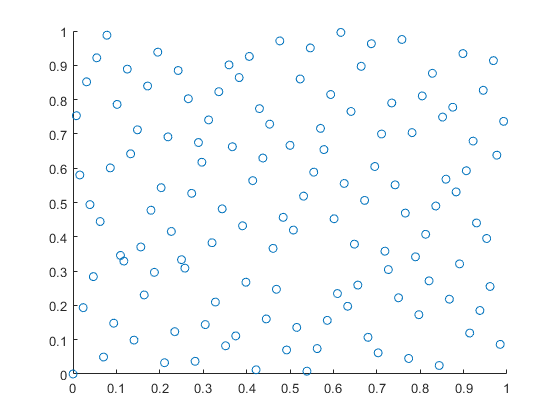
\includegraphics[scale=0.5]{images/halton_128.png}
	\caption{Los $128$ de la $Secuendia Halton (2,3)$ disponibles para usar.}\label{fig:halton128}
\end{figure}

El \textit{Anti-Aliasing} de Iluminación Especular, como superficies metálicas, es un problema complejo en sí mismo que requiere soluciones especializadas que funcionen directamente con los reflejos de la luz. Las técnicas \textit{Anti-Aliasing} no lo corrigen este problema por sí mismas, generalmente funcionan en conjunto con soluciones adecuadas ya hechas. Por esto, para evitar problemas con la iluminación especular, se decidió apagarla.

Además, se agregaron modelos de una esfera, pared, tubería, \textit{Hairball} (Bola de Pelo), una ventana con persianas y una ventana arqueada para probar las mejoras realizadas al \textit{Temporal Anti-Aliasing}. Todos los modelos, excepto la pared, se agregaron con una textura de color sólido para evitar la introducción de errores de iluminación en los cálculos de las métricas de imagen, ya que estas son usadas para las comparaciones entre la implementación de Uncharted 4 y la desarrollada en esta tesis. El modelo de la pared usa una textura blanca con letras negras, porque las letras usan bordes duros para definir su forma y debe permanecer así después de aplicar cualquier técnica de \textit{Anti-Aliasing}.

\subsection{Fast Approximate Anti-Aliasing (FXAA)}
Para esta tesis, se usó la versión del \textit{white paper} (paper inicial) de \textit{Fast Approximate Anti-Aliasing} (FXAA, \textit{Anti-Aliasing} Aproximado Rápido) de Lottes \cite{Lottes2009} para compararla con \textit{Temporal Anti-Aliasing}, basándose en que ambas técnicas son \textit{Anti-Aliasing} y post-procesamiento, y que FXAA es una técnica popular utilizada en la industria. Esta técnica se implementó bajo el preajuste de mayor calidad según el \textit{white paper} sin tener en cuenta el impacto en el rendimiento porque queríamos comparar la mejora cruda que ambas técnicas pueden proporcionar.

\subsection{Enhanced Subpixel Morphological Antialiasing (SMAA)}
Con el fin de probar una técnica de post-procesado más compleja y más nueva, se implementó SMAA siguiendo las instrucciones proporcionadas por Jiménez et al \cite{Jimenez2012}. Se utilizó el valor preestablecido más alto que funciona con la Arquitectura de \textit{Shading} Diferido.

\subsection{Buffer de Acumulación}
Usamos un Buffer de Acumulación para proporcionar una imagen de referencia de la escena. Fue implementado siguiendo a Haeberli y Akeley \cite{Haeberli1990}. Los puntos usados para realizar \textit{jittering} a la cámara son los mismos puntos de la Secuencia de Halton que usa \textit{Temporal Anti-Aliasing}, aunque el Buffer de Acumulación puede usar hasta 128. Las razones para usar la Secuencia de Halton son las siguientes: cumple con los requisitos establecidos por Haeberli y Akeley; es fácil ampliar el sistema de cámara actual para admitir más puntos Halton; e, igual que para \textit{Temporal Anti-Aliasing}, proporciona puntos pseudoaleatorios que no siguen un patrón para ayudar a reunir tanta información de la escena como sea posible.

\subsubsection{Número de Muestras Seleccionadas}
El número de muestras seleccionadas para el Buffer de Acumulación es 128. Esto se debe a que proporciona la mejor representación posible de la escena a pesar de que causa una pérdida sustancial de rendimiento.

Para mostrar la diferencia entre el uso de 16 y 128 muestras, realizamos cuatro pruebas, denominadas de A a D, para observar cómo se comportan las medidas bajo diferentes arreglos de objetos e iluminación en la escena. En la tabla \ref{tab:acctest} vemos los resultados de una de esas pruebas:

\begin{table}[!hbt]
	\centering
	\caption{Comparación del comportamiento de las métricas entre el uso de 16 muestras frente a 128 para el Buffer de Acumulación.}\label{tab:acctest}
\begin{tabular}{ | l | c | c | c | c | }
	\hline
	\multicolumn{5}{| c |}{\textbf{Prueba D}} \\
	\hline
	\textbf{\diagbox{Pruebas}{Muestras}}  & \textbf{\makebox{16}} & \textbf{\makebox{128}} & \textbf{\makebox{Diferencia}} & \textbf{\makebox{Diferencia Relativa $(\%)$}} \\
	\hline
	MSE de Temporal	& $40.647863$ & $38.947297$	& $-1.700566$ & $4.183654132\%$ \\
	\hline
	RMSD de Temporal & $6.375568$ & $6.240777$ & $-0.134791$ & $2.114180258\%$ \\
	\hline
	MSE de No AA & $24.872104$ & $24.524992$ & $-0.347112$ & $1.395587603\%$ \\
	\hline
	RMSD de No AA & $4.987194$ & $4.952271$ & $-0.034923$ & $0.700253489\%$ \\
	\hline
	Peak-SNR de Temporal & $32.040426$ & $32.22603$ & $0.185604$ & $0.575944353\%$ \\
	\hline
	SNR de Temporal & $30.30596$ & $30.492374$ & $0.186414$ & $0.611346299\%$ \\
	\hline
	Peak-SNR de No AA & $34.173678$ & $34.234715$ & $0.061037$ & $0.178289786\%$ \\
	\hline
	SNR de No AA & $32.439212$ & $32.501058$ & $0.061846$ & $0.190289190\%$ \\
	\hline
	SSIM de Temporal & $0.993302$ & $0.993451$ & $0.000149$ & $0.014998223\%$ \\
	\hline
	SSIM de No AA & $0.996826$ & $0.996891$ & $6.5E-05$ & $0.006520272\%$ \\
	\hline		
\end{tabular}
\end{table}

Los cambios son lo suficientemente grandes en algunas métricas para ser perceptibles, especialmente en MSE y SSIM de Temporal Anti-Aliasing para nuestras comparaciones entre técnicas \textit{Anti-Aliasing}. Vamos a notar los efectos del uso de 128 muestras cuando lleguemos a las comparaciones entre las técnicas \textit{Anti-Aliasing}.

\section{Implementación del Marco de Pruebas}
Para medir cualquier mejora lograda, desarrollamos un marco de prueba que nos permite guardar la información importante cuando se realiza una prueba. El marco nos permite seleccionar qué técnica utilizar como el renderizador principal: la implementación de \textit{Temporal Anti-Aliasing} de la Tesis, \textit{Temporal Anti-Aliasing} de \textit{Uncharted 4},  Enhanced Subpixel Morphological Anti-Aliasing (SMAA) o \textit{Fast Approximate Anti-Aliasing} (FXAA). También nos permite hacer zoom en cualquier parte de la pantalla y luego realizar todos los cálculos de métricas de imágenes usando MATLAB.

Cuando se realiza una prueba, las imágenes renderizadas seleccionadas se guardan como PNG’s con 4 canales de color y sin compresión. Además, información básica sobre la fecha en que se realizó la prueba, la información de la cámara y los datos de a los valores utilizados para el \textit{Temporal Anti-Aliasing} se guardan en un archivo de texto sin plano.

Para cuantificar si se lograron los objetivos propuestos de esta tesis, sobre \textit{ghosting} y desenfoque, desarrollamos dos tipos diferentes de pruebas: Pruebas Estáticas y Pruebas de \textit{Ghosting}.

\subsection{Pruebas Estáticas}
Este tipo de prueba consiste en dejar que el Buffer de Historia se llene de 16 cuadros de la escena, sin ningún objeto en movimiento, utilizando la técnica \textit{Temporal Anti-Aliasing} seleccionada para luego guardar el último cuadro renderizado. Inmediatamente después de guardar el último cuadro de TAA, renderizamos el último cuadro nuevamente pero ahora utilizando el Buffer de Acumulación, para generar la imagen base de la escena. También, renderizamos el último cuadro usando SMAA, FXAA y \textit{No Anti-Aliasing} (NOAA, No AA), para propósitos de comparación.

\subsection{Pruebas de Ghosting}
Este tipo de prueba se realiza solo con los modelos de la Esfera y \textit{HairBall}; el primero se mueve a través del pasillo de la escena, simulando un objeto en movimiento en una aplicación, y el segundo gira en una posición estática, simulando muchos bordes en movimiento. La prueba consiste en renderizar la escena por un número seleccionado de cuadros, con la implementación de la Tesis de \textit{Temporal Anti-Aliasing} y la implementación de Uncharted 4 de \textit{Temporal Anti-Aliasing} al mismo tiempo. Después de renderizar cada cuadro, se guardan cada imagen, la posición de la esfera y la rotación de \textit{Hairball}

Una vez que el número seleccionado de cuadros se ha renderizado, la esfera vuelve a su posición original y el movimiento se repite utilizando las posiciones guardadas anteriormente. \textit{Hairball} también vuelve a su rotación original y el movimiento también se repite. La diferencia esta vez es que cada cuadro se procesa utilizando el Buffer de Acumulación y luego se guarda, se hace para evitar la gran pérdida de rendimiento causada, que afecta las técnicas de \textit{Temporal Anti-Aliasing}.

Después de guardar todas las imágenes renderizadas, comparamos las producidas por el \textit{Temporal Anti-Aliasing} de la Tesis y el \textit{Temporal Anti-Aliasing} de Uncharted 4 contra la imagen base para calcular las métricas de la imagen de ellos. Estas métricas muestran cuánto error se generó por efecto de \textit{ghosting} en ambas implementaciones, lo que nos permite comparar cómo se comportan ambas técnicas. 


\subsection{Métricas de Imagen de MATLAB}
Las métricas de las imágenes para cada prueba representan, numéricamente, la calidad de cada imagen. Los calculamos para comparar cómo se comportó cada técnica en cada prueba para identificar si el \textit{Temporal Anti-Aliasing} de la Tesis genera imágenes de mayor calidad que las otras técnicas probadas.

Una vez que se guardan todos los resultados de la prueba, una secuencia de comandos toma todas las imágenes y las organiza en carpetas por nombre y tipo de prueba. Después, todos los resultados de la prueba se procesan utilizando MATLAB para obtener los resultados de las métricas de las imágenes. Con los resultados de las métricas de imagen, comparamos cómo se comportó el \textit{Temporal Anti-Aliasing} de la Tesis con el \textit{Temporal Anti-Aliasing} de Uncharted 4 y las otras técnicas \textit{Anti-Aliasing}, para detectar si las mejoras funcionaban y observar cómo se comportó nuestra implementación mejorada frente a las demás.

Para las Pruebas Estáticas, realizamos mediciones de MSE, RMSD, PSNR, SNR y SSIM en las imágenes renderizadas de TAA, FXAA, SMAA y No AA, utilizando las imágenes renderizadas del Buffer de Acumulación como referencia para comparar. Asimismo, generamos un mapa local de SSIM para cada imagen renderizada, además del renderizado con el Buffer de acumulación, que se guardan como PNGs y FIGs de MATLAB. Todos los resultados de las mediciones se almacenan en la carpeta con los resultados de la prueba como texto plano.

Para Pruebas de Ghosting, realizamos mediciones de MSE, RMSD, PSNR, SNR y SSIM en cada cuadro procesado con la técnica de Temporal Anti-Aliasing de Uncharted 4 y el Temporal Anti-Aliasing de la Tesis, utilizando el cuadro renderizado del Buffer de Acumulación correspondiente. Se genera un mapa local de SSIM para cada imagen renderizada, exceptuando las del Buffer de Acumulación, y se guardan como PNG y FIGs de MATLAB. Todos los resultados de todas las imágenes se almacenan en un archivo de texto plano. En los mapas locales de SSIM, las diferencias son representadas como colores, el blanco simbolizando la similitud.


\section[Modificaciones de Temporal Reprojection Anti-Aliasing ]{Modificaciones de Temporal Reprojection Anti-Aliasing }
Para esta tesis, la técnica del \textit{Color Clipping Box} se modificó para que se viera afectada por los valores calculados a partir de las nuevas técnicas aplicadas en esta tesis. Estos cambios siguen la lógica de que queremos aplicar toda la fuerza de la técnica de \textit{Temporal Anti-Aliasing} cuando sea necesario y minimizar la aplicación de la técnica en otras partes, para minimizar los efectos de la \textit{ghosting} y el desenfoque.

El primer cambio consiste en que los colores que se calcularon a partir del promedio entre las vecindades $3\times 3$ y Cruz, de los patrones de muestreo (ver Figura \ref{fig:samplingpattern_2}), ahora se mezclan en una cantidad variable. Esto sigue la idea de que preferimos la vecindad de Cruz si el píxel que estamos calculando actualmente no se considera con \textit{aliasing}, porque es menos probable que la vecindad de Cruz introduzca ruido en los cálculos de la \textit{Color Clipping Box}. Pero, si se considera que el píxel con \textit{aliasing}, preferimos el vecindario $3\times 3$ porque proporciona más información sobre el entorno del píxel para crear la imagen sin \textit{aliasing}. 

\begin{figure}[!hbt]
	\centering
	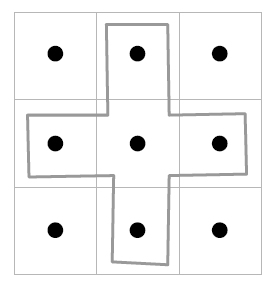
\includegraphics[scale=0.3]{images/sampling_pattern.png}
	\caption{Patrón de muestreo utilizado. Imagen tomada de la presentación de Fuglsand. \protect\cite{Fuglsand2016}}\label{fig:samplingpattern_2}
\end{figure}

El segundo cambio consiste en que el tamaño de la \textit{Color Clipping Box} depende de cuánto \textit{aliasing} se considera que el píxel tiene. Al utilizar \textit{Color Clipping Box} más pequeñas (Ver Figura \ref{fig:colorclippingboxredux}) que la técnica original en píxeles sin \textit{aliasing}, aumentamos la eliminación de colores no deseados del historial, reduciendo los efectos del efecto \textit{ghosting} ya que rechazamos colores más rápido en píxeles que sabemos que no se consideran con aliasing. Esto se implementa mediante la interpolación lineal del color de píxel actual y los colores mínimo y máximo calculados para construir la \textit{Color Clipping Box}.

\begin{figure}[!hbt]
	\centering
	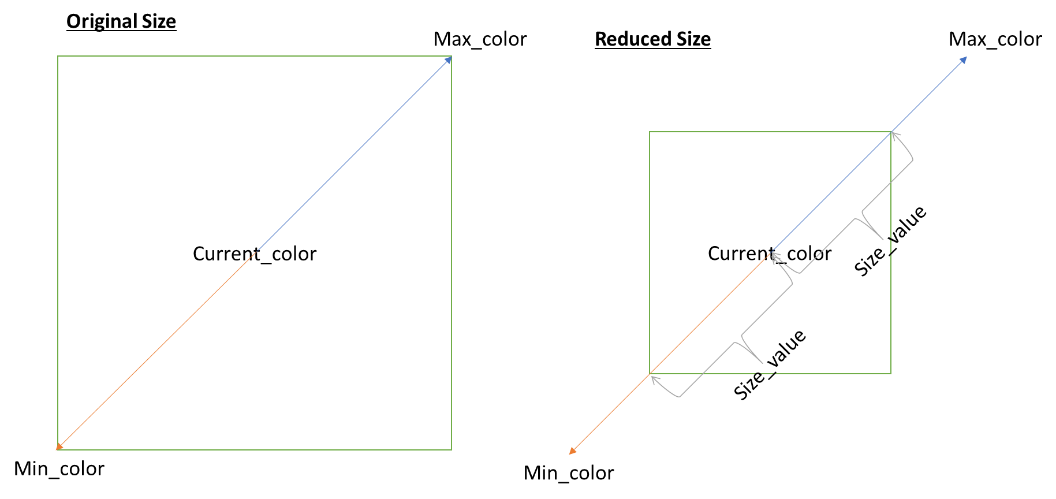
\includegraphics[scale=0.3]{images/clipping_box_reduction.png}
	\caption{Reducción de tamaño de la Color Clipping Box}\label{fig:colorclippingboxredux}
\end{figure}

En las siguientes subsecciones, explicaremos cómo se calculan todos los valores que contribuyen a decidir si un píxel se considera con \textit{aliasing} o no. Todos estos valores se calculan al mismo tiempo que se aplica TAA, con la excepción del Operador de Sobel, que ocurre antes de la técnica TAA principal. Después, mostramos cómo usamos ese valor para reducir el tamaño del \textit{Color Clipping Box} y la preferencia del patrón de muestreo.

\subsection{Implementación de Mejoras de Indexación de Triángulos}
La idea principal detrás de la aplicación de esta técnica es detectar los píxeles que consideramos con \textit{aliasing} utilizando la cantidad de modelos diferentes que rodean a un píxel. Queremos detectar los bordes entre diferentes modelos porque el \textit{aliasing} normalmente ocurre allí. Una vez que tenemos esta información, procedemos a modificar la \textit{Color Clipping Box} que controla la aplicación de TAA.

Para implementar esta técnica, todos los modelos en la escena reciben un índice único. Luego, en el pase de Renderización de Geometría, todos los triángulos que pertenecen a un mismo modelo reciben el índice del modelo como su ID. Posteriormente, se usa en el \textit{píxel shader} para generar una textura en la que cada píxel contiene el ID del modelo al que pertenece.

En el pase de Reproyección Temporal, se calcula el promedio del número de píxeles pertenecientes a diferentes modelos en la vecindad $3\times 3$ del píxel siendo revisado. Con este promedio, procedemos a sesgar la interpolación lineal de color entre el mínimo, máximo y promedio entre las vecindades Cruz y $3\times 3$ del píxel y procedemos a cambiar el tamaño del \textit{Color Clipping Box}.

Si el promedio es cercano a cero, lo que significa que el píxel está rodeado por píxeles de su mismo modelo, interpolamos hacia los colores de la vecindad Cruz y reducimos el tamaño de la \textit{Color Clipping Box}. Pero, si el promedio es cercano a uno, lo que significa que el píxel está rodeado por muchos píxeles de otros modelos, interpolamos hacia los colores de la vecindad $3\times 3$ y dejamos que la \textit{Color Clipping Box} permanezca en su tamaño original.

\begin{equation}\label{eq:model_index_acc}
modelAverage_i = \frac{\sum\limits_{j=1}^{9} ModelDiff(i,j)}{9} 
\end{equation}

Donde
\begin{equation*}
ModelDiff(i,j) = \left\lbrace \begin{split}1\quad & if\quad ModelID_i \neq ModelID_j \\ 0\quad & else\end{split} \right.
\end{equation*}

A continuación, vamos a mostrar algunos ejemplos de cómo funciona esta técnica. Para cada matriz, los números representan los ID’s de los triángulos, siendo la posición central el píxel que actualmente se está calculando y el resto siendo su vecindad. La Matriz \ref{eq:triang_index_not_aliased} muestra un ejemplo de un píxel no considerado con \textit{aliasing} porque la mayoría de sus vecinos tienen el mismo ID. Por otro lado, la Matriz \ref{eq:triang_index_aliased} muestra un pixel considerado con \textit{aliasing} debido a la gran cantidad de ID’s diferentes alrededor.

\begin{equation}
\begin{bmatrix*}[r]\label{eq:triang_index_not_aliased}
3 &  3 & 3 \\
3 &  3 & 3 \\
5 &  23 & 82
\end{bmatrix*}
\end{equation}

\begin{equation}
\begin{bmatrix*}[r]\label{eq:triang_index_aliased}
3 &  3 & 3 \\
3 &  5 & 3 \\
5 &  23 & 82
\end{bmatrix*}
\end{equation}

\subsection{Pseudo-Varianza de Profundidad y Pseudo-Varianza Temporal de Profundidad}
La razón detrás de esta técnica es que queremos detectar píxeles que están en una vecindad de píxeles separados por profundidades relativamente largas. También, queremos detectar píxeles cuya profundidad en el último cuadro cambió, relativamente, una distancia larga en contraste con su vecindad actual. Todos los píxeles que detectamos los consideramos con \textit{aliasing}.

Primero, calculamos la profundidad lineal mínima, máxima y su promedio del vecindario $3\times 3$. Luego procedemos a usar la siguiente fórmula para calcular el valor que vamos a usar para normalizar los resultados: 
\begin{equation} \label{eq:maxdepthdistance}
\begin{split} 
	maxDepthDistance = min \left( \right. & \left| depthMin-depthAvg \right|  ,   \\ 
	 &  \left.\left| depthMax-depthAvg\right| \right) 
\end{split} 
\end{equation}

Calculamos el valor de normalización utilizando el mínimo para evitar la interferencia de valores atípicos. Si $maxDepthDistance$ está por debajo de $0.002$, todo lo que sigue se establece en cero porque los píxeles están tan cerca que probablemente no tengan aliasing. Este umbral se definió experimentando qué valores no generan ruido dentro de los cálculos, pero dejan entrar los píxeles interesantes.

Luego calculamos la Pseudo-Varianza de Profundidad como:

\begin{equation} \label{eq:depthpseudovariance}
	depthPseudoVariance = \left( \frac{\left|currentDepth-depthAvg\right|}{maxDepthDistance}\right)^2
\end{equation}

Esto nos proporciona una Pseudo-Varianza que mide la distancia entre la profundidad promedio de la vecindad y la profundidad actual del píxel. Hay que tener en cuenta que normalmente el valor va a ser entre $0$ y $1$ pero, si la profundidad del píxel es un valor atípico en la vecinda, este valor va a ser superior a $1$.

Finalmente, calculamos cómo la profundidad del píxel en el último cuadro se relaciona con la vecindad actual, usando la Pseudo-Varianza Temporal de Profundidad. Hay que tener en cuenta que usamos la cuarta potencia para reducir el ruido en los cálculos; dado que el valor normalizado está entre $0$ y $1$, esto lo hace converger a $0$ si el valor era cercano a $0$ o a $1$ si es cercano a $1$.

\begin{equation} \label{eq:depthtemporalpseudovariance}
depthTemporalPseudoVariance = \left( \frac{\left|pastDepth-depthAvg\right|}{maxDepthDistance}\right)^4
\end{equation}

A continuación, vamos a mostrar ejemplos de cómo esta técnica decide si un píxel se considera con aliasing o no. Para cada matriz, los números representan las profundidades de los triángulos, siendo la posición central el píxel actual que se analiza y el resto es su vecindad. La Matriz \ref{eq:depth_var_not_aliased} nos muestra un ejemplo de un pixel no considerado con aliasing porque está relativamente cerca de la mayoría de sus vecinos. Por el contrario, la Matriz \ref{eq:depth_var_aliased} muestra un ejemplo de un píxel que se consideraría con aliasing porque tiene una distancia relativamente grande en comparación con su vecindad. Un ejemplo de un píxel considerado con aliasing por la Pseudo-Varianza Temporal de Profundidad, sería si la profundidad del píxel de la Matriz \ref{eq:depth_var_not_aliased} en el último cuadro fuera de $4.0$.

\begin{equation}\label{eq:depth_var_not_aliased}
\begin{bmatrix*}[r]
9.0 &  9.3 & 8.7 \\
9.2 &  9.0 & 9.3 \\
8.8 &  8.9 & 8.7
\end{bmatrix*}
\end{equation}

\begin{equation}\label{eq:depth_var_aliased}
\begin{bmatrix*}[r]
9.0 &  9.3 & 8.7 \\
9.2 &  4.0 & 9.3 \\
8.8 &  8.9 & 8.7
\end{bmatrix*}
\end{equation}

\subsection{Implementación de las Mejoras de Sobel}
La idea principal detrás de la aplicación de la técnica de detección de bordes de Sobel es concentrar los efectos TAA en píxeles en los bordes para corregir el \textit{aliasing}, si es necesario. Es importante señalar que esta es la única técnica de las mejoras de la tesis que se ejecuta antes del algoritmo TAA principal.

Aplicamos el Operador Sobel a la luminancia de los colores de la escena iluminada producida por la Arquitectura de \textit{Shading} Diferido, la luminancia de los colores de la escena no iluminada del Buffer de Geometría y la profundidad lineal actual. Utilizamos la luminancia porque el ojo humano reconoce mejor los cambios repentinos y usamos la escena, iluminada y no iluminada, para evitar problemas al detectar bordes debido a luces o sombras.

Cada operador de Sobel se realiza por separado, y sus magnitudes se mezclan al final de la siguiente manera:
\begin{equation} \label{eq:sobel_g}
	g=(u*0.3 +l*0.7)+d 
\end{equation}

Donde $u$ es la magnitud del Operador Sobel de la luminancia de la escena no iluminada, $l$ es la magnitud del Operador Sobel de la luminancia de la escena iluminada y $d$ es la magnitud del Operador Sobel de la profundidad lineal actual. \\

Luego, restringimos(\textit{clamp}) $g$ entre $0.0$ y $1.0$ para finalmente aplicar el polinomio de paso suave (\textit{smoothstep}) de la siguiente manera:
\begin{equation} \label{eq:sobel_sqrt}
sobel=\sqrt{g^2*(3.0-2.0*g)} 
\end{equation}

Después de aplicar todos los Operadores de Sobel, guardamos los resultados en una textura y realizamos una versión simplificada de TRAA para mantener los resultados estables a lo largo del tiempo. Esta versión simplificada es casi la misma que la que usamos como base de esta tesis, las diferencias provienen del uso de \textit{Clamping} (Restricción) en lugar de una \textit{Color Clipping Box}, porque los valores de textura son unidimensionales; y que no aplicamos un Filtro de Nitidez.

La salida de este TRAA se usa para calcular el valor de Sobel del píxel actual, el valor promedio de Sobel en la Vecindad Cruz y el valor promedio de Sobel en la Vecindad $3\times 3$.

\subsection{Mezcla Final}
Finalmente, modificamos cómo se calcula la \textit{Color Clipping Box} utilizando los valores que calculamos previamente. Llamamos a este valor mezclado final $aliasedValue$, el cual representa la cantidad de un pixel que se considera con \textit{aliasing}. Después de calcularlo, lo usamos para cambiar el patrón de muestreo a partir del cual se construye la \textit{Color Clipping Box} y su tamaño.

Primero, definimos la función de mezcla de la siguiente manera:
\begin{equation} \label{eq:mixfunction}
Mix(x,y,t)=x*(1-t)+y*t\quad with\; 0\leq t\leq 1
\end{equation} 

Luego, la mezcla final se aplica de la siguiente manera:
\begin{equation}\label{eq:sobelavgmixval}
sobelAvgMixVal=Clamp01(modelAverage_i+sobel) 
\end{equation}
 
Donde $sobel$ es el valor Sobel del píxel actual, de la Ecuación \ref{eq:sobel_sqrt}, $modelAverage_i$ proviene de la Ecuación \ref{eq:model_index_acc} y $Clamp01$ es la función de Clamping (Restricción) entre $0$ y $1$. \\

\begin{equation}\label{eq:sobelavg}
sobelAvg=Mix(sobelAvgCross, sobelAvg3x3, sobelAvgMixVal)
\end{equation}

Donde $sobelAvgCross$ es el valor promedio de Sobel de la Vecindad Cruz y $sobelAvg3x3$ es el valor promedio de Sobel de la Vecindad $3\times 3$ alrededor del píxel actual. \\ 

Y, utilizamos las Ecuaciones \ref{eq:sobelavg}, \ref{eq:depthpseudovariance}, \ref{eq:depthtemporalpseudovariance} y \ref{eq:model_index_acc} para calcular cuánto \textit{aliasing} se considera este píxel tiene:
\begin{equation}\label{eq:aliasedvalue}
\begin{split}
aliasedValue=Clamp01 (& sobelAvg + depthPseudoVariance \\
 & + depthTemporalPseudoVariance \\
 & + modelAverage_i)
\end{split}
\end{equation}

Con este $aliasedValue$ (valor de \textit{aliasing}) procedemos a modificar la \textit{Color Clipping Box}. Primero, seleccionamos cuánto de cada patrón de muestreo queremos que sea parte del \textit{Color Clipping Box}:
\begin{equation}\label{eq:newcolors}
\begin{split}
colorMin= & Mix(colorMinCross,colorMin3x3,aliasedValue) \\
colorMax= & Mix(colorMaxCross,colorMax3x3,aliasedValue) \\
colorAvg= & Mix(colorAvgCross,colorAvg3x3,aliasedValue) \\
\end{split}
\end{equation}

Luego modificamos el tamaño del \textit{Color Clipping Box} mediante la interpolación hacia el tamaño normal si el $aliasedValue$ está cerca de uno; en caso contrario, usamos el color actual, que es el centro del cuadro, lo cual disminuye el tamaño.
\begin{equation}\label{eq:clipredux}
\begin{split}
	clipColorMin= & Mix(colorCurrent,colorMin,aliasedValue) \\
	clipColorMax= & Mix(colorCurrent,colorMax,aliasedValue)
\end{split}
\end{equation}



Las Figuras \ref{fig:aliasedval1}, \ref{fig:aliasedval2} y \ref{fig:aliasedval3} son ejemplos de los valores de \textit{aliasing} calculados, cada píxel representa el $aliasedValue$ actual de esa imagen. El color blanco representa un $aliasedValue$ de $1$ y el color negro de $0$. Como esperamos, la mayoría de los bordes están marcados como probablemente con \textit{aliasing} por las técnicas que utilizamos.

\begin{figure}[H]
	\centering
	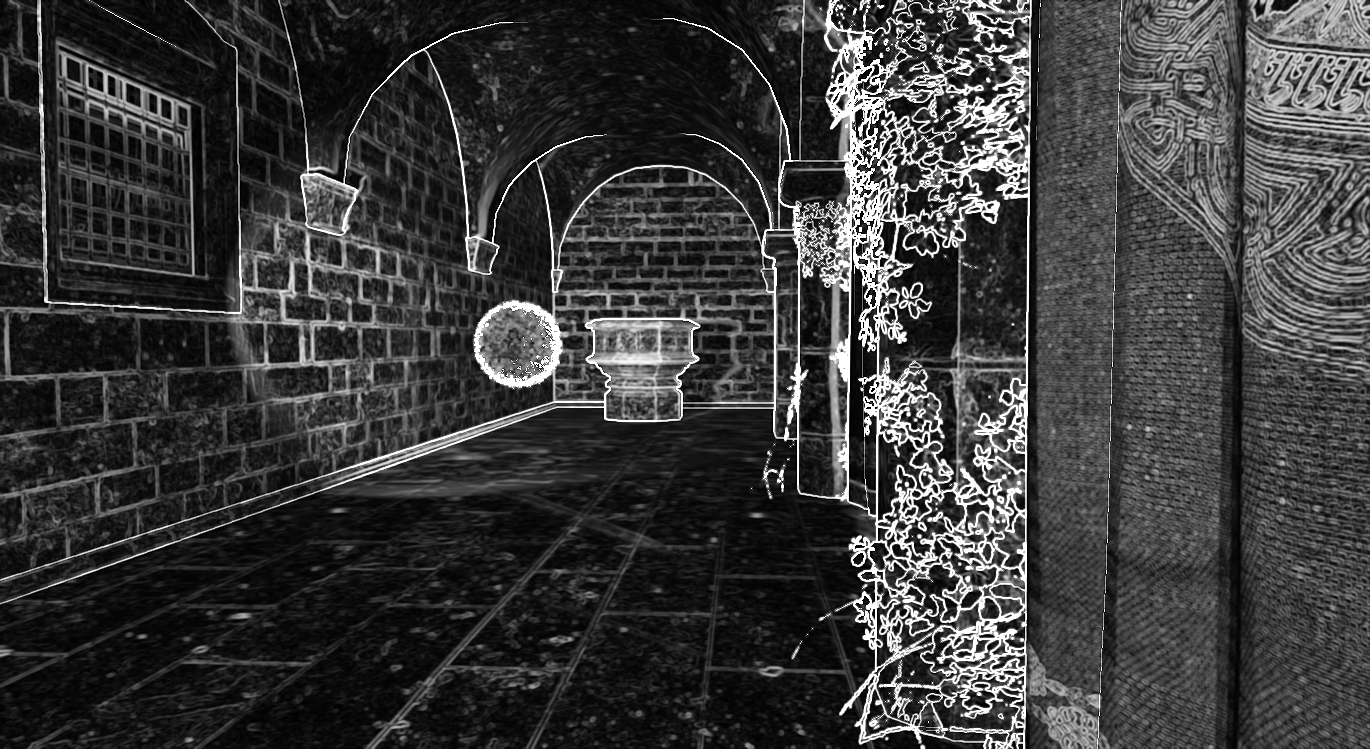
\includegraphics[scale=0.2]{images/aliased_value_example_1_temporal.png}
	\caption{Imagen hecha de los valores de \textit{aliasing} de cada píxel.}\label{fig:aliasedval1}
\end{figure}

\begin{figure}[H]
	\centering
	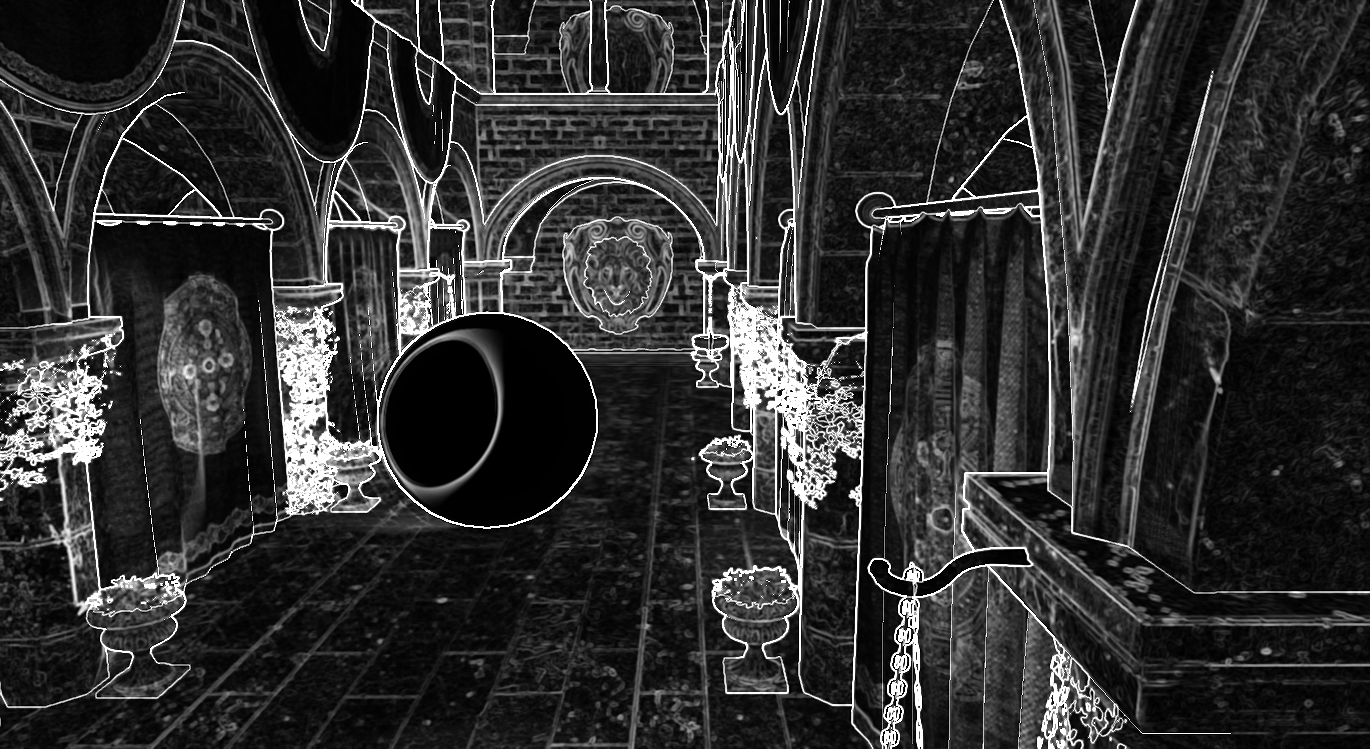
\includegraphics[scale=0.2]{images/aliased_value_example_2_temporal.png}
	\caption{Imagen hecha de los valores de \textit{aliasing} de cada píxel.}\label{fig:aliasedval2}
\end{figure}

\begin{figure}[H]
	\centering
	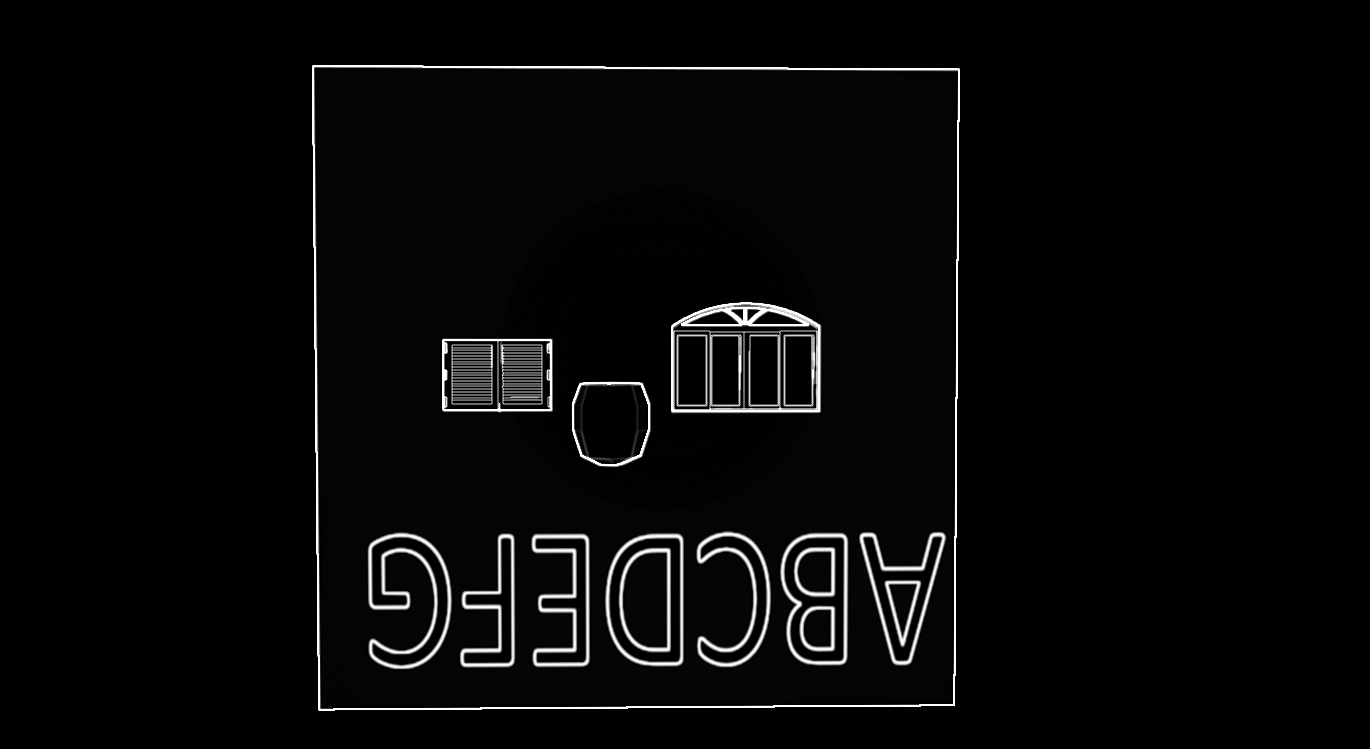
\includegraphics[scale=0.2]{images/aliased_value_example_3_temporal.png}
	\caption{Imagen hecha de los valores de \textit{aliasing} de cada píxel.}\label{fig:aliasedval3}
\end{figure}

\subsection{Modificaciones del Filtro de Nitidez}
Con el Filtro de Nitidez actual, se crea un pico de color cuando el píxel central es brillante y los píxeles vecinos están oscuros, esto ocurre porque los colores oscuros son cercanos a cero y no son capaces de cancelar el aumento al píxel central, el cual se multiplica por $5$. Un ejemplo del peor caso posible es tener el píxel central con un color brillante y los píxeles del vecindario como negro puro, que se representan como cero. Por lo tanto, hemos normalizado el Filtro de Nitidez para evitar crear ese pico de color y trabajar mejor con píxeles brillantes con vecindarios oscuros. El filtro se cambió de \ref{eq:sharpen} a:
\begin{equation} \label{eq:new_sharpen}
\centering
\begin{bmatrix*}[c]
0 & -0.25 &  0 \\
-0.25  &  2 & -0.25  \\
0 & -0.25  &  0
\end{bmatrix*}
\end{equation}

La Ecuación \ref{eq:new_sharpen} muestra la nueva matriz de convolución del Filtro de Nitidez utilizada.


\chapter{Results}
In this chapter, we explain how we evaluated the improvements done to the Temporal Anti-Aliasing. We show the numerical and visual results obtained. Finally, we explain the results and their meaning compared to the previous implementation of TAA and other Anti-Aliasing solutions.
\section{Evaluation Methodology}
To evaluate the improvements achieved to the Temporal Anti-Aliasing technique we selected models and camera angles that place the technique under stress. Then, using the Testing Framework we developed, we proceed to render and save images of each of those models to compare how the technique behaves in comparison to the original TAA implementation and other Anti-Aliasing techniques to determine if the proposed techniques in this thesis provided images with better quality without incurring heavy memory usage or time consumption. Also, a special test was taken to measure if changing the Sharpen Filter was the sole mechanism providing an improvement.

The models used on the tests were:
\begin{itemize}
\item Pipe: A brown pipe with hard edges.
\item Window with Blinds: A blue window with closed blinds.
\item Arched Window: A blue window with an arch at the top.
\item Wall: A white wall with black text.
\item Sponza Atrium: exemplifies a general scene.
\item Sponza Atrium Flowers: exemplifies a cutout model.
\item Hairball: contains many fine details for its numerous fibers.
\end{itemize}

It is important to note that in Computer Graphics there are only common models used to test techniques, there is no standard per se. On this Master Thesis, we used two common models: the Sponza Atrium, which has many variations and it is commonly used to test many Computer Graphics techniques; and Hairball, which is sometimes used to test Ray and Path Tracing techniques. As well, an explanation why each model was selected is available under each test subsection.

Note that Sponza Atrium and Hairball models were downloaded from Morgan McGuire's Computer Graphics Archive \cite{McGuire2017Data}; the Pipe model is from Spencer Arts \cite{Spencer2010}; the Arched Window model is from Isabela H. \cite{Isabela2016}; and the Window with Blinds is from Channa Yim \cite{Channa2015}.

The tests were performed on the computer provided by Lund University which has the following specification:
\begin{itemize}
\setlength\itemsep{0em}
\item CPU: Intel(R) Core(TM) i7-3820 CPU @ 3.60GHz, 3601 Mhz, 4 Cores, 8 Logical Processors
\item RAM: 64.0 GB	
\item GPU: NVIDIA GeForce GTX 1080 with 8 GB of VRAM
\item Rendering Resolution when not zooming: 1600 x 900
\end{itemize}

\section{Results and Comparisons}
First, we need to know that the best possible value for MSE and RMSD is zero, meaning that there is no error; that having a high PSNR and SNR value means it is better because the noise, which is the denominator in the equation of this metric, is close to zero; and, finally, that having an SSIM of $1$ means that the image is structurally the same as the ground truth, while having a value of $0$ means that it is structurally different. For the SSIM maps, each pixel represents its SSIM value; having a white color means that is structurally the same while having a darker color means that there are structural differences.

\subsection{Sharpen Filter}
For this test, we rendered the Sponza Atrium Model and a Static Sphere Model to evaluate the effects of the Normalized Sharpen Filter to the general quality of the rendered image, especially, regarding the blurring normally caused by TAA. Everything was rendered using both implementations of TAA with and without the Normalized Sharpen Filter to see if this change was the only improvement that was increasing the quality of the rendered image. The scene was selected for the test because it provided an example of a general scene that should not generate any blur. As we see from the Table \ref{tab:sharpen_res}, even if the Master Thesis TAA and the Uncharted TAA used the new Sharpen Filter, our other improvements still rendered a higher quality image. If we zoom on Figure \ref{fig:sharpen_render} From Figure \ref{fig:sharpen_ssim} we can see that the Normalized Sharpen Filter contributes reducing the artifacts in the rendered image, as there are almost no dark areas on the SSIM maps of the TAA's using it.

% Table generated by Excel2LaTeX from sheet 'Sharpen Filter'
\begin{table}[!hbt]
	\small
	\centering
	\caption{Sharpen Filter Test numerical results}
	\begin{tabular}{|m{2.5em}|c|c|c|c|c|}
		\hline
		\multicolumn{6}{|c|}{\textbf{Sharpen Filter Test}} \\
		\hline
		\textbf{\makecell{\diagbox[height=3em,innerwidth=2.5em]{Tests}{AA}}} & \textbf{\makecell{Uncharted \\ TAA \\ Not \\ Normalized}} & \textbf{\makecell{Uncharted \\ TAA \\ Normalized}} & \textbf{\makecell{Master \\ TAA \\ Not \\ Normalized}} & \textbf{\makecell{Master \\ TAA \\ Normalized}} & \textbf{\makecell{Best} } \\
		\hline
		MSE   & 149.271 & 8.835 & 148.036 & 8.224 & \textbf{\makecell{\scriptsize Master \\ \scriptsize TAA \\ \scriptsize Normalized}} \\
		\hline
		RMSD  & 12.218 & 2.972 & 12.167 & 2.868 & \textbf{\makecell{\scriptsize Master \\ \scriptsize TAA \\ \scriptsize Normalized}} \\
		\hline
		Peak-SNR  & 26.391 & 38.669 & 26.427 & 38.980 & \textbf{\makecell{\scriptsize Master \\ \scriptsize TAA \\ \scriptsize Normalized}} \\
		\hline
		SNR   & 16.245 & 28.522 & 16.281 & 28.833 & \textbf{\makecell{\scriptsize Master \\ \scriptsize TAA \\ \scriptsize Normalized}} \\
		\hline
		SSIM  & 0.932 & 0.992 & 0.933 & 0.992 & \textbf{\makecell{\scriptsize Master \\ \scriptsize TAA \\ \scriptsize Normalized}} \\
		\hline
	\end{tabular}%
	\label{tab:sharpen_res}%
\end{table}%

\begin{figure}[H]
	\centering
	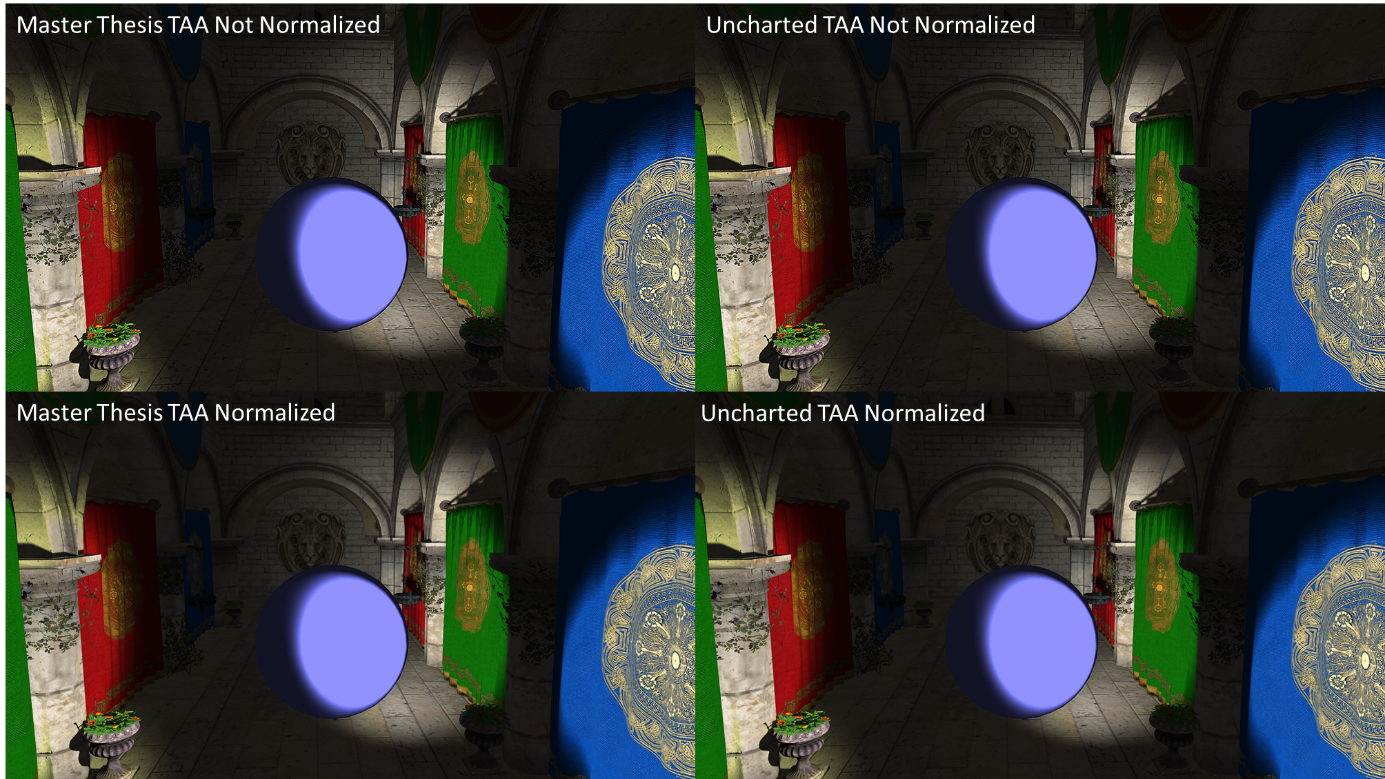
\includegraphics[scale=0.9]{images/results/sharpen_test_render.png}
	\caption{Rendered Images comparison.}\label{fig:sharpen_render}
\end{figure}

\begin{figure}[H]
	\centering
	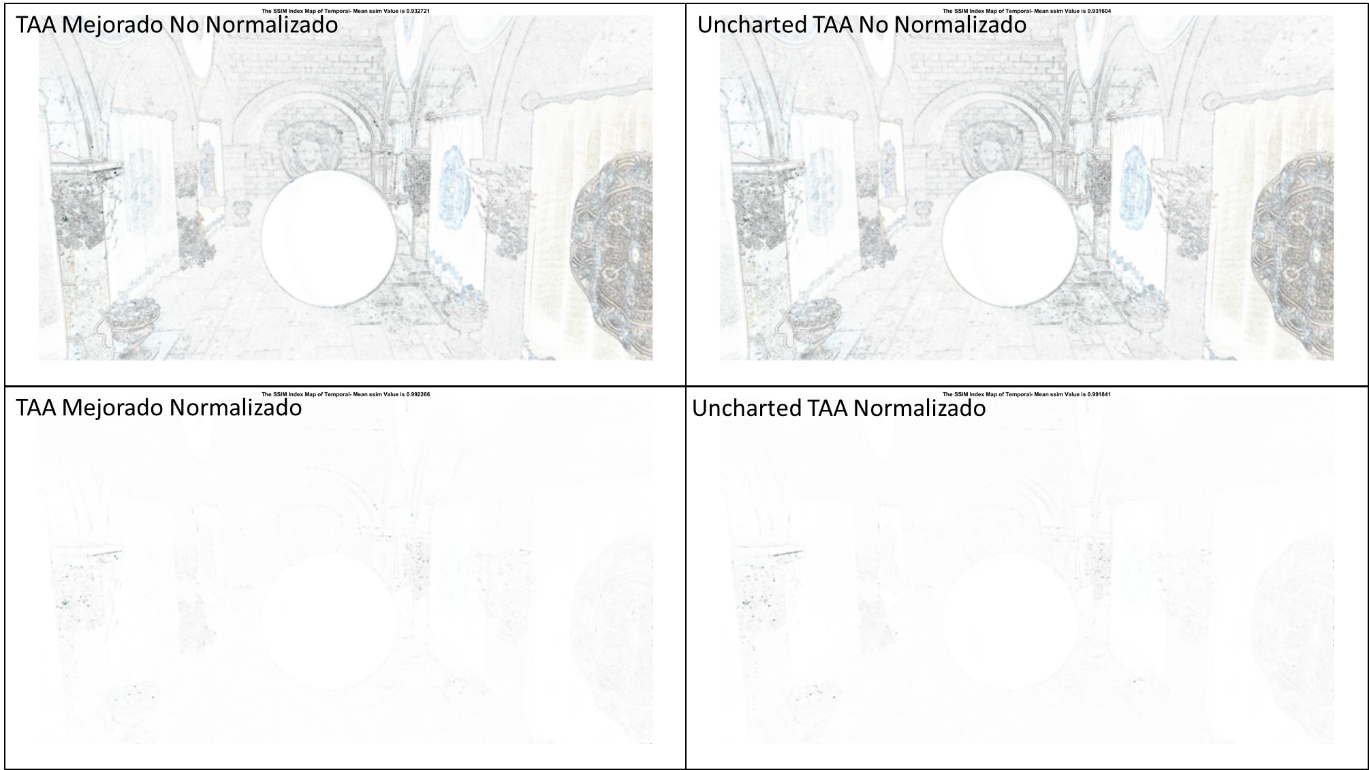
\includegraphics[scale=0.9]{images/results/sharpen_test_ssim.png}
	\caption{SSIM Maps comparison.}\label{fig:sharpen_ssim}
\end{figure}

\subsection{Pipe}
For this test, we rendered the Pipe Model in order to test how the improvements behaved when rendering a model with hard edges. We wanted to test if our improvements reduced the amount of blur around those hard edges while still fixing the aliasing problem. We rendered the Pipe twice, the first time using a regular camera angle, for normal aliasing around the edges, and a skewed camera angle, for increased aliasing effects. As we see from the results, TAA with our improvements is at the same quality level as SMAA. 

\subsubsection{Regular}
When we zoom and compare Figure \ref{fig:pipe_regular_truth} with the rendered images in Figure \ref{fig:pipe_regular_render}, especially around the edges, we observe that there is a reduction of blurring in the Master Thesis TAA in comparison with the Uncharted TAA. As well, we observe that the Uncharted TAA generates bright colors around the edges which should not be there; this is easier to observe as the dark edges on the SSIM map of the Uncharted TAA on Figure \ref{fig:pipe_regular_render}. Furthermore, Table \ref{tab:pipe_regular} confirm us that the Master Thesis TAA reaches almost the same quality as SMAA.

% Table generated by Excel2LaTeX from sheet 'Pipe Regular'
\begin{table}[!hbt]	
	\small
	\centering
	\caption{Numerical results of the Pipe Test with regular camera inclination.}
	\begin{tabular}{|l|c|c|c|c|c|c|c|}
		\hline
		\multicolumn{8}{|c|}{\textbf{Pipe Regular Test}} \\
		\hline
		\textbf{\diagbox{Tests}{AA}} & \textbf{No AA} & \textbf{FXAA}  & \textbf{SMAA}  & \textbf{\makecell{Uncharted \\ TAA}} & \textbf{\makecell{Master \\ TAA}} & \textbf{Best} & \textbf{\makecell{Master \\ TAA \\ Against \\ Best}} \\
		\hline
		MSE   & 8.608 & 3.573 & 1.278 & 14.602 & 1.574 & SMAA  & -0.296 \\
		\hline
		RMSD  & 2.934 & 1.890 & 1.130 & 3.821 & 1.254 & SMAA  & -0.124 \\
		\hline
		Peak-SNR  & 38.782 & 42.601 & 47.066 & 36.487 & 46.162 & SMAA  & 0.904 \\
		\hline
		SNR   & 36.451 & 40.270 & 44.735 & 34.156 & 43.831 & SMAA  & 0.904 \\
		\hline
		SSIM  & 0.999 & 0.999 & 1.000 & 0.996 & 1.000 & SMAA  & 0.000 \\
		\hline
	\end{tabular}%
	\label{tab:pipe_regular}%
\end{table}%

\begin{figure}[H]
	\centering
	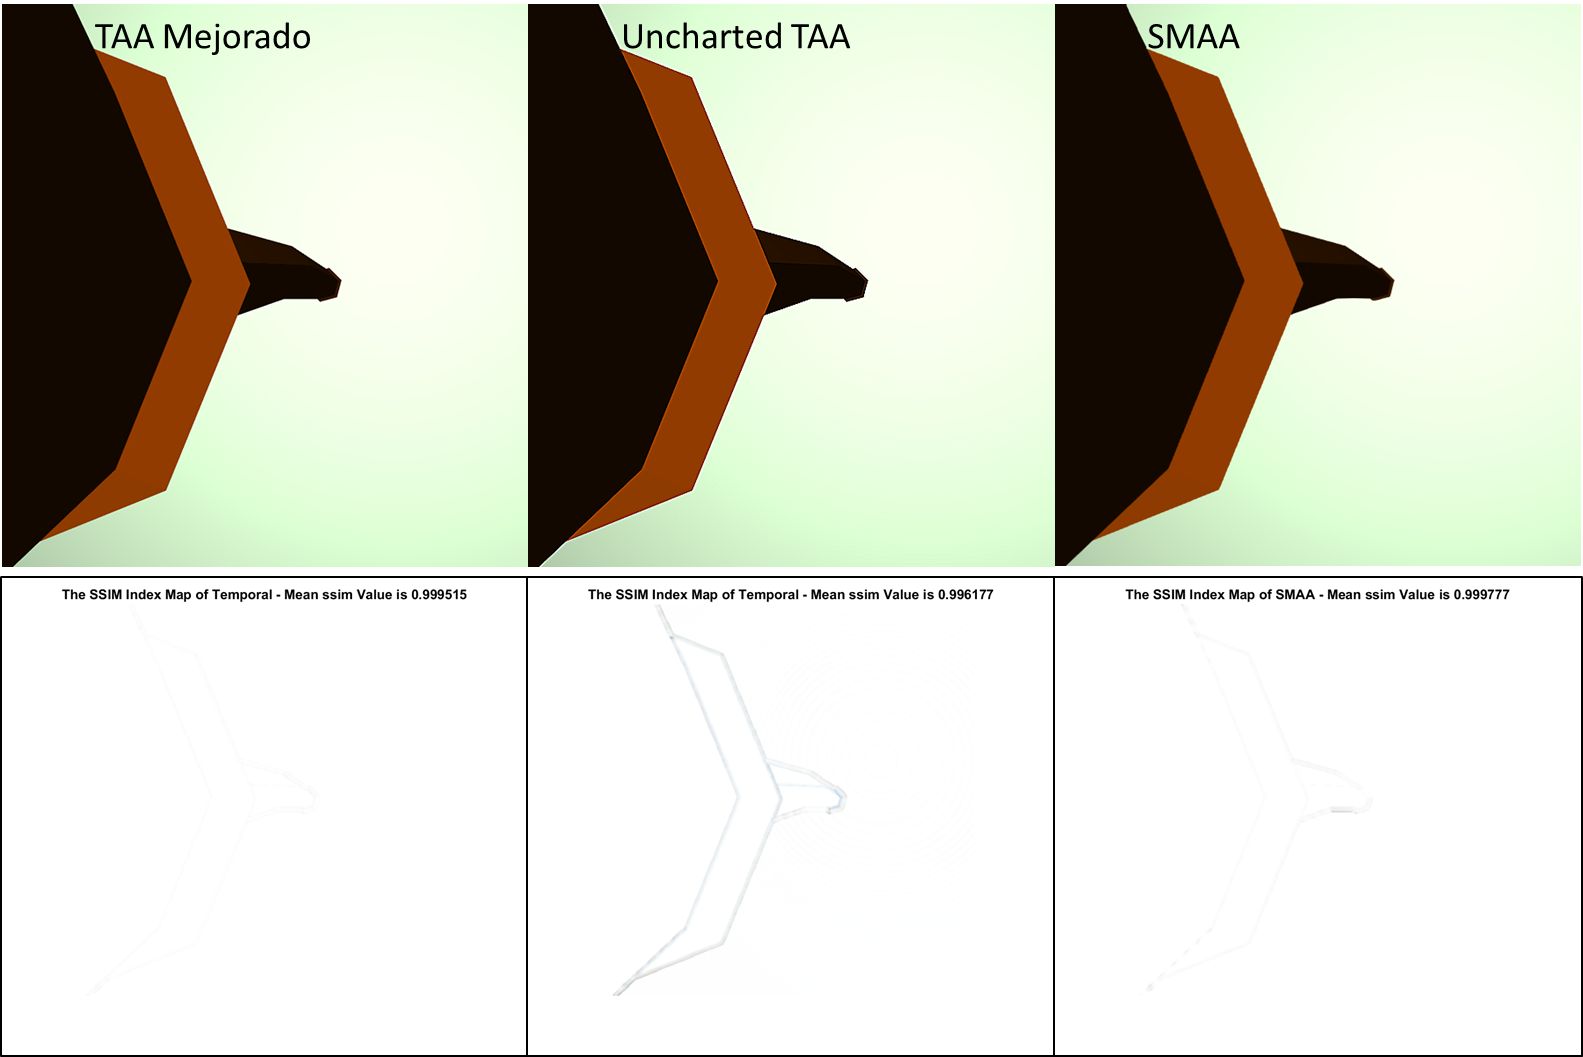
\includegraphics[scale=0.5]{images/results/pipe_regular.png}
	\caption{Pipe Regular comparison between Master Thesis TAA, Uncharted TAA, and SMAA.}\label{fig:pipe_regular_render}
\end{figure}

\begin{figure}[H]
	\centering
	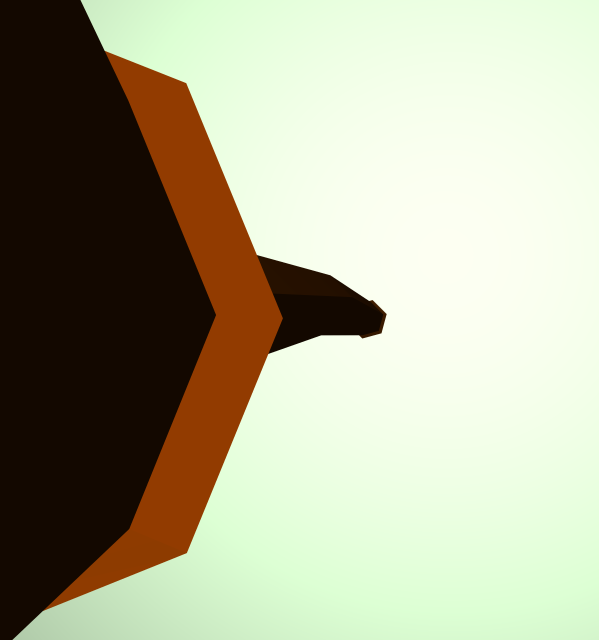
\includegraphics[scale=0.2]{images/results/pipe_regular_sobel_ground_truth.png}
	\caption{Pipe Regular Test ground truth.}\label{fig:pipe_regular_truth}
\end{figure}


\subsubsection{With Camera Inclination}
Zooming and comparing the Figures \ref{fig:pipe_inclination_render} and \ref{fig:pipe_inclination_truth}, we can observe that the Master TAA is the most similar to the Ground Truth. From the SSIM map of the Uncharted TAA, we notice that blurring is being generated around the edges. 

Finally, from Figure \ref{fig:pipe_inclination_render} and Table \ref{fig:pipe_inclination_truth} we note that SMAA is not properly detecting the upper edge of the pipe, when zoomed we observe a small staircase forming around the edge.  This is due to the fact that the camera was set up with a skewed inclination which pushed to the limit the edge detection techniques used in SMAA.

% Table generated by Excel2LaTeX from sheet 'Pipe with Inclination'
\begin{table}[H]
	\small
	\centering
	\caption{Numerical results of the Pipe Test with a skewed camera inclination.}
	\begin{tabular}{|l|c|c|c|c|c|c|c|}
		\hline
		\multicolumn{8}{|c|}{\textbf{Pipe with Camera Inclination Test}} \\
		\hline
		\textbf{\diagbox{Tests}{AA}} & \textbf{No AA} & \textbf{FXAA}  & \textbf{SMAA}  & \textbf{\makecell{Uncharted \\ TAA}} & \textbf{\makecell{Master \\ TAA}} & \textbf{Best} & \textbf{\makecell{Master \\ TAA \\ Against \\ Best}} \\
		\hline
		MSE   & 16.112 & 6.470 & 2.810 & 14.349 & 2.664 & Master TAA & 0.000 \\
		\hline
		RMSD  & 4.014 & 2.544 & 1.676 & 3.788 & 1.632 & Master TAA & 0.000 \\
		\hline
		Peak-SNR  & 36.059 & 40.022 & 43.644 & 36.563 & 43.876 & Master TAA & 0.000 \\
		\hline
		SNR   & 32.474 & 36.437 & 40.059 & 32.978 & 40.291 & Master TAA & 0.000 \\
		\hline
		SSIM  & 0.998 & 0.999 & 1.000 & 0.996 & 0.999 & SMAA  & 0.000 \\
		\hline
	\end{tabular}%
	\label{tab:pipe_inclination}%
\end{table}%

\begin{figure}[H]
	\centering
	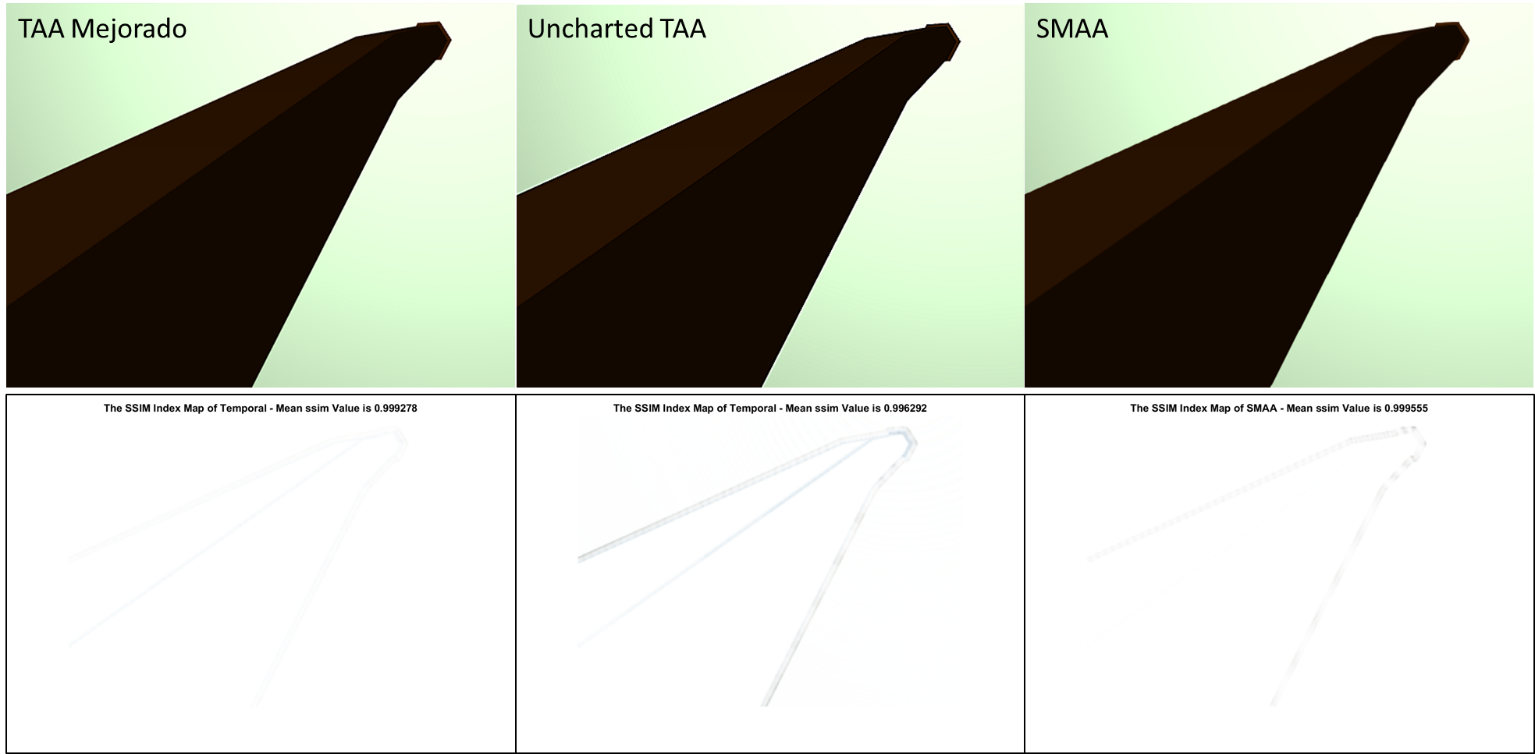
\includegraphics[scale=0.7]{images/results/pipe_inclination.png}
	\caption{Pipe with Camera Inclination comparison between Master Thesis TAA, Uncharted TAA, and SMAA.}\label{fig:pipe_inclination_render}
\end{figure}

\begin{figure}[H]
	\centering
	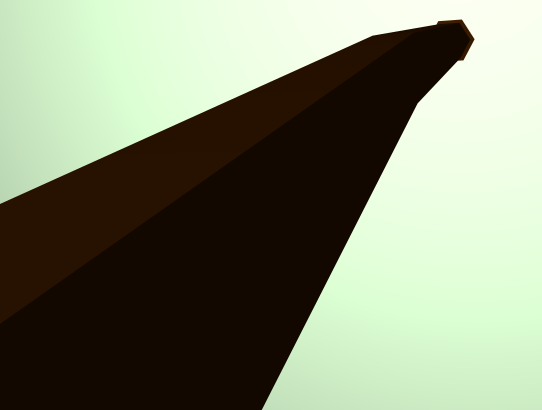
\includegraphics[scale=0.2]{images/results/pipe_with_inclination_sobel_ground_truth.png}
	\caption{Pipe with Camera Inclination Test ground truth.}\label{fig:pipe_inclination_truth}
\end{figure}


\subsection{Window with Blinds}
On this test, we used the Window with Blinds model for its small details at the blinds. We tested how our improvements behaved with this kind of details and discovered that it did not react in a proper way even if the numerical results showed otherwise.

From Figures \ref{fig:window_blind_render} and \ref{fig:window_blind_truth} we can observe it is complicated for the techniques to handle the small gaps between the blinds. From Figure \ref{fig:window_blind_render} and Table \ref{tab:window_blind}, we notice that the Master Thesis TAA and SMAA are able to reconstruct more details than the Uncharted TAA but, aesthetically and visually, we believe it is better the Uncharted TAA than the other techniques because those small gaps between the blinds flicker less when moving.

% Table generated by Excel2LaTeX from sheet 'Window Blind'
\begin{table}[H]
	\small
	\centering
	\caption{Numerical results of the Window with Blinds Test.}
	\begin{tabular}{|l|c|c|c|c|c|c|c|}
		\hline
		\multicolumn{8}{|c|}{\textbf{Window with Blinds Test}} \\
		\hline
		\textbf{\diagbox{Tests}{AA}} & \textbf{No AA} & \textbf{FXAA}  & \textbf{SMAA}  & \textbf{\makecell{Uncharted \\ TAA}} & \textbf{\makecell{Master \\ TAA}} & \textbf{Best} & \textbf{\makecell{Master \\ TAA \\ Against \\ Best}} \\
		\hline
		MSE   & 96.044 & 70.486 & 35.134 & 170.229 & 32.115 & Master TAA & 0.000 \\
		\hline
		RMSD  & 9.800 & 8.396 & 5.927 & 13.047 & 5.667 & Master TAA & 0.000 \\
		\hline
		Peak-SNR  & 28.306 & 29.650 & 32.674 & 25.820 & 33.064 & Master TAA & 0.000 \\
		\hline
		SNR   & 25.467 & 26.810 & 29.834 & 22.981 & 30.224 & Master TAA & 0.000 \\
		\hline
		SSIM  & 0.986 & 0.990 & 0.995 & 0.976 & 0.995 & Master TAA  & 0.000 \\
		\hline
	\end{tabular}%
	\label{tab:window_blind}%
\end{table}%

\begin{figure}[H]
	\centering
	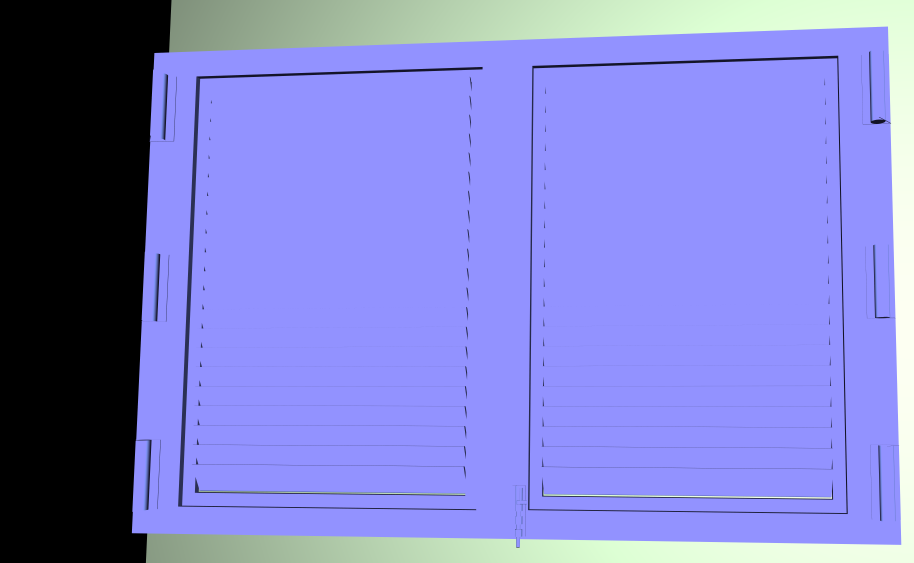
\includegraphics[scale=0.14]{images/results/window_blind_sobel_ground_truth.png}
	\caption{Window with Blinds ground truth.}\label{fig:window_blind_truth}
\end{figure}

\begin{figure}[H]
	\centering
	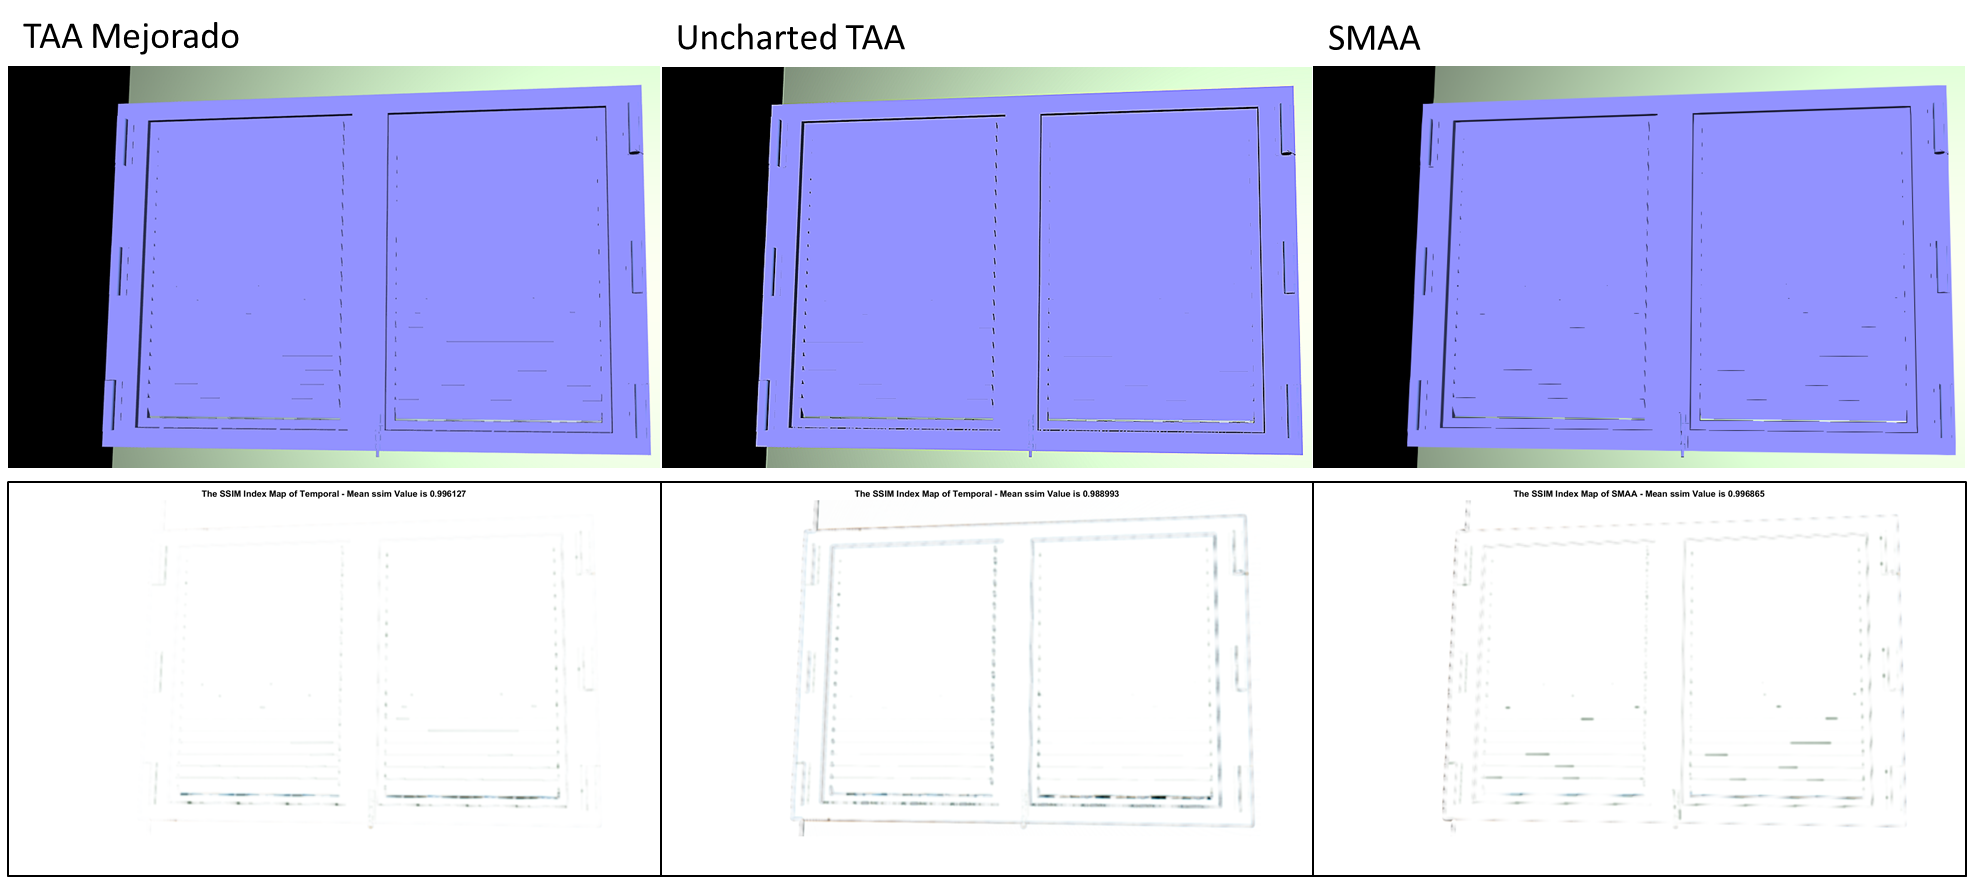
\includegraphics[scale=0.8]{images/results/window_blind.png}
	\caption{Window with Blinds comparison between Master Thesis TAA, Uncharted TAA, and SMAA.}\label{fig:window_blind_render}
\end{figure}



\subsection{Arched Window}
We used the Arched Window Model to test how our improved implementation with the small details of the window’s door and the aliasing from the arch. We can observe from Figures \ref{fig:window_arch_render} and \ref{fig:window_arch_truth} that for all the techniques, the small gaps around the window's door are hard to render. On some parts small gaps, we see that the techniques could not render it completely. Even though on Table \ref{tab:window_arch} SMAA appears to be the best, but we believe that the Uncharted TAA has the best visual quality because those incomplete gaps generate flickering when there is movement.
% Table generated by Excel2LaTeX from sheet 'Arched Window'
\begin{table}[H]
	\small
	\centering
	\caption{Numerical results of the Arched Window Test.}
	\begin{tabular}{|l|c|c|c|c|c|c|c|}
		\hline
		\multicolumn{8}{|c|}{\textbf{Arched Window Test}} \\
		\hline
		\textbf{\diagbox{Tests}{AA}} & \textbf{No AA} & \textbf{FXAA}  & \textbf{SMAA}  & \textbf{\makecell{Uncharted \\ TAA}} & \textbf{\makecell{Master \\ TAA}} & \textbf{Best} & \textbf{\makecell{Master \\ TAA \\ Against \\ Best}} \\
		\hline
		MSE   & 56.313 & 39.103 & 19.849 & 76.483 & 21.983 & SMAA  & -2.134 \\
		\hline
		RMSD  & 7.504 & 6.253 & 4.455 & 8.745 & 4.689 & SMAA  & -0.233 \\
		\hline
		Peak-SNR  & 30.625 & 32.209 & 35.153 & 29.295 & 34.710 & SMAA  & 0.443 \\
		\hline
		SNR   & 27.325 & 28.909 & 31.854 & 25.996 & 31.410 & SMAA  & 0.443 \\
		\hline
		SSIM  & 0.992 & 0.994 & 0.997 & 0.989 & 0.996 & SMAA  & 0.001 \\
		\hline
	\end{tabular}%
	\label{tab:window_arch}%
\end{table}%

\begin{figure}[H]
	\centering
	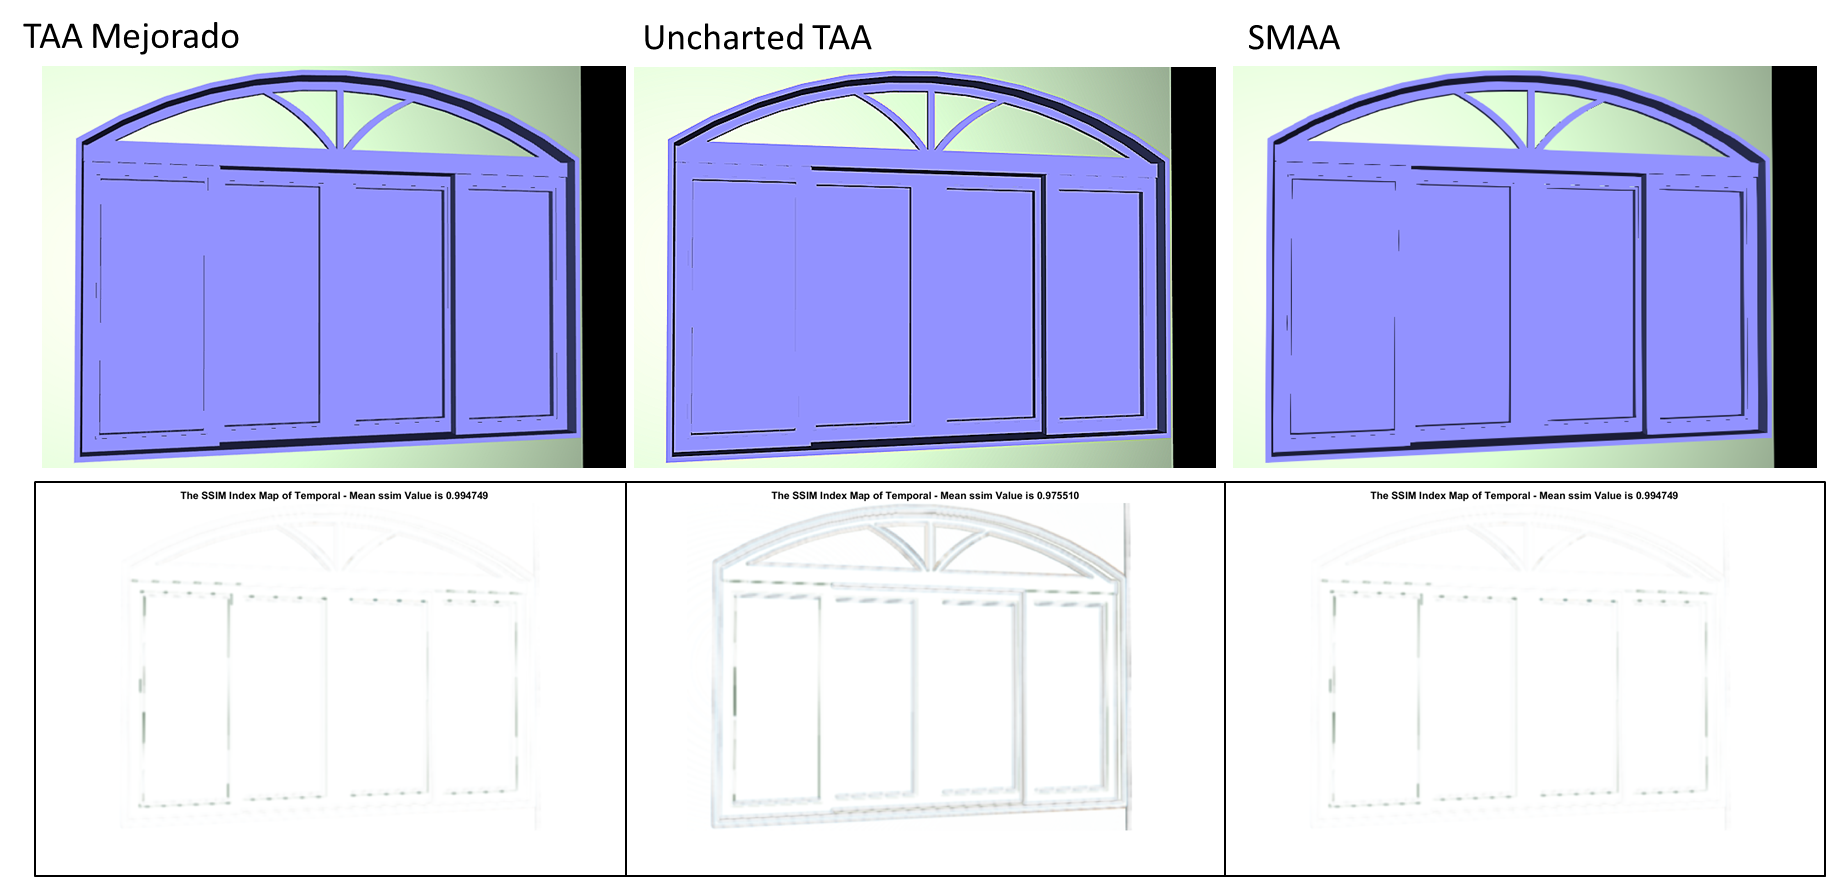
\includegraphics[scale=0.8]{images/results/window_arch.png}
	\caption{Arched Window comparison between Master Thesis TAA, Uncharted TAA, and SMAA.}\label{fig:window_arch_render}
\end{figure}

\begin{figure}[H]
	\centering
	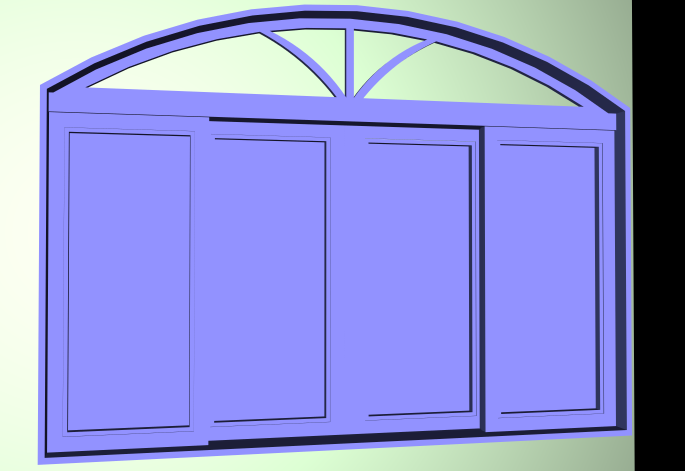
\includegraphics[scale=0.18]{images/results/window_arch_sobel_ground_truth.png}
	\caption{Arched Window ground truth.}\label{fig:window_arch_truth}
\end{figure}

\subsection{Sponza Atrium}
For this test, we wanted to analyze how the Master TAA implementation behaved with a general scene with lights and shadows, we used the Sponza Atrium Model with the Sphere Model being static in the center.

If we compare Figures \ref{fig:sponza_render} and \ref{fig:sponza_truth}, we can observe that the Uncharted TAA had blurring problems around all the edges, which is visible on its SSIM map; SMAA had problems with all the flowers, we can observe the flower shape on its SSIM map; and that the Master Thesis TAA only had minor problems with the flowers, as seen on the gray areas on its SSIM map. Furthermore, Table \ref{tab:sponza} confirm what we are observing on the visual results, as the Master Thesis TAA got the best scores on most of the test; the Uncharted TAA got the worst scores due to the edges problems; and SMAA got worse than normally scores due to the flowers problem.
% Table generated by Excel2LaTeX from sheet 'Sponza Table'
\begin{table}[H]
	\small
	\centering
	\caption{Numerical results of the Sponza Atrium Test.}
	\begin{tabular}{|l|c|c|c|c|c|c|c|}
		\hline
		\multicolumn{8}{|c|}{\textbf{Sponza Atrium Test}} \\
		\hline
		\textbf{\diagbox{Tests}{AA}} & \textbf{No AA} & \textbf{FXAA}  & \textbf{SMAA}  & \textbf{\makecell{Uncharted \\ TAA}} & \textbf{\makecell{Master \\ TAA}} & \textbf{Best} & \textbf{\makecell{Master \\ TAA \\ Against \\ Best}} \\
		\hline
		MSE   & 13.458 & 8.290 & 8.610 & 42.728 & 3.972 & Master TAA & 0.000 \\
		\hline
		RMSD  & 3.669 & 2.879 & 2.934 & 6.537 & 1.993 & Master TAA & 0.000 \\
		\hline
		Peak-SNR  & 36.841 & 38.945 & 38.781 & 31.824 & 42.141 & Master TAA & 0.000 \\
		\hline
		SNR   & 20.056 & 22.160 & 21.996 & 15.038 & 25.356 & Master TAA & 0.000 \\
		\hline
		SSIM  & 0.988 & 0.991 & 0.991 & 0.938 & 0.991 & Master TAA  & 0.000 \\
		\hline
	\end{tabular}%
	\label{tab:sponza}%
\end{table}%

\begin{figure}[H]
	\centering
	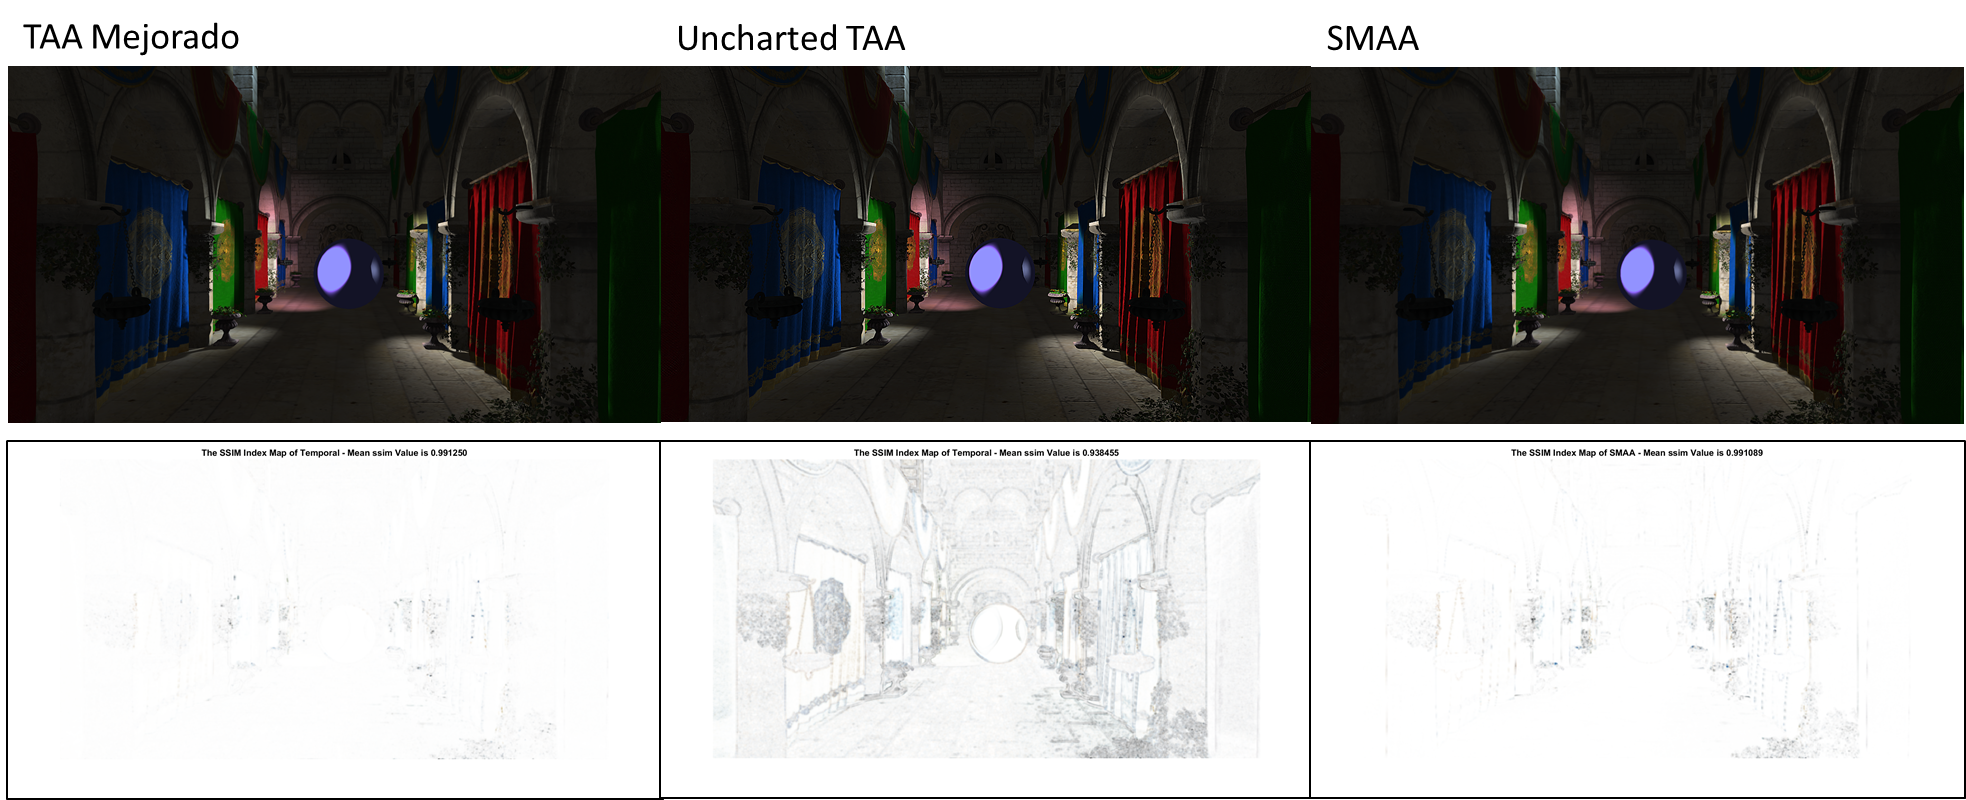
\includegraphics[scale=0.9]{images/results/sponza.png}
	\caption{Sponza Atrium comparison between Master Thesis TAA, Uncharted TAA, and SMAA.}\label{fig:sponza_render}
\end{figure}

\begin{figure}[H]
	\centering
	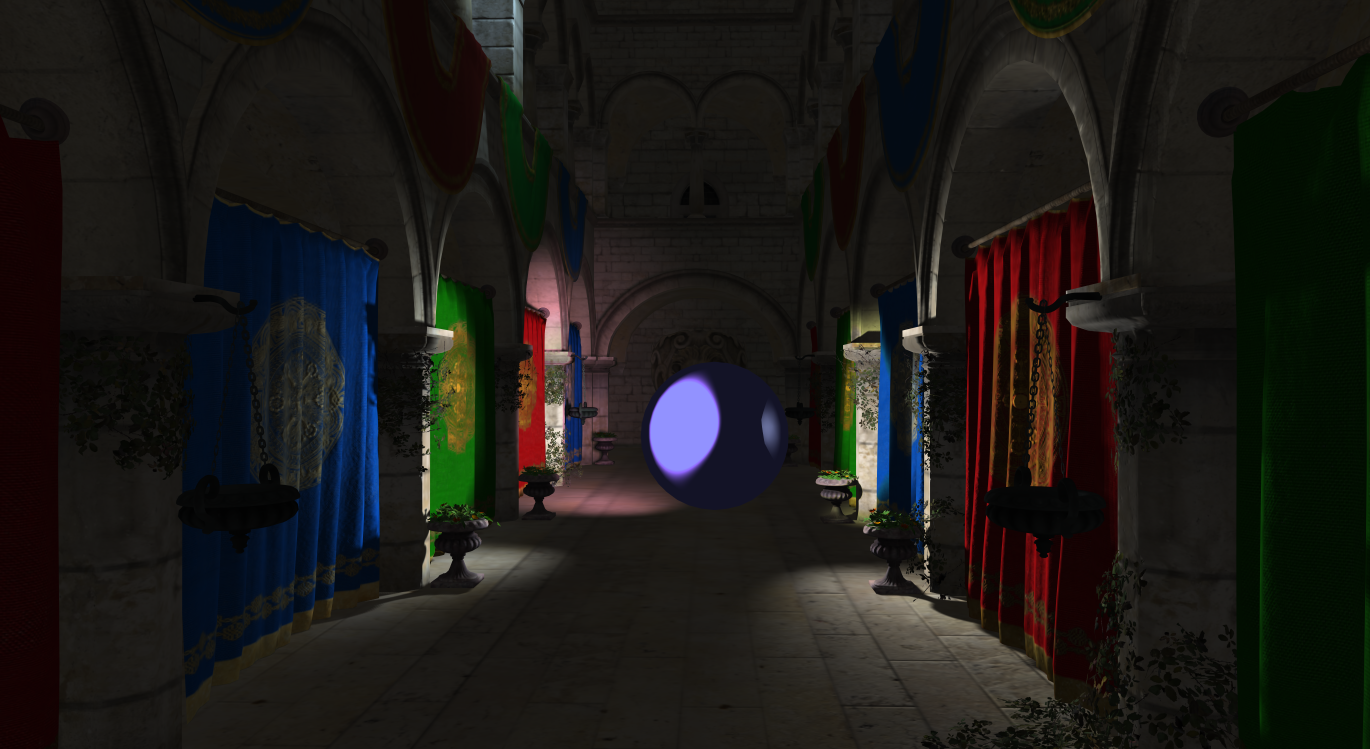
\includegraphics[scale=0.1]{images/results/sponza_sobel_ground_truth.png}
	\caption{Sponza Atrium ground truth.}\label{fig:sponza_truth}
\end{figure}

\subsection{Sponza Atrium Flowers}
On this test, we looked at how do our improvements handle the details of a model with transparent parts, as in the Flowers from the Sponza Atrium Model, because the aliasing they present is considered hard to properly detect and correct.

From Figures \ref{fig:sponza_flowers_render} and \ref{fig:sponza_flowers_truth}, we observe the Uncharted TAA has many problems handling this type of model, especially if we look at its SSIM map; we notice that SMAA could not correct all the aliasing artifacts from the edges of the flowers, we see the edges of the flowers appear on its SSIM map; and, finally, we observe that the Master Thesis TAA corrected the most aliasing artifacts, some are still left as seen on its SSIM map on the gray areas. Furthermore, Table \ref{tab:sponza_flowers} confirm what we observe visually, as the Master TAA got the best scores and SMAA scored worse than average.

% Table generated by Excel2LaTeX from sheet 'Sponza Flowers'
\begin{table}[H]
	\small
	\centering
	\caption{Numerical results of the Sponza Atrium Flowers Test.}
	\begin{tabular}{|l|c|c|c|c|c|c|c|}
		\hline
		\multicolumn{8}{|c|}{\textbf{Sponza Atrium Flowers Test}} \\
		\hline
		\textbf{\diagbox{Tests}{AA}} & \textbf{No AA} & \textbf{FXAA}  & \textbf{SMAA}  & \textbf{\makecell{Uncharted \\ TAA}} & \textbf{\makecell{Master \\ TAA}} & \textbf{Best} & \textbf{\makecell{Master \\ TAA \\ Against \\ Best}} \\
		\hline
		MSE   & 122.795 & 66.062 & 72.279 & 490.281 & 36.162 & Master TAA & 0.000 \\
		\hline
		RMSD  & 11.081 & 8.128 & 8.502 & 22.142 & 6.013 & Master TAA & 0.000 \\
		\hline
		Peak-SNR  & 27.239 & 29.931 & 29.541 & 21.226 & 32.548 & Master TAA & 0.000 \\
		\hline
		SNR   & 19.590 & 22.282 & 21.891 & 13.577 & 24.899 & Master TAA & 0.000 \\
		\hline
		SSIM  & 0.959 & 0.975 & 0.972 & 0.863 & 0.985 & Master TAA & 0.000 \\
		\hline
	\end{tabular}%
	\label{tab:sponza_flowers}%
\end{table}%

\begin{figure}[H]
	\centering
	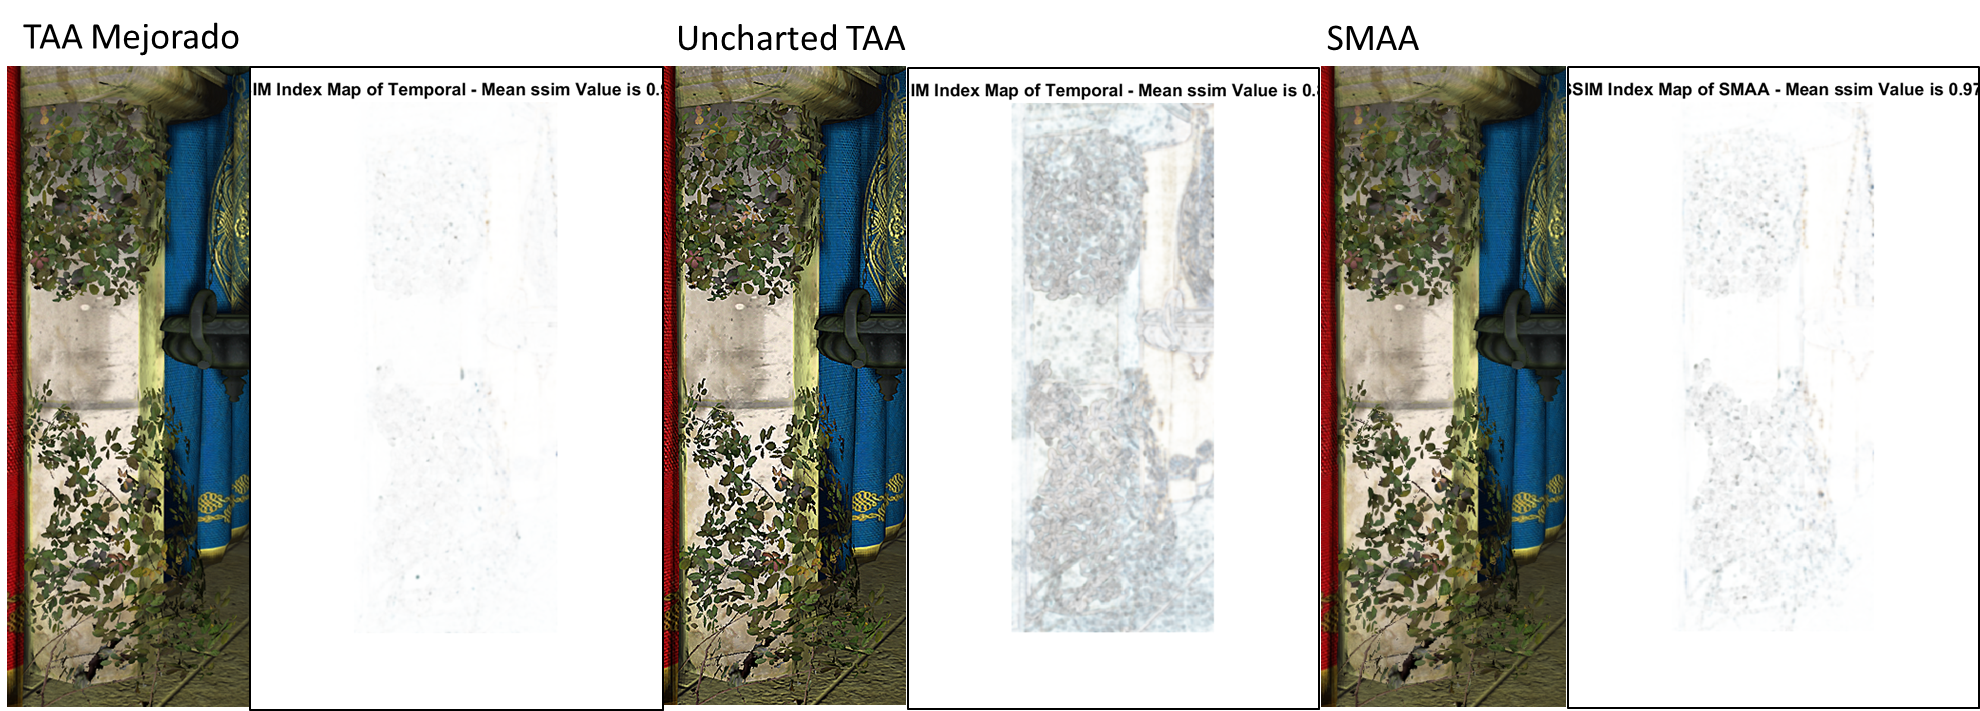
\includegraphics[scale=0.9]{images/results/sponza_flowers.png}
	\caption{Sponza Atrium Flowers comparison between Master Thesis TAA, Uncharted TAA, and SMAA.}\label{fig:sponza_flowers_render}
\end{figure}

\begin{figure}[H]
	\centering
	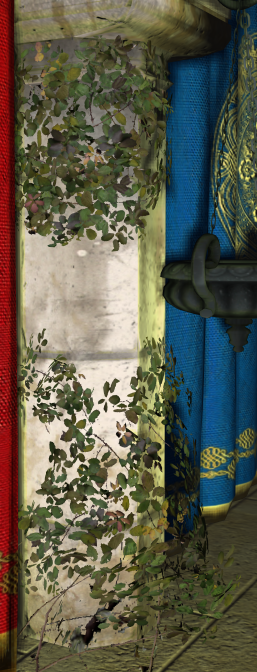
\includegraphics[scale=0.2]{images/results/sponza_flowers_sobel_ground_truth.png}
	\caption{Sponza Atrium Flowers ground truth.}\label{fig:sponza_flowers_truth}
\end{figure}

\subsection{Hard Edges}
For this test, we explored how the Master Thesis Implementation with many small details at a far distance and how it behaved with hard edges. We used both Windows Models for the small details and the Pipe and Wall Models for the hard edges. 

From Figures \ref{fig:hard_test_render} and \ref{fig:hard_test_truth}, we observe that the Master TAA is the best technique for handling all the edges from all the models, its SSIM map barely has any dark area and on Table \ref{tab:hard_test} it surpasses any other technique; the Uncharted TAA creates blurring around all the edges, this appears on its SSIM maps as all the edges are visible; and SMAA fail to correct some aliasing artifacts which we can observe on its SSIM map.

% Table generated by Excel2LaTeX from sheet 'Hard Test'
\begin{table}[H]
	\small
	\centering
	\caption{Numerical results of the Hard Edges Test.}
	\begin{tabular}{|l|c|c|c|c|c|c|c|}
		\hline
		\multicolumn{8}{|c|}{\textbf{Hard Edges Test}} \\
		\hline
		\textbf{\diagbox{Tests}{AA}} & \textbf{No AA} & \textbf{FXAA}  & \textbf{SMAA}  & \textbf{\makecell{Uncharted \\ TAA}} & \textbf{\makecell{Master \\ TAA}} & \textbf{Best} & \textbf{\makecell{Master \\ TAA \\ Against \\ Best}} \\
		\hline
		MSE   & 12.463 & 9.342 & 8.019 & 31.385 & 5.012 & Master TAA & 0.000 \\
		\hline
		RMSD  & 3.530 & 3.057 & 2.832 & 5.602 & 2.239 & Master TAA & 0.000 \\
		\hline
		Peak-SNR  & 37.174 & 38.426 & 39.090 & 33.164 & 41.131 & Master TAA & 0.000 \\
		\hline
		SNR   & 30.327 & 31.579 & 32.242 & 26.316 & 34.283 & Master TAA & 0.000 \\
		\hline
		SSIM  & 0.997 & 0.997 & 0.998 & 0.989 & 0.998 & Master TAA & 0.000 \\
		\hline
	\end{tabular}%
	\label{tab:hard_test}%
\end{table}%


\begin{figure}[H]
	\centering
	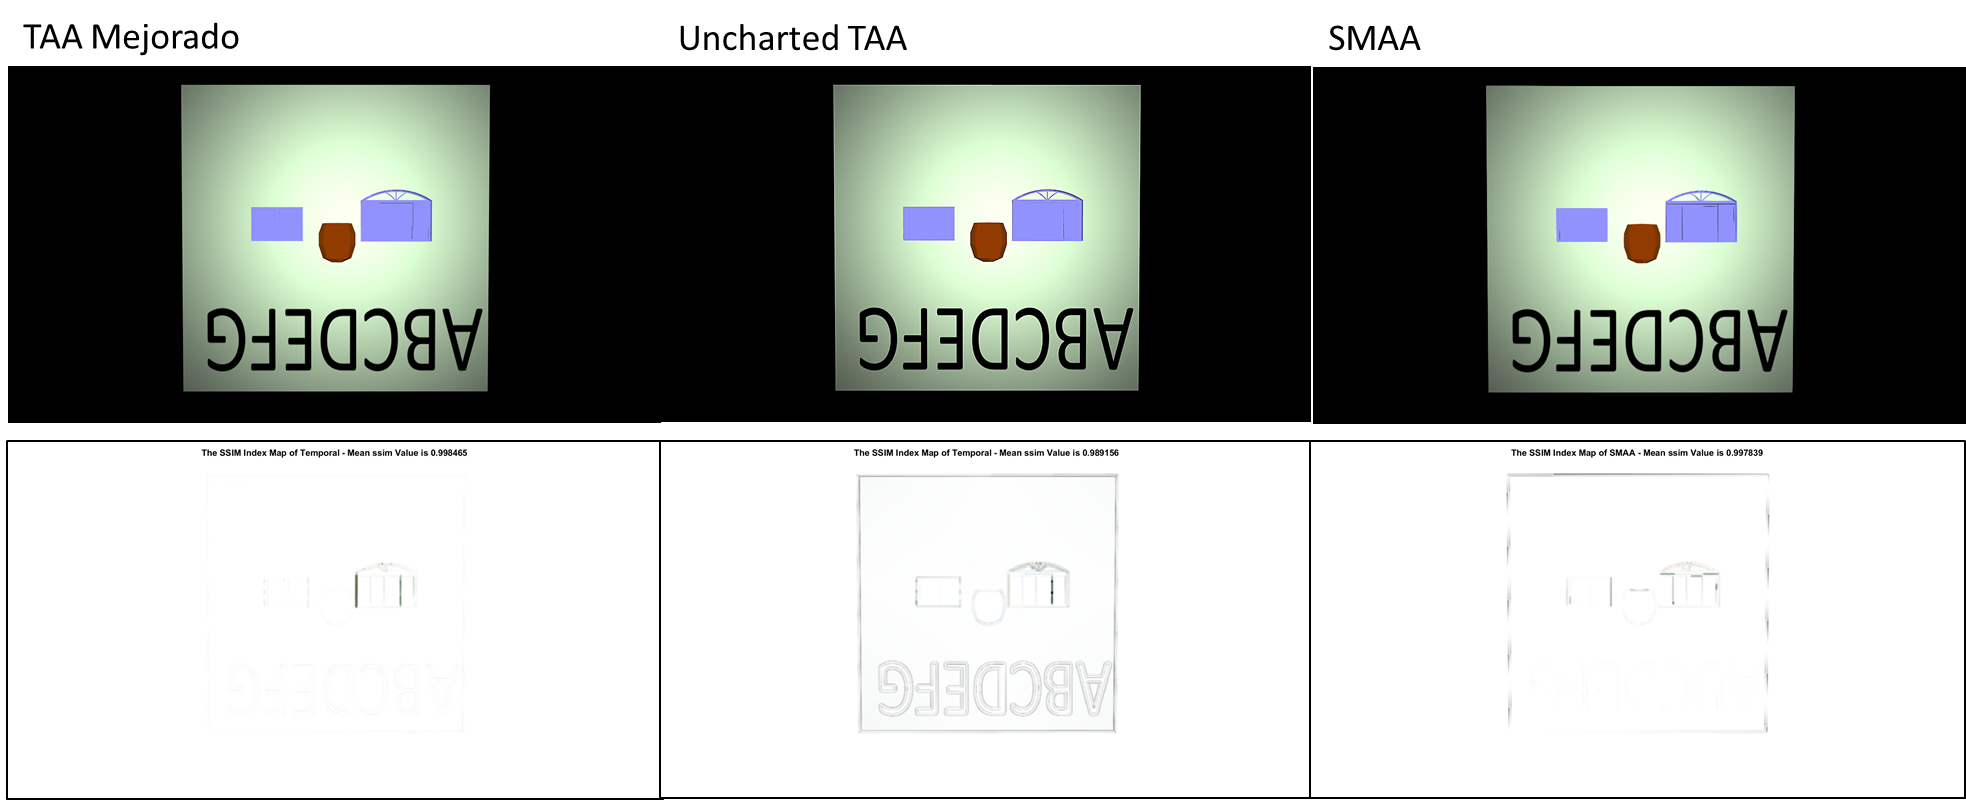
\includegraphics[scale=0.9]{images/results/hard_test.png}
	\caption{Hard Edges comparison between Master Thesis TAA, Uncharted TAA, and SMAA.}\label{fig:hard_test_render}
\end{figure}

\begin{figure}[H]
	\centering
	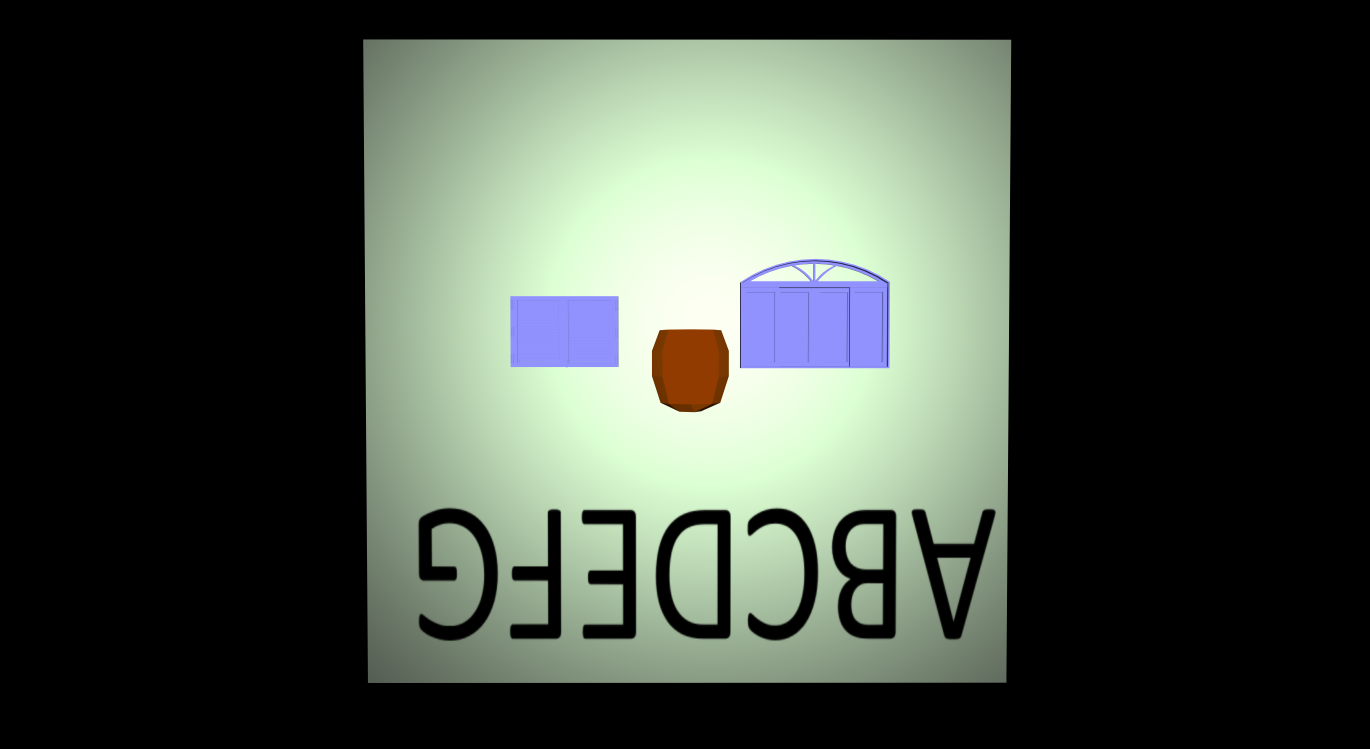
\includegraphics[scale=0.09]{images/results/hard_test_sobel_ground_truth.png}
	\caption{Hard Edges ground truth.}\label{fig:hard_test_truth}
\end{figure}


\subsection{Sphere Ghosting}
For this test, we wanted to measure how the improvements we performed decreased the effects of ghosting that were present in the Uncharted Implementation. For this reason, we selected the Sphere Model to move in the hall of the Sponza Atrium and rendered it under a camera angle that showed us ghosting trails. 

As we see from the visual results on Figure \ref{fig:sphere_ghosting}, ghosting effects were diminished in our implementation as the stripes visible on the Uncharted TAA are almost invisible on the Master Thesis TAA. Furthermore, in Table \ref{tab:sphere_ghosting} the average results on the Master TAA image metrics are better than the average from the Uncharted TAA. 

It is important to note that some metrics got an infinite result as they were exactly the same as the ground truth. This happens on some images in which the spheres cover the whole frame with a dark blue color. As well, the Test Index marks which test the associated result belongs to; on the averages we use Not Applicable (N\\A) because those results come from the average of all the tests. 
% Table generated by Excel2LaTeX from sheet 'Sphere Ghosting'
\begin{table}[H]
	\small
	\centering
	\caption{Numerical results summary of the 100 tests performed for the Sphere Ghosting Test.}
	\begin{tabular}{|l|c|c|c|c|}
		\hline
		\multicolumn{5}{|c|}{\textbf{Sphere Ghosting Test Summary}} \\
		\hline
		\multicolumn{1}{|c|}{\textbf{\diagbox{Tests}{AA}}} & \textbf{Uncharted TAA} & \textbf{Test Index} & \textbf{Master TAA} & \textbf{Test Index} \\
		\hline
		Best MSE & 0.000 & 63 & 0.000 & 63 \\
		\hline
		Worst MSE & 100.871 & 19 & 91.766 & 29 \\
		\hline
		Average MSE & 28.634 & N/A   & 19.501 & N/A \\
		\hline
		Best Peak-SNR & Inf   & 63 & Inf   & 63 \\
		\hline
		Worst Peak-SNR & 28.093 & 19 & 28.504 & 29 \\
		\hline
		Average Peak-SNR  & Inf   & N/A   & Inf   & N/A \\
		\hline
		Best SNR & Inf   & 63 & Inf   & 63 \\
		\hline
		Worst SNR & 16.818 & 11 & 18.524 & 29 \\
		\hline
		Average SNR  & Inf   & N/A   & Inf   & N/A \\
		\hline
		Best SSIM & 1.000 & 63 & 1.000 & 63 \\
		\hline
		Worst SSIM & 0.964 & 99 & 0.972 & 29 \\
		\hline
		Average SSIM & 0.965 & N/A   & 0.990 & N/A \\
		\hline
	\end{tabular}%
	\label{tab:sphere_ghosting}%
\end{table}%

\begin{figure}[H]
	\centering
	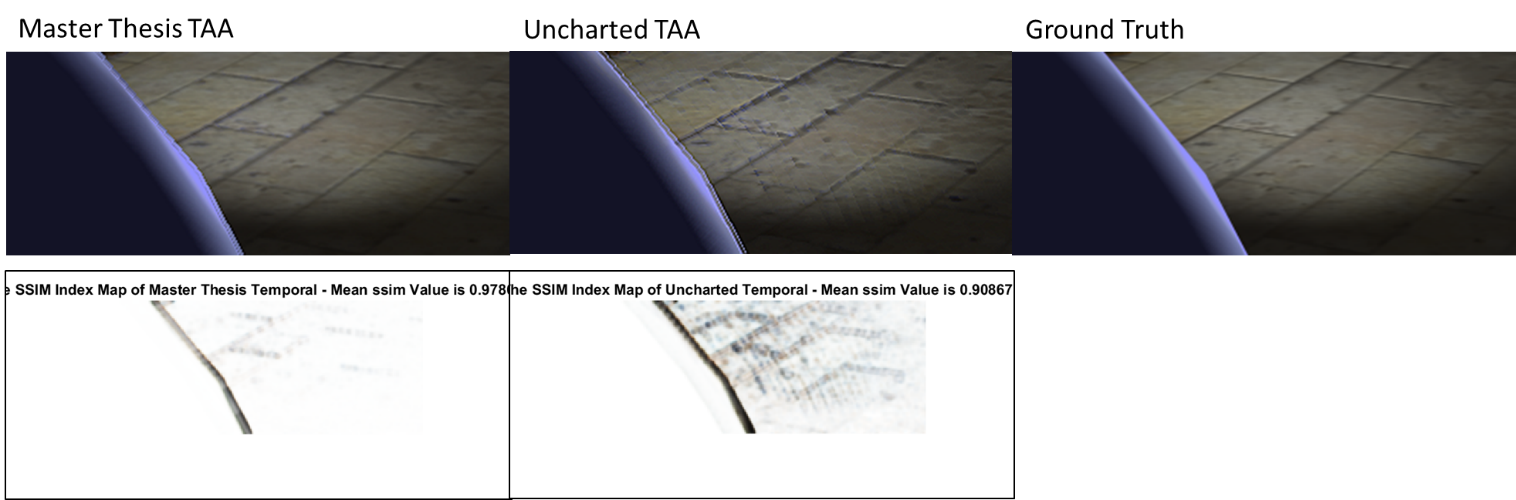
\includegraphics[scale=0.8]{images/results/sphere_ghosting.png}
	\caption{Example of Ghosting. Comparison between Master Thesis TAA, Uncharted TAA and Ground Truth on Test Number 19.}\label{fig:sphere_ghosting}
\end{figure}

\subsection{Hairball}
These tests were the hardest for all the techniques we tried. The Hairball Model contains many fibers with many details that provide a complex test for any Anti-Aliasing solution. We performed all the tests without light, to see the silhouette, and with light, to see how its reaction to the fibers affected all the Anti-Aliasing solutions. We did two sets of tests, the first one was static, to show us the behavior of blurring and aliasing correction; and the second set was rotating, to show us how ghosting behaved on the fibers. The results from the static tests were surprising, as we did not expect the Master Thesis Implementation to be the best handling the fibers because of the results in both windows tests.
\subsubsection{Static Shadow}
From Figures \ref{fig:hairball_static_shadow_render} and \ref{fig:hairball_static_shadow_truth}, we can observe that the Uncharted TAA has problems on most of the fibers, on its SSIM map this is visible as the big dark edge around Hairball; SMAA fails to correct aliasing on the smaller fibers, we observe this as the gray areas around the Hairball model on the SSIM map; and, finally, we notice that the Master TAA is the best at handling the fibers, they look smooth as in the original model, and its SSIM map has the least amount of dark areas. Also, from Table \ref{tab:hairball_static_shadow} we can confirm that the Master TAA is the best at rendering the static shadow Hairball by a relatively big margin compared to the other techniques.

% Table generated by Excel2LaTeX from sheet 'Hairball Static Shadow'
\begin{table}[!hbt]
	\small
	\centering
	\caption{Numerical results of the Hairball Static Shadow Test.}
	\begin{tabular}{|l|c|c|c|c|c|c|c|}
		\hline
		\multicolumn{8}{|c|}{\textbf{Hairball Static Shadow Test}} \\
		\hline
		\textbf{\diagbox{Tests}{AA}} & \textbf{No AA} & \textbf{FXAA}  & \textbf{SMAA}  & \textbf{\makecell{Uncharted \\ TAA}} & \textbf{\makecell{Master \\ TAA}} & \textbf{Best} & \textbf{\makecell{Master \\ TAA \\ Against \\ Best}} \\
		\hline
		MSE   & 44.367 & 21.101 & 25.379 & 88.976 & 10.293 & Master TAA & 0.000 \\
		\hline
		RMSD  & 6.661 & 4.594 & 5.038 & 9.433 & 3.208 & Master TAA & 0.000 \\
		\hline
		Peak-SNR  & 31.660 & 34.888 & 34.086 & 28.638 & 38.005 & Master TAA & 0.000 \\
		\hline
		SNR   & 18.808 & 22.036 & 21.234 & 15.786 & 25.154 & Master TAA & 0.000 \\
		\hline
		SSIM  & 0.962 & 0.978 & 0.974 & 0.934 & 0.985 & Master TAA & 0.000 \\
		\hline
	\end{tabular}%
	\label{tab:hairball_static_shadow}%
\end{table}%

\begin{figure}[H]
	\centering
	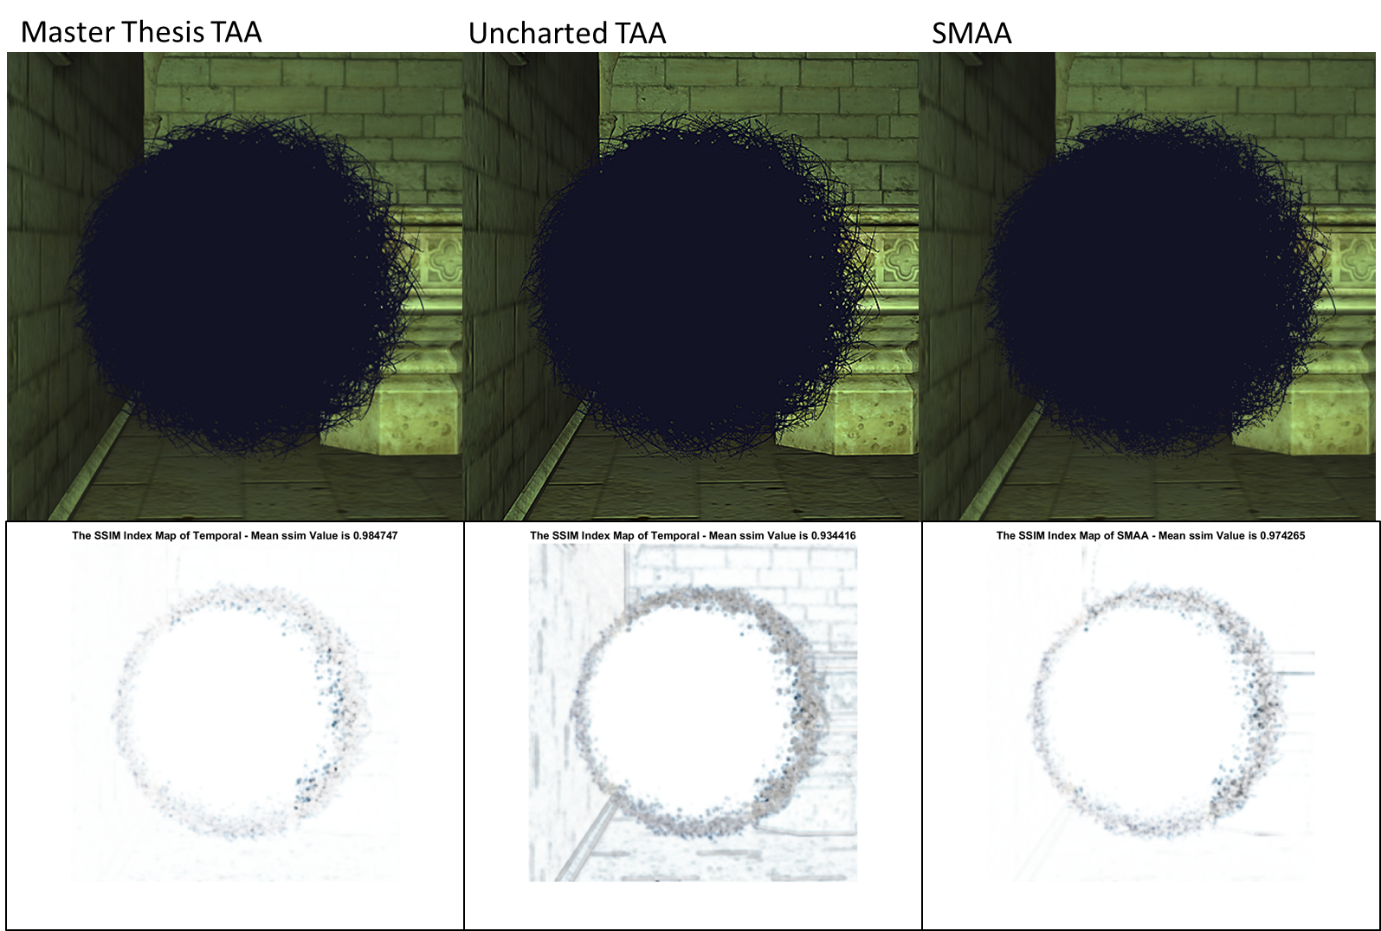
\includegraphics[scale=0.9]{images/results/hairball_static_shadow.png}
	\caption{Hairball Static Shadow comparison between Master Thesis TAA, Uncharted TAA, and SMAA.}\label{fig:hairball_static_shadow_render}
\end{figure}

\begin{figure}[H]
	\centering
	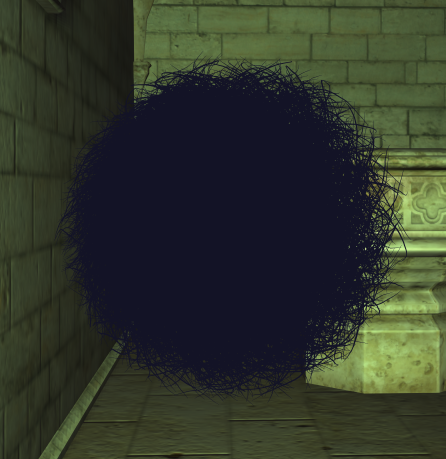
\includegraphics[scale=0.3]{images/results/hairball_sobel_ground_truth.png}
	\caption{Hairball Static Shadow ground truth.}\label{fig:hairball_static_shadow_truth}
\end{figure}


\subsubsection{Static Light}
From Figures \ref{tab:hairball_static_lighted} and \ref{fig:hairball_static_lighted_truth}, we observe that the Uncharted TAA generated wrong bright colors around all the fibers, on its SSIM this appears as the complete model is dark; SMAA fails to correct a high amount of fibers, they appear aliased on the rendered image and its SSIM map contains many dark zones; and, finally, we can observe that the Master TAA has the smoothest edges of all the rendered images, on its SSIM map and on Table \ref{tab:hairball_static_lighted} we notice that there still errors but they are smaller by a large margin compared to any other technique.

% Table generated by Excel2LaTeX from sheet 'Hairball Static Lighted'
\begin{table}[H]
	\small
	\centering
	\caption{Numerical results of the Hairball Static Light Test.}
	\begin{tabular}{|l|c|c|c|c|c|c|c|}
		\hline
		\multicolumn{8}{|c|}{\textbf{Hairball Static Light Test}} \\
		\hline
		\textbf{\diagbox{Tests}{AA}} & \textbf{No AA} & \textbf{FXAA}  & \textbf{SMAA}  & \textbf{\makecell{Uncharted \\ TAA}} & \textbf{\makecell{Master \\ TAA}} & \textbf{Best} & \textbf{\makecell{Master \\ TAA \\ Against \\ Best}} \\
		\hline
		MSE   & 1294.649 & 649.940 & 847.702 & 1444.095 & 226.567 & Master TAA & 0.000 \\
		\hline
		RMSD  & 35.981 & 25.494 & 29.115 & 38.001 & 15.052 & Master TAA & 0.000 \\
		\hline
		Peak-SNR  & 17.009 & 20.002 & 18.848 & 16.535 & 24.579 & Master TAA & 0.000 \\
		\hline
		SNR   & 8.446 & 11.439 & 10.285 & 7.971 & 16.015 & Master TAA & 0.000 \\
		\hline
		SSIM  & 0.801 & 0.865 & 0.841 & 0.785 & 0.937 & Master TAA & 0.000 \\
		\hline
	\end{tabular}%
	\label{tab:hairball_static_lighted}%
\end{table}%

\begin{figure}[H]
	\centering
	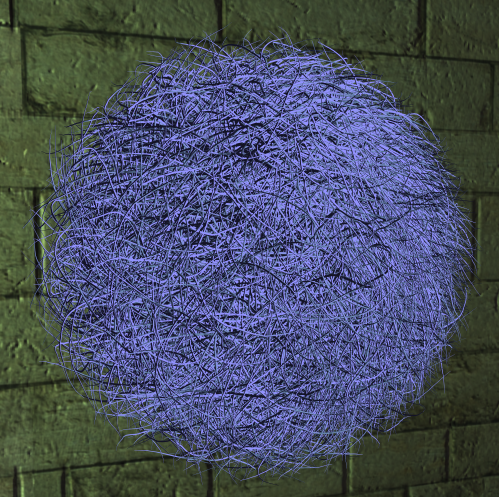
\includegraphics[scale=0.2]{images/results/hairball_light_sobel_ground_truth.png}
	\caption{Hairball Static Lighted ground truth.}\label{fig:hairball_static_lighted_truth}
\end{figure}

\begin{figure}[H]
	\centering
	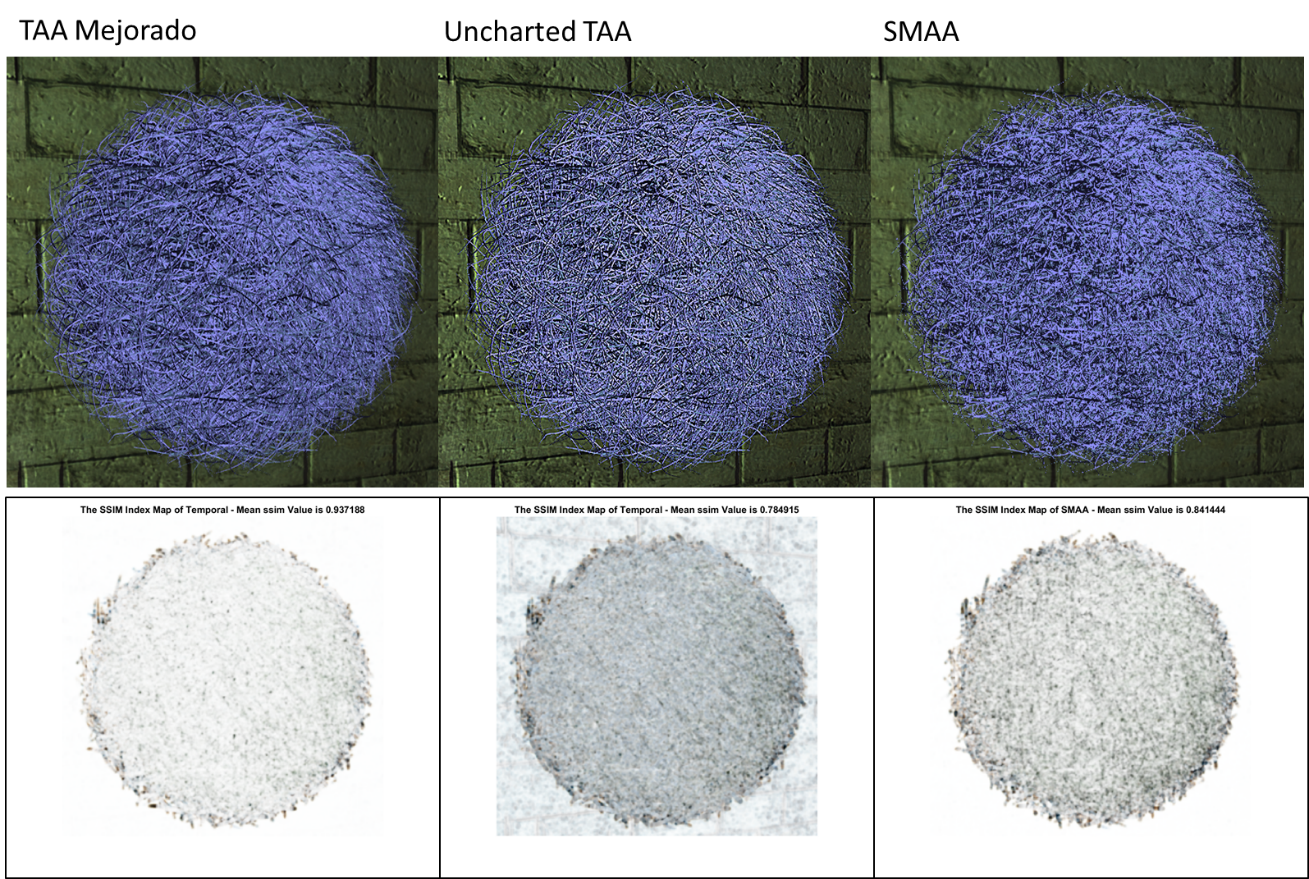
\includegraphics[scale=0.9]{images/results/hairball_static_lighted.png}
	\caption{Hairball Static Lighted comparison between Master Thesis TAA, Uncharted TAA, and SMAA.}\label{fig:hairball_static_lighted_render}
\end{figure}


\subsubsection{Ghosting Shadow}
From Figure \ref{fig:hairball_ghosting_shadow}, we can observe that both implementations generate blurriness around the fibers edges, this is visible on both SSIM maps as the dark ring around the model. On Table \ref{tab:hairball_ghosting_shadow} we observe that the Master Thesis TAA is numerically better than the Uncharted TAA. As well, the Test Index on Table \ref{tab:hairball_ghosting_shadow} marks which test the associated result belongs to; on the averages we use Not Applicable (N\\A) because those results come from the average of all the tests. 

% Table generated by Excel2LaTeX from sheet 'Hairball Ghosting Shadow'
\begin{table}[H]
	\small
	\centering
	\caption{Numerical results summary of the 100 tests performed for the Hairball Ghosting Shadow Test.}
	\begin{tabular}{|l|c|c|c|c|}
		\hline
		\multicolumn{5}{|c|}{\textbf{Hairball Ghosting Shadow Test Summary}} \\
		\hline
		\multicolumn{1}{|c|}{\textbf{\diagbox{Tests}{AA}}} & \textbf{Uncharted TAA} & \textbf{Test Index} & \textbf{Master TAA} & \textbf{Test Index} \\
		\hline
	    Best MSE & 70.261 & 17    & 32.692 & 0 \\
		\hline
		Worst MSE & 93.024 & 90    & 42.962 & 90 \\
		\hline
		Average MSE & 81.887 & N/A   & 38.534 & N/A \\
		\hline
		Best Peak-SNR & 29.664 & 17    & 32.986 & 0 \\
		\hline
		Worst Peak-SNR & 28.445 & 90    & 31.800 & 90 \\
		\hline
		Average Peak-SNR  & 29.009 & N/A   & 32.278 & N/A \\
		\hline
		Best SNR & 16.940 & 17    & 20.278 & 0 \\
		\hline
		Worst SNR & 15.846 & 90    & 19.201 & 90 \\
		\hline
		Average SNR  & 16.333 & N/A   & 19.602 & N/A \\
		\hline
		Best SSIM & 0.925 & 17    & 0.947 & 17 \\
		\hline
		Worst SSIM & 0.911 & 99    & 0.934 & 68 \\
		\hline
		Average SSIM & 0.913 & N/A   & 0.940 & N/A \\
		\hline
	\end{tabular}%
	\label{tab:hairball_ghosting_shadow}%
\end{table}%

\begin{figure}[H]
	\centering
	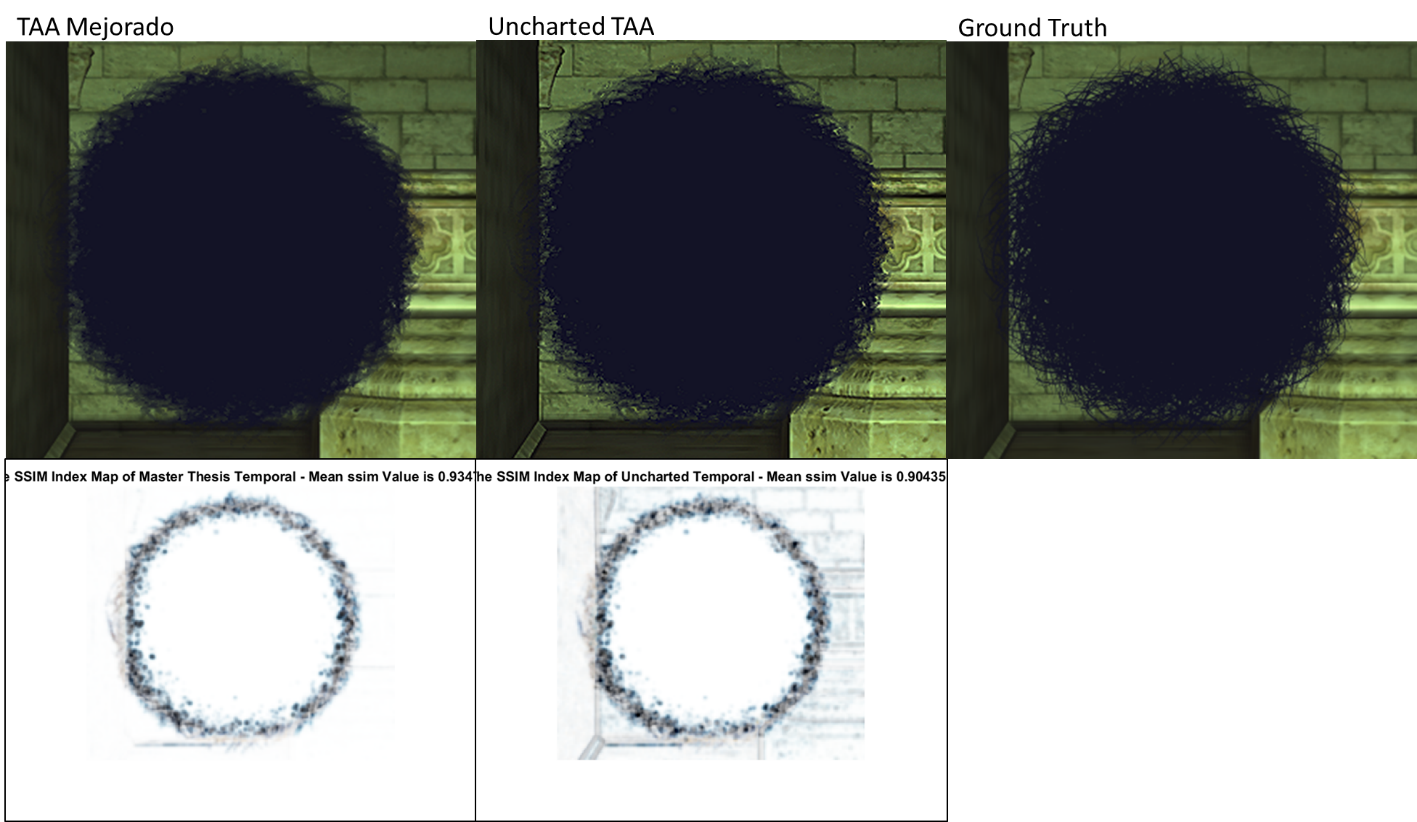
\includegraphics[scale=0.8]{images/results/hairball_ghosting_shadow.png}
	\caption{Ghosting comparison between Master Thesis TAA, Uncharted TAA and Ground Truth on Test Number 90.}\label{fig:hairball_ghosting_shadow}
\end{figure}

\subsubsection{Ghosting Light}
From Figure \ref{fig:hairball_ghosting_lighted} and Table \ref{tab:hairball_ghosting_lighted}, we observe that both techniques generate a high amount of blurring around the fibers. On both SSIM maps the blurring is visible as Hairball is seen as a big dark area. As well, the Test Index on Table \ref{tab:hairball_ghosting_lighted} marks which test the associated result belongs to; on the averages we use Not Applicable (N\\A) because those results come from the average of all the tests. 
% Table generated by Excel2LaTeX from sheet 'Hairball Ghosting Lighted'
\begin{table}[H]
	\small
	\centering
	\caption{Numerical results summary of the 100 tests performed for the Hairball Ghosting Light Test.}
	\begin{tabular}{|l|c|c|c|c|}
		\hline
		\multicolumn{5}{|c|}{\textbf{Hairball Light Shadow Test Summary}} \\
		\hline
		\multicolumn{1}{|c|}{\textbf{\diagbox{Tests}{AA}}} & \textbf{Uncharted TAA} & \textbf{Test Index} & \textbf{Master TAA} & \textbf{Test Index} \\
		\hline
		Best MSE & 714.811 & 62    & 603.190 & 1 \\
		\hline
		Worst MSE & 980.701 & 83    & 749.516 & 99 \\
		\hline
		Average MSE & 875.687 & N/A   & 671.202 & N/A \\
		\hline
		Best Peak-SNR & 19.589 & 62    & 20.326 & 1 \\
		\hline
		Worst Peak-SNR & 18.215 & 83    & 19.383 & 99 \\
		\hline
		Average Peak-SNR  & 18.737 & N/A   & 19.867 & N/A \\
		\hline
		Best SNR & 10.037 & 62    & 10.913 & 1 \\
		\hline
		Worst SNR & 8.666 & 83    & 9.902 & 99 \\
		\hline
		Average SNR  & 9.261 & N/A   & 10.390 & N/A \\
		\hline
		Best SSIM & 0.738 & 62    & 0.766 & 1 \\
		\hline
		Worst SSIM & 0.662 & 99    & 0.694 & 83 \\
		\hline
		Average SSIM & 0.691 & N/A   & 0.722 & N/A \\
		\hline
	\end{tabular}%
	\label{tab:hairball_ghosting_lighted}%
\end{table}%

\begin{figure}[H]
	\centering
	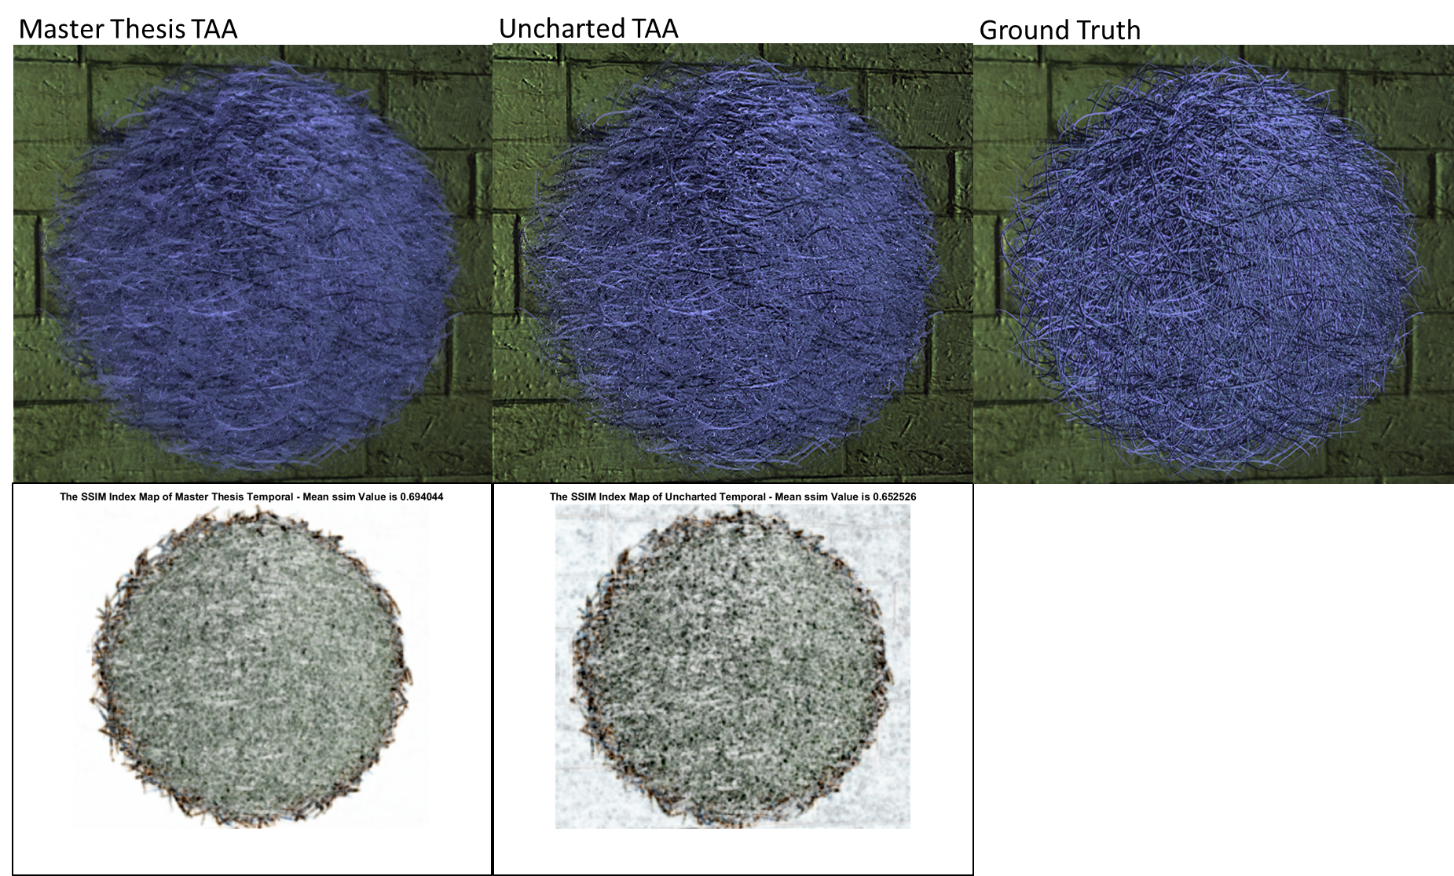
\includegraphics[scale=0.8]{images/results/hairball_ghosting_lighted.png}
	\caption{Ghosting comparison between Master Thesis TAA, Uncharted TAA and Ground Truth on Test Number 83.}\label{fig:hairball_ghosting_lighted}
\end{figure}


\subsection{Timing} \label{result_timing}
It is important to note that all the tested techniques are of Post-Processing nature, that means that they receive the output image from the Deferred Shading Architecture as input, making them not dependent on the complexity of the scene.
 
The measured time the Master Thesis TAA technique took to run was between $0.5$ and $0.6$ $ms$ on average. The Sobel pass took between $0.2$ $ms$ and $0.3$ $ms$, and the reprojection was around $0.3$ $ms$. The measured time the Uncharted TAA technique took was between $0.2$ $ms$ and $0.3$ $ms$; FXAA took between $0.1$ $ms$ and $0.2$ $ms$; and SMAA took $0.2$ $ms$ and $0.3$ $ms$.

\section{Discussion}
As we appreciate the results of the Sharpen Filter Test, see Table \ref{tab:sharpen_res}, the improvements achieved in this master thesis go beyond modifying the filter from the Uncharted implementation, because changing this filter only avoids generating those wrong bright pixels around edges. We believe that their use of that specific filter is of artistic nature. It tends to pronounce the edges at the cost of creating bright pixels around the edges that flicker, especially, when the camera moves while the foreground is illuminated but the background is on shadows or vice versa. 

From both Pipe Tests we can observe that the results from the Master Thesis TAA are close to SMAA results when drawing hard edges. We can quantify the reduction of blurring when comparing to the Uncharted TAA implementation in the numerical results from the Tables \ref{tab:pipe_regular} and \ref{tab:pipe_inclination}. When we compare the SSIM maps results (Figures \ref{fig:pipe_regular_render} and \ref{fig:pipe_inclination_render}), we observe that the thick error line around the edges in the Uncharted implementation is not present our Master Thesis implementation. But, the blurring reduction is not perfect, as we see on the tests scores, the blurring that remains around the edges lets SMAA the high score on some tests.

From the Window with Blinds and Arched Window Tests we can appreciate how the techniques react to small, almost pixel sized, features like the blinds and the doors from the Arched Window. Although the Master Thesis TAA and SMAA appear numerically (See Tables \ref{tab:window_blind} and \ref{tab:window_arch}) better than the Uncharted TAA, they are not able to reconstruct all the small details leaving pixel thin stripes that flicker when the camera moves. We believe that in this case, admitting the blurring of the Uncharted TAA benefits its final application because losing some small details is better than having many pixels flickering each time the camera moves.

The Sponza Atrium Test shows us that the Master Thesis TAA is more than capable of handling a general scene with lighting and shadows. As seen in the Table \ref{tab:sponza}, our implementation proved to be better than the other Anti-Aliasing techniques by a fair margin in almost all the tests.

We consider the Sponza Atrium Flowers Test a distinctive experiment because the flowers are a 2D flat surface with many complex transparent holes and they are rotated around the column. As we observe from the numerical results in the Table \ref{tab:sponza_flowers} and SSIM maps on Figure \ref{fig:sponza_flowers_render}, all the techniques struggle with those transparent holes but our Master Thesis TAA proves to be the best at handling them.  We see from this test that our implementation is good at handling this type of small details, compared to the Windows Tests, because they are larger than just a pixel. 

From the Hard Edges Test we continue to observe that the Master Thesis technique handles better the blur compared to the Uncharted TAA (See Table \ref{tab:hard_test}), especially on the letters, the pipe, and the square; and that the Master Thesis technique still has a hard time handling the super fine details from the windows, at this distance we still believe the blurring of the Uncharted TAA helps to hide the unwanted pixel stripes that flicker (See Figure \ref{fig:hard_test_render}).

In the Sphere Ghosting Test we see a clear example of the improvements accomplished in this Thesis. Figure \ref{fig:sphere_ghosting} shows one example of the ghosting that is created by the Uncharted TAA implementation, we can clearly perceive the stripes that are left by the sphere while it moves, whereas on our Master Thesis TAA implementation they are barely visible.

Finally, we have the four Hairball Tests, the most complex tests performed. The Hairball model has many gaps and small details that react to lighting and shadows. We anticipated a high amount of errors due to them because all Anti-Aliasing techniques have difficulties reconstructing this high density of fine details. 

On the Shadow and Light Static Test (See Tables \ref{tab:hairball_static_shadow} and \ref{tab:hairball_static_lighted}) we can observe that the Master Thesis Implementation is the best at handling the hair fibers. It is able to reconstruct smoother edges than the Uncharted TAA and reconstructs more details than SMAA technique. Especially on the light version (See Figure \ref{fig:hairball_static_lighted_render}), we can appreciate how smooth the result is; it looks almost like the ground truth. This test far exceeded the expectation of our improvements, the visual and numerical (See Table \ref{tab:hairball_static_lighted}) results shows a big increase in quality compared to the other Anti-Aliasing solutions.

On the Shadow and Light Ghosting Test we observe that both techniques results are blurred excessively (See Figures \ref{fig:hairball_ghosting_shadow} and \ref{fig:hairball_ghosting_lighted}), especially the Master Thesis TAA implementation on the light version. We believe this to be caused by the History Buffer and the Sobel Temporal Pass, for the Master Thesis TAA, not being able to stabilize as fast as the colors change when the fibers move thanks to the color rejection being slower than needed. The numerical values from Tables \ref{tab:hairball_ghosting_shadow} and \ref{tab:hairball_ghosting_lighted} confirm the effects of blurring thanks to the MSE being higher than normal.


From our timing results (See \ref{result_timing}), we can see that our improvements fit the time requirements to run on real-time applications as it is below the $1$ $ms$ common limit.


\chapter{Conclusions and Recommendations}
As we have shown numerically and visually with the tests performed, the Master Thesis implementation accomplished its objective of reducing the effects of blurring and ghosting of the Temporal Anti-Aliasing technique with the use of edge detection of both color and depth, and triangle indexing. Our results show that this technique can provide the same or better quality than other standard Anti-Aliasing solutions. 

As possible improvements, we are confident that our implementation could be optimized to run faster than our current timing. Our current implementation was made with flexibility in mind to help us test different approaches. This could be simplified to reduce the number of passes required. 

As for recommendations for further research, we suggest improving the technique's behavior under high detail density moving objects, like on the Hairball Tests. Another improvement subject is the stability for pixel size details that cause flickering, like on the Windows Tests. Furthermore, a Specular Lighting Anti-Aliasing solution compatible with Temporal Anti-Aliasing is still required to provide a full range solution to Aliasing in real-time applications. Also, we suggest searching for more specific Image Metrics for Computer Graphics, especially, finding tuning values for SSIM to provide more numerical resolution when comparing different rendered images.


\bibliography{MyMSc}

\appendix
\chapter{GitHub Repository}
The main link to the repository is https://github.com/maniatic0/Christian-TRAA . From there, the next links can be accessed for the printed version of this report.
\begin{itemize}
	\item Full Repository: https://github.com/maniatic0/Christian-TRAA.
	\item Complete Computer Specification: \\ https://github.com/maniatic0/Christian-TRAA/tree/master/PC\%20Specification.
	\item All Tests: \\ https://github.com/maniatic0/Christian-TRAA/tree/master/Important\%20Tests.
	\item Accumulation Buffer Tests: \\ https://github.com/maniatic0/Christian-TRAA/tree/master/Important\%20Tests/Accumulation\%20Buffer\%20Tests.
	\item Most of the Master Thesis Tests: \\ https://github.com/maniatic0/Christian-TRAA/tree/master/Important\%20Tests/Master\%20Thesis\%20Tests.
	\item Sharpening Tests: \\ https://github.com/maniatic0/Christian-TRAA/tree/master/Important\%20Tests/Sharpening\%20Tests.
	\item Ghosting Tests: \\ https://github.com/maniatic0/Christian-TRAA/tree/master/Important\%20Tests/Ghosting.
	\item HairBall Tests: \\ https://github.com/maniatic0/Christian-TRAA/tree/master/Important\%20Tests/HairBall.
	\item Code: \\ https://github.com/maniatic0/Christian-TRAA/tree/master/CG\_Labs.
	\item \LaTeX Report: \\ https://github.com/maniatic0/Christian-TRAA/tree/master/LaTeX/Master\_Thesis.
\end{itemize}
\chapter{Camera Jittering Explanation} \label{appendix:jitter}
The $Halton Sequence (2, 3)$ generates points in the $[0,1]\times [0,1]$ space. First, we need to transform it to the $[-1,1]\times [-1,1]$ space because we consider the pixel to be at the center, i.e. in OpenGL the first pixel is at $(0.5, 0.5)$, so we apply the transformation $T_1(x, y) = 2 * (x, y) – (1, 1)$.

Now, we only want to jitter inside the pixel because we should only be sampling inside of it. We want to control this but for explanation purposes, we can assume that we only want it inside the pixel. So, we apply the transformation $T_2(x, y) = \frac{(x, y)}{2}$.

From now on, we need to change how we interpret the process we are performing; we are calculating the distance we are going to move the pixel center, so we need to see it as a vector rather than a point. We need to transform the vector to a vector normalized by the screen size. Consequently, we apply the transformation $T_3(x, y) = (x, y) / (w, h)$ with $(w, h)$ being the Width and Height of the screen and “$/$” operator as component-wise division.

Now we need to transform our vector normalized by the screen size $[0, 1]$ to the Normalized Device Coordinates which go in the range $[-1, 1]\times [-1, 1]$. This is done by using $T_4(x, y) = 2 * (x, y)$ (to transform points we would use $2*(x, y) – (1, 1)$).
At the end, our transformation would look like this $T(x, y) = T_4(T_3(T_2(T_1(x, y)))) = (2 * (x, y) – (1, 1)) / (w, h)$ with $(x, y)$ being a Halton Sequence point.

We now need to modify our Projection Matrix, which takes points from the View Space into the Clip Space. The resulting matrix is taken from the Ke Xu presentation page 14 ~\cite{XU2016}. Let $(h_x,h_y)$ be jitter we have previously calculated.

\begin{equation}
\begin{split}
JitteredProjection = & \begin{bmatrix*} 
a & 0 & h_x & 0 \\ 
0 & b & h_y & 0 \\
0 & 0 & c & d   \\
0 & 0 & -1 & 0   \end{bmatrix*} = JitterMatrix\times Projection \\
= & \begin{bmatrix*} 
1 & 0 & 0 & -h_x \\ 
0 & 1 & 0 & -h_y \\
0 & 0 & 1 & 0   \\
0 & 0 & 0 & 1   \end{bmatrix*} \times \begin{bmatrix*} 
a & 0 & 0 & 0 \\ 
0 & b & 0 & 0 \\
0 & 0 & c & d   \\
0 & 0 & -1 & 0   \end{bmatrix*}
\end{split}
\end{equation}

Let’s see its effect to a point in View Space, let $p_{view}=(x,y,z,1)$.

\begin{equation}
	JitteredProjection\times p_{view} = \begin{bmatrix*}
	a*x+h_x*z \\
	b*y+h_y*z \\
	c*z+d \\
	-z
	\end{bmatrix*}
\end{equation}

We proceed to do the Perspective Divide to transform the point to NDC Coordinates, this is accomplished by dividing the vector by the w component.

\begin{equation}
\begin{bmatrix*}
-a*\frac{x}{z}-h_x \\
-b*\frac{y}{z}-h_y \\
-c+\frac{d}{z}d \\
1
\end{bmatrix*} = p_{NDC} + \begin{bmatrix*}
-h_x \\
-h_y \\
0 \\
0
\end{bmatrix*}
\end{equation}

Accordingly, we only need to be sure we can apply the Jitter Matrix alone to use it inside Pixel Shaders with points in NDC space. 

\begin{equation}
	JitterMatrix\times p_{NDC} = \begin{bmatrix*}
	x_{NDC}-h_x \\
	y_{NDC}-h_y \\
	z_{NDC} \\
	1
	\end{bmatrix*} = p_{NDC} + \begin{bmatrix*}
	-h_x \\
	-h_y \\
	0 \\
	0
	\end{bmatrix*}
\end{equation}



\end{document}